\chapter{The Near Detector Liquid Argon TPC}
\label{ch:lartpc}

\fixme{Note: the R/O link for the CDR chapter on ND-LAr is https://www.overleaf.com/read/djjrpnnxzbfp}

%%%%%%%%%%%%%%%%%%%%%%%%%%%%%%%%%%%%%%%
\section{Overview of ND-LAr}\label{sec:lartpc-ovvw}
%%%%%%%%%%%%%%%%%%%%%%%%%%%%%%%%%%%%%%%
%{\it Jonathan, with help from Dan D., 5 pages}

One of the key aspects of the DUNE near detector is its ability to reduce cross section and detector systematic uncertainties in the oscillation analysis. One of the most direct ways to accomplish this is to have the target material of the near detector match that of the far detector. In the case of DUNE, this means ensuring a liquid argon (LAr) detector as part of the DUNE near detector complex. 

A problem is given the relatively slow readout of conventional monolithic liquid argon time projection chambers (LArTPC's), the extremely high neutrino flux expected in the near detector, and the large number of events; common wire-based readouts would be stretched beyond their ability to reconstruct events with high fidelity. 

A new generation of LArTPC's based on a more flexible modular design and powerful new native 3D pixel readout allows for a LArTPC to overcome the challenges of operating in the DUNE near detector environment. This design of LArTPC, based on the ArgonCube technology, utilizes thin materials to minimize the dead material introduced through modularization and new dielectric light detection techniques to leverage the optical segmentation and increase the light yield in each module. When these two techniques are coupled with pixelized charge readout, which provides unambiguous
3D imaging of particle interactions, a powerful new LArTPC detector capable of providing the necessary measurements needed by the DUNE oscillation physics measurements can be realized.

The LAr component (ND-LAr) of the DUNE ND is made up of a configuration of ArgonCube LArTPCs large enough to provide the required hadronic shower containment and statistics. NDLAr is the most upstream of the three subdetectors in the DUNE ND complex.

The subsequent sections will lay out the details of the ND-LAr system. Section \ref{sec:lartpc-ovvw-intro} will provide an overview of the detector principle and an overview of the scope of the ND-LAr consortium. Section \ref{sec:lartpc-ovvw-op}.....



%%%%%%%%%%%%%%%%%%%%%%%%%%%%%%%%%%%%%%%%%%
\subsection{Introduction and Scope}\label{sec:lartpc-ovvw-intro}
%%%%%%%%%%%%%%%%%%%%%%%%%%%%%%%%%%%%%%%%%%


As outlined in the section \ref{intro:science:role}, the overall role of the near detector complex is to provide measurements  ``... of sufficient precision to ensure that when extrapolated to \dword{fd} to predict the \dword{fd} event spectra, the associated systematic error must not dominate the measurement precision.'' The ND-LAr detector accomplishes this both as a stand-alone detector and as part of the overall ND complex in a number of ways.

As a standalone detector the LAr-ND detector will provide:
\begin{itemize}
    \item High statistics sample of beam neutrino interactions on argon which enable the a precise predication of the far detectors expected signal (excluding non-contained events) 
    \item High statistics sample of $\nu-Ar$ interactions for use in validating the far detectors neutrino-nucleus interaction models, detector models, reconstruction techniques, and systematic studies.
    \item Direct flux constraints through two unique samples enabled by the high interaction rate in the liquid argon, namely $\nu-e$ elastic scattering and leveraging the low-$\nu$-CC $\nu_\mu$ technique
\end{itemize}

As part of the overall ND complex, the ND-LAr detector also works in tandem with the other systems to:

\begin{itemize}
    \item Fully reconstruct $\nu-Ar$ interactions by matching non-contained events with the downstream muon spectrometer (TMS)
    \item Move off axis as part of the PRISM concept to provide samples of $\nu-Ar$ interactions at varying neutrino energy
    \item Monitor the flux (when on axis) and provide independent validation of the relevant beam parameters %%% this last point might be BS 
\end{itemize}

The full LAr-ND system is described in the subsequent sections and is shown in overview in Figure \ref{}. In overview, the system consists of xx optically separated LArTPC modules to allow for independent identification of $\nu-Ar$ interactions using optical timing and enabling neutron tagging using the light system in the high pile-up environment. Each TPC consists of a high voltage cathode, a low profile field cage to minimize the amount of inactive material between modules, a light collection system, and a pixel based charge readout. 

The modules are hosted in a common purified bath of liquid argon which is held within a custom designed membrane cryostat. The cryostat and adjacent mezzanine cyogenics is placed on a mobile PRISM platform to allow for the entire detector to be shifted off-axis relative to the neutrino beam. The full system is serviced by flexible energy chains enabling the motion of the full LAr-ND.
{\it Insert figure of ND LArTPC detector system, with labels.}

The LAr-ND detector effort has been organized as a DUNE consortium with the consoritum taking reponsibility for the deliever of the LArTPC module and their supporting warm electronics, readout electronics, high voltage delivery system, and associated power supplies. Each of these subcomponents is described in more detail the later subsections. 

An individual TPC module consists internally of a low density profile cathode and field cage, a pixelated charge readout plane and associated low power electronics, a high coverage light readout system, the necessary module support structures including both internal cryogenics and monitoring as well as mechanical interfaces with the cryostat, and dedicated calibration systems. Externally, the TPC module has a high voltage deliever system and associated warm electronics and power supplies which enable the function of the various readout and calibration systems. 

In addition to the hardware, the LAr-ND consortium will also take responsibility for the management of integration and testing of the LArTPC modules and components. This includes the dedicated QC testing of individual and integrated systems as well as assembly and operation of the full module (e.g. at the Module Integration Facility) prior to delivery to the near site.

Once delivered to the near site, the consortium will support the installation work in cooperation with the project's near site integration team to realize the successful deployment of the modules into the near detector.

Insert interfaces here.....Cryostat, Cryogenics, DAQ/Controls, Near Site Integration


{\it Insert Figure of ND LArTPC single module, with labels.}


%%%%%%%%%%%%%%%%%%%%%%%%%%%%%%%%%%%%%%%%%
\subsection{Principle of Operation}\label{sec:lartpc-ovvw-op}
%%%%%%%%%%%%%%%%%%%%%%%%%%%%%%%%%%%%%%%%%

While many innovative technologies can be found in the design of the LAr-ND. The operating principles of the detector itself are largely the same of any liquid noble time projection chamber. As charged particles traverse the bulk material they produce ionization electrons and scintillation photons. An external electric field allows the ionization electrons to drift towards the anode of the detector and be collected on charge sensitive readout. The combined measurement of the scintillation light, providing the $t_0$, and the arrival time of the ionization charge allows for the 3D reconstruction of the original charged particle topology within TPC. Thus the TPC provides a fully active tracking detector with calormetric reconstruction capabilities without instrumenting the bulk volume of the detector.

The LBNF neutrino beam directed at the LAr-ND generates intense pulse of few-GeV-energy neutrinos each spill. These neutrinos are mostly muon flavor (with negligible oscillation at NS). The interactions of these neutrinos generates energetic lepton (mostly GeV-scale muons), and recoiling hadronic component from nucleus. The muon generally exits LArTPC as the ND-LAr alone begins to lose acceptance for muons above $\sim0.7$ GeV/c due to lack of containment. Because the muon momentum and charge are critical components of the neutrino energy determination, a magnetic spectrometer is needed downstream of ND-LAr to measure both quantities. The dimensions of the LAr-ND module have been chosen to optimize the containment of the complex hadronic showers which can result from the neutrino interaction within the active volume of the LArTPC. The corresponding scintillation light which is detected in tandem with the ionization charge produced by lepton/hadron interactions provides complementary measurement of signal position and energy, albeit at much lower granularity, but with substantially more accurate timing ($\sim$20~ns)

This detector has the same target nucleus and uses the same fundamental detection principles as the FD. The differences between the two are needed because of the expected intensity of the beam at the ND. The use of the same target nucleus and a similar technology reduces sensitivity to nuclear effects and detector-driven systematic uncertainties in the extraction of the oscillation signal at the FD. ND-LAr is large enough to provide high statistics ($1 \times 10^8 \nu_\mu$-CC events/year on axis) and a sufficient volume to provide containment of the hadronic system. The tracking and energy resolution, combined with the fiducial mass of ND-LAr, will allow for the measurement of the flux in the beam using several techniques, including the rare process of $\nu - e$ scattering. 

{\it Insert image of typical numu CC interaction in ND LArTPC, maybe also showing muon into TMS?}


One key aspect of the LAr-ND operation is its ability to cope with the large number of neutrino interactions present in each spill. As is discussed in Section \ref{sec:ndlar-pileup}, the LBNF neutrino beam consists of a 10 $\mu$s wide spill, with $\mathcal{O}$(ns) bunch structure, delivered at a $\sim 1$~Hz rate. This means that there will be $\mathcal{O}$(50) $\nu$/spill. Given the relatively low expected cosmic ray rate during the beam (estimated to be $\sim$0.3/spill at 60-m depth), this beam related pile-up is the primary challenge confronting the reconstruction of the ND-LAr events. The 3D pixel charge will readout continuously the slow drifting electrons (with charge from the cathode taking $\sim 300 \mu$s to arrive across the 50~cm distance) with an arrival time accuracy of 200~ns and a corresponding charge amplitude within a $\sim 2\mu$s wide bin. This coupled with the beam spill width gives a position accuracy of $\sim$16~mm. While this is already quite a good spatial positioning, the ND light system will provide an even more accurate time-tag of the charge as well as the ability to tag sub-clusters and spatially disassociated charge depositions resulting from neutral particles (such as neutrons) coming from the neutrino interaction. Thus the ND light system has different role than FD; as it must time-tag charge signal sub-clusters to enable accurate association of all charge to proper neutrino event (accuracy), and reject pileup of charge from other neutrino signals (purity).

{\it Insert image of single LBNF beam spill in ND LArTPC from Brooke's study.}
 
%%%%%%%%%%%%%%%%%%%%%%%%%%%%%%%%%%%%%%%%%%%%%%%
\subsection{Design Parameters}
\label{sec:lartpc-ovvw-param}
%%%%%%%%%%%%%%%%%%%%%%%%%%%%%%%%%%%%%%%%%%%%%%%
ND LArTPC design parameters driven by two major themes:
\begin{itemize}
    \item Provide signal fidelity at least as good as FD (e.g. motivates LArTPC similar to FD design).  Drives many detector attributes:
    \begin{itemize}
        \item size: hadronic containment
        \item detector spatial/temporal/energy resolutions: as good or better than FD
        \item detector systematics: field strength, uniformity, purity, etc.
    \end{itemize}
    \item Cope with ND pileup (i.e. motivates detector different than FD design):
    \begin{itemize}
        \item 3D pixelated readout: no spatial ambiguities in high pileup environment
        \item optical segmentation: accurately associate disconnected charge clusters to correct primary event
        \item high-coverage light detection: provide light-based time/position/amplitude signal resolutions to enable accurate charge signal clustering. [Note: T0 performance is not as important as for FD light system, given narrow beam spill time (10 us).  T0 still useful for non-beam signal studies (e.g. cosmic rays, 39Ar, BSM physics?).]
    \end{itemize}
\end{itemize}

%The key driving design requirements and performance requirements are summarized in Table~\ref{tab:table-ndlar-params}. 
The key driving design requirements and performance requirements are summarized in Figures~\ref{fig:lartpcreq1}~ - \ref{fig:lartpcreq4}. 
%\begin{dunetable}
%[Key System Requirements]
%{ccccccc}
%{tab:table-ndlar-params}
%{Key System Requirement}
%Rows & Counts \\ \toprowrule
%Row 1 & First \\ \colhline
%Row 2 & Second \\ \colhline
%Row 3 & Third \\ % no \colhline on final row
%\end{dunetable}


\begin{figure}
\centering 
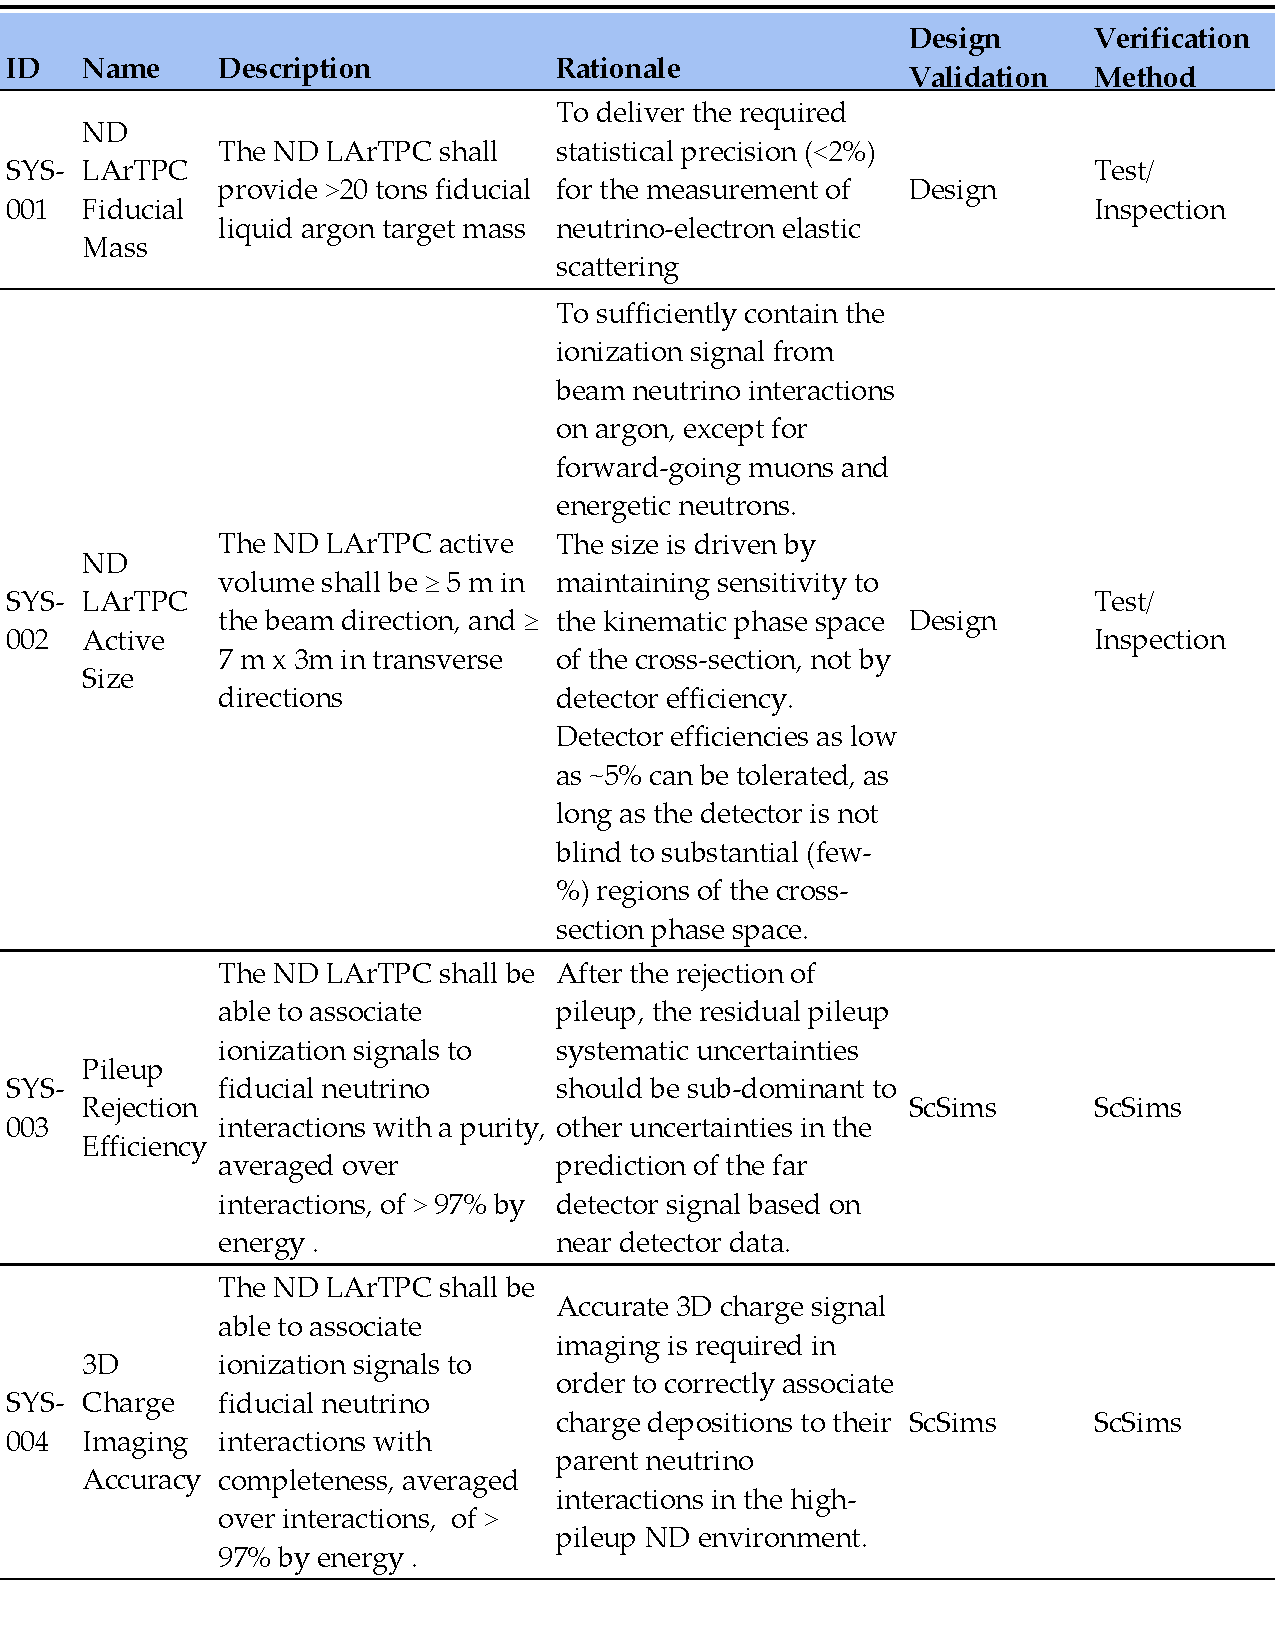
\includegraphics[width=1\linewidth]{graphics/lartpc/0Req/NDreqs1.pdf}
\caption{\label{fig:lartpcreq1} ND LArTPC Key System Requirements (1)}
\end{figure}
\begin{figure}
\centering 
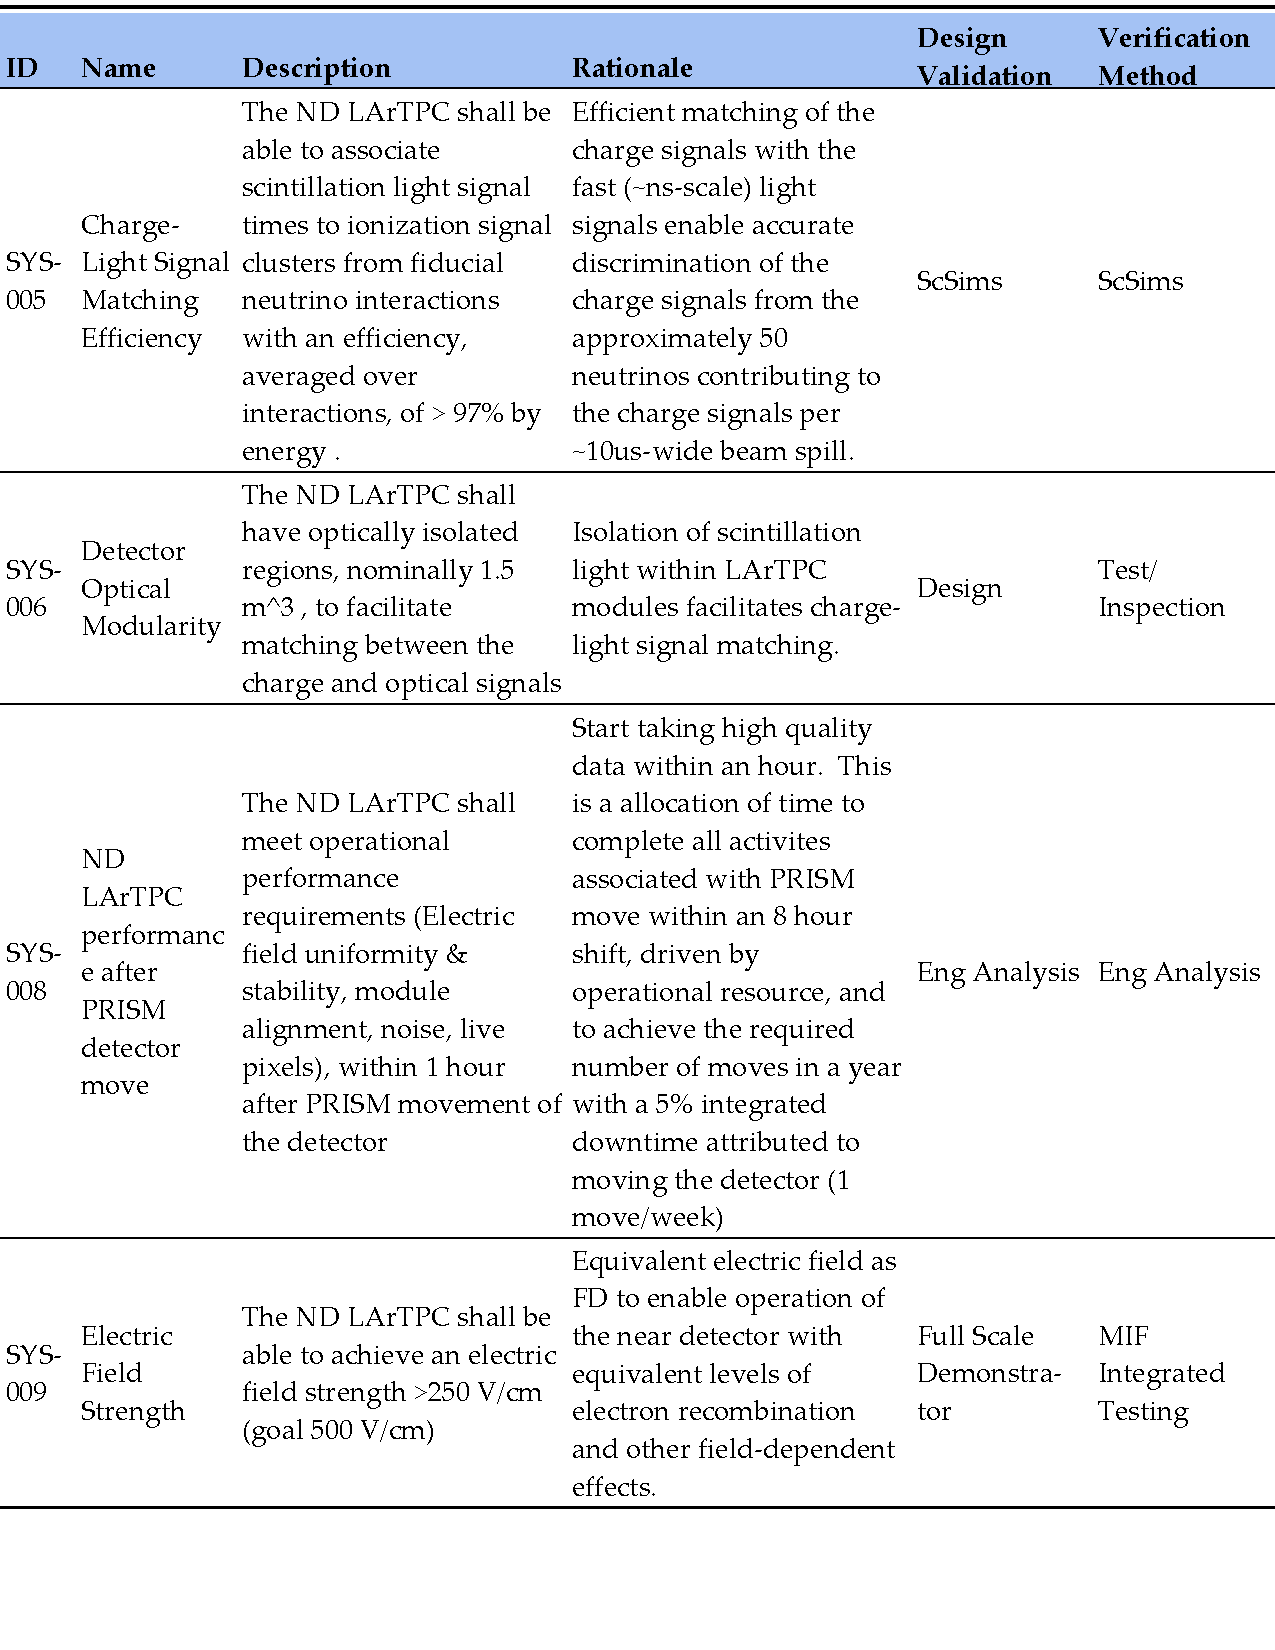
\includegraphics[width=1\linewidth]{graphics/lartpc/0Req/NDreqs2.pdf}
\caption{\label{fig:lartpcreq2} ND LArTPC Key System Requirements (2)}
\end{figure}
\begin{figure}
\centering 
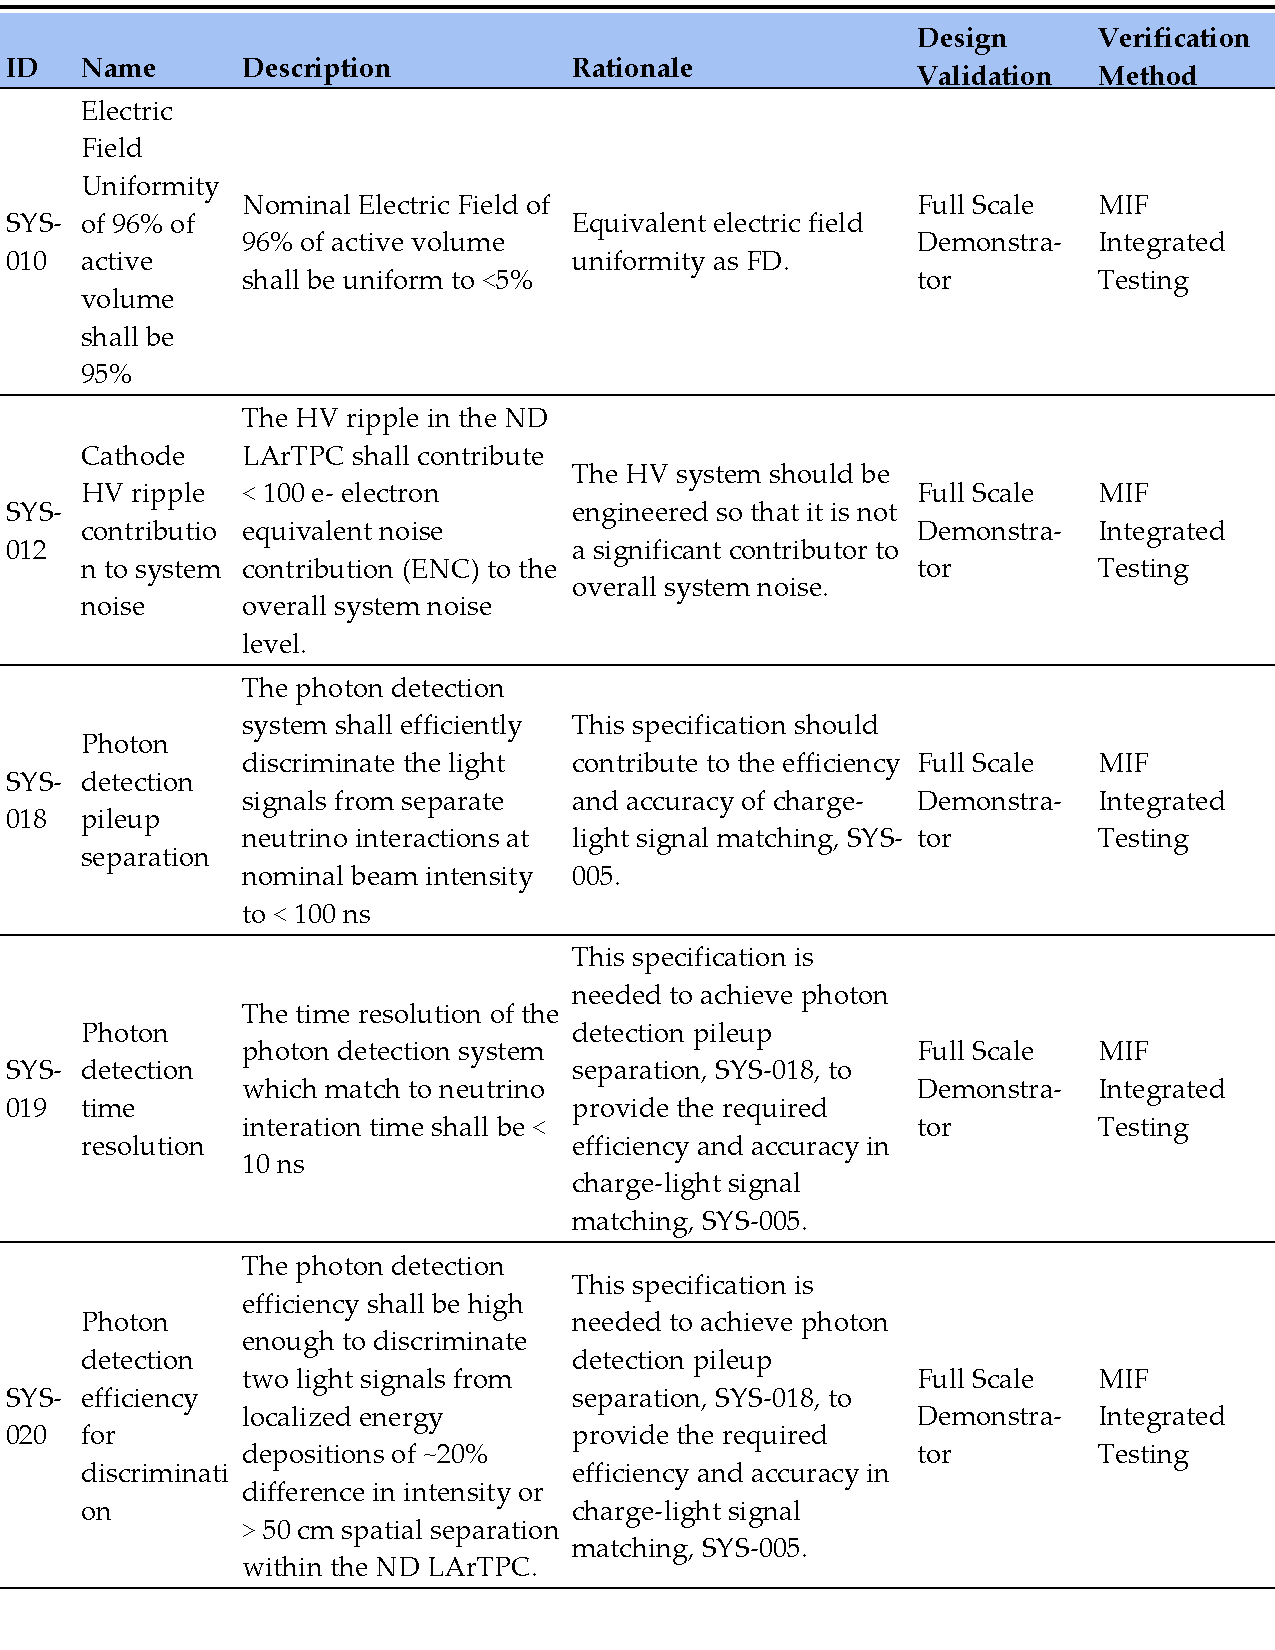
\includegraphics[width=1\linewidth]{graphics/lartpc/0Req/NDreqs3.pdf}
\caption{\label{fig:lartpcreq3} ND LArTPC Key System Requirements (3)}
\end{figure}
\begin{figure}
\centering 
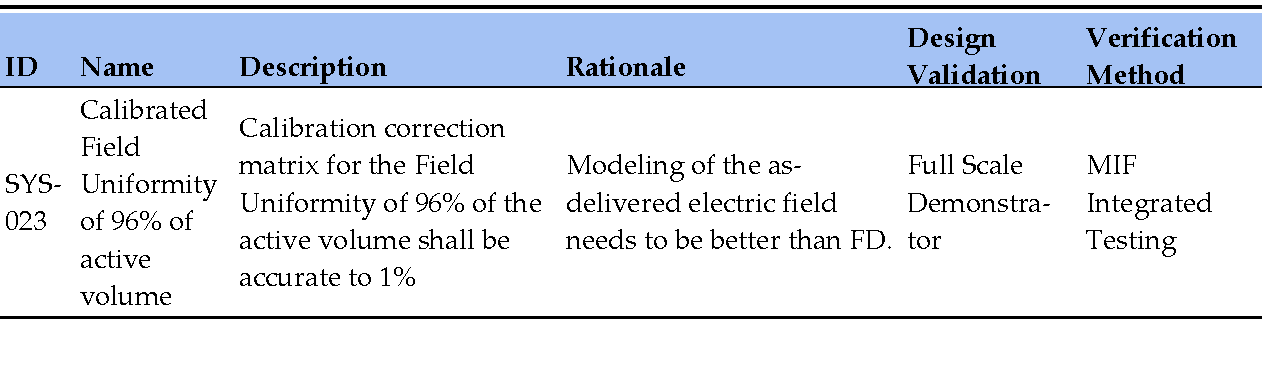
\includegraphics[width=1\linewidth]{graphics/lartpc/0Req/NDreqs4.pdf}
\caption{\label{fig:lartpcreq4} ND LArTPC Key System Requirements (4)}
\end{figure}

%%%%%%%%%%%%%%%
\subsection{Performance}
\label{sec:lartpc-ovvw-perf}
%{\it Andy M., Chris M., 4-6 pages}

The performance characteristics of ND-LAr are driven by physics requirements for the samples entering the long-baseline oscillation analysis. For example, well-matched reconstruction performance and kinematic acceptance are important for joint analysis and mitigating systematic uncertainties. Additionally, with the dense target and intense beam, the ND-LAr must be capable of uniquely reconstructing the tens of neutrino interactions expected per spill, maintaining high efficiency and minimal bias in this high-pileup environment. This section describes the high-level detector performance parameters relevant to the joint LBL analysis, including inputs based on a fully simulated and reconstructed event samples with a realistic detector geometry and beam conditions.

\subsubsection{ND-LAr key measurements}

Measurements made in ND-LAr feed directly into long-baseline neutrino oscillation analyses. The role of these measurements is to constrain systematic uncertainties on the neutrino flux and neutrino-argon interaction cross sections. The key measurements fall into three broad categories:

\begin{itemize}
    \item Charged-current $\nu_{\mu}$ as a function of off-axis angle
    \item Direct flux constraints: $\nu-e$ elastic scattering and low-$\nu$ CC $\nu_{\mu}$
    \item Exclusive, multidimensional $\nu$-Ar measurements
\end{itemize}

ND-LAr must be capable of identifying and selecting events in the various categories, and measuring key kinematic quantities precisely and without bias. The primary function of CC $\nu_{\mu}$ inclusive scattering measurements is to use linear combinations of samples at different off-axis angles to build oscillated \dword{fd} spectra. The reconstructed neutrino energy must be measured by combining a calorimetric measurement of the hadronic system with a measurement of the outgoing muon. Both of these must match or exceed the precision of the \dword{fd}. The acceptance will be different in ND-LAr and \dword{fd}, and must be corrected. This can be done directly with data except in kinematic regions where the ND-LAr acceptance is less than 10\%.

Direct flux constraints are critical because they break a degeneracy between flux and cross section uncertainties. Neutrino-electron elastic scattering is a pure electroweak process with known cross section at tree level. The signal is a single, forward electron with no other final-state particles. Selecting $\nu+e$ events requires precise reconstruction of $E_{e}\theta_{e}^{2}$, which places requirements on the electromagnetic shower reconstruction, and especially the energy and angular resolution of electromagnetic showers. Low-$\nu$ CC $\nu_{\mu}$ scattering has a cross section that is independent of neutrino energy in the limit where the hadronic energy approaches zero. This enables a direct measurement of the flux shape, but requires precise calibration of the muon energy scale, and also the ability to identify events with very small hadronic energy. Tagging final-state fast neutrons, even if their energy cannot be precisely measured, is valuable.

Finally, ND-LAr exclusive measurements provide constraints on neutrino-argon interactions. The high rate of ND-LAr enables high-statistics, highly multi-dimensional measurements, where the allowed granularity will likely be limited by detector resolution. Separating events into various exclusive samples greatly enhances the constraining power. Interesting CC samples include $0\pi$, $1\pi^{+}$, $1\pi^{0}$, and multi-pion. Measurements should be made as a function of both lepton kinematics ($E_{\mu}$ and $\theta_{\mu}$ or transverse momentum $p_{T}$), and details of the hadronic system ($E_{\pi}$ and $\theta_{\pi}$, or $Q^{2}$). These measurements require muon reconstruction, particle identification 
(especially charged and neutral pion identification), and hadronic energy reconstruction.

\paragraph{Event rates} \textcolor{red}{(CDR)}

In the oscillation region of $\SI{0.5} < E_\nu < \SI{4}{\giga\electronvolt}$, the expected event rate in the \SI{50}{\tonne} fiducial volume of \dword{ndlar} is 59 million \numu \dword{cc} interactions per year in \dword{fhc} mode and 20 million \anumu \dword{cc} interactions per year in \dword{rhc} mode. Of those, over 24 million (10 million) are expected to have a well-reconstructed muon of the appropriate sign, and a well-contained hadronic system in \dword{fhc} (\dword{rhc}). In addition, 450,000 $\nue+\anue$ \dword{cc} interactions are expected per year in \dword{fhc}, and 200,000 in \dword{rhc}. The expected event rate per one year of exposure on axis is shown in Figure~\ref{fig:argoncube_eventrate} as a function of true neutrino energy.

\begin{dunefigure}[Neutrino interaction rates in the \SI{50}{\tonne} \dword{arcube} fiducial volume]{fig:argoncube_eventrate}
{The rate of \dword{cc} interactions in the fiducial volume of \dword{ndlar} as a function of true neutrino energy, expressed per year of exposure assuming \SI{1.2}{\mega\watt} beam intensity in \dword{fhc} (left) and \dword{rhc} (right) beam polarity.}
	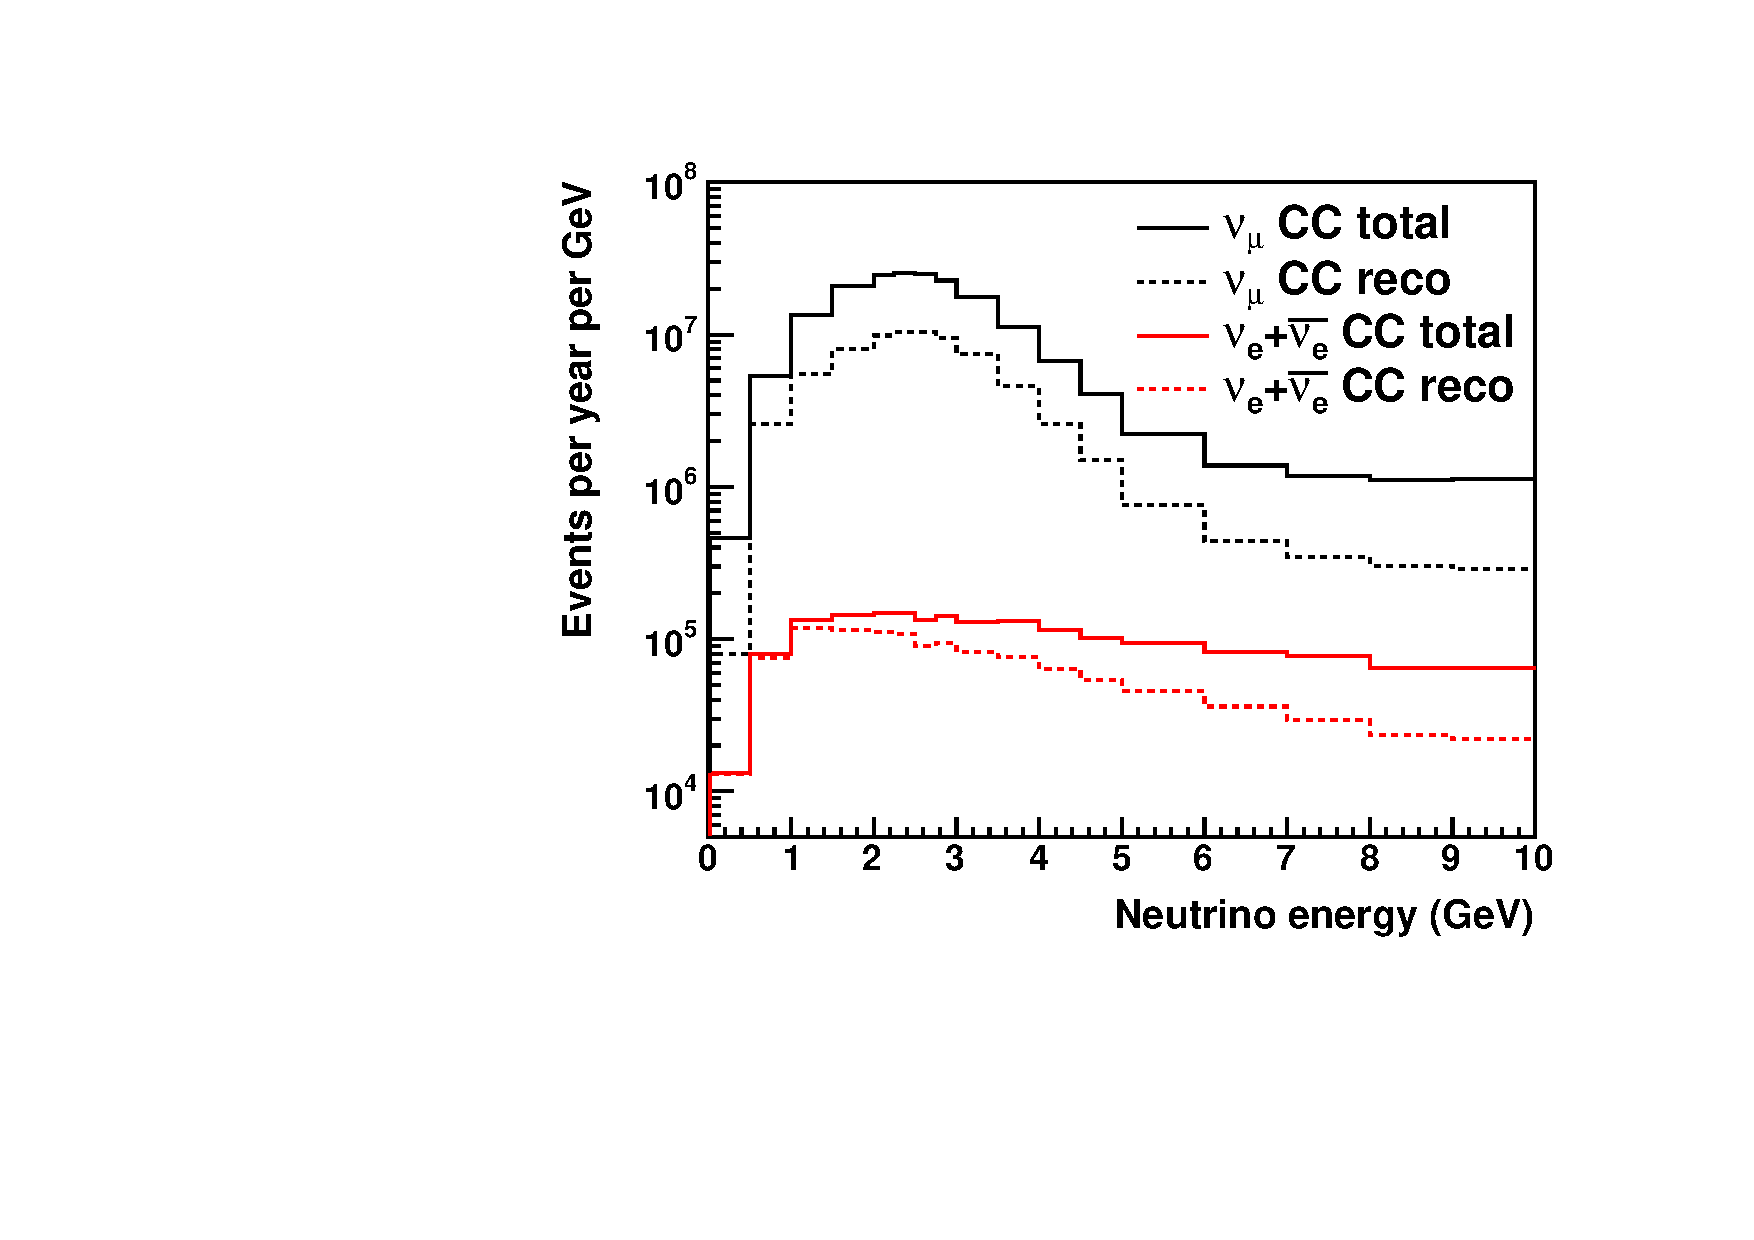
\includegraphics[width=0.48\textwidth]{graphics/lartpc/event_rate_FHC.pdf}
	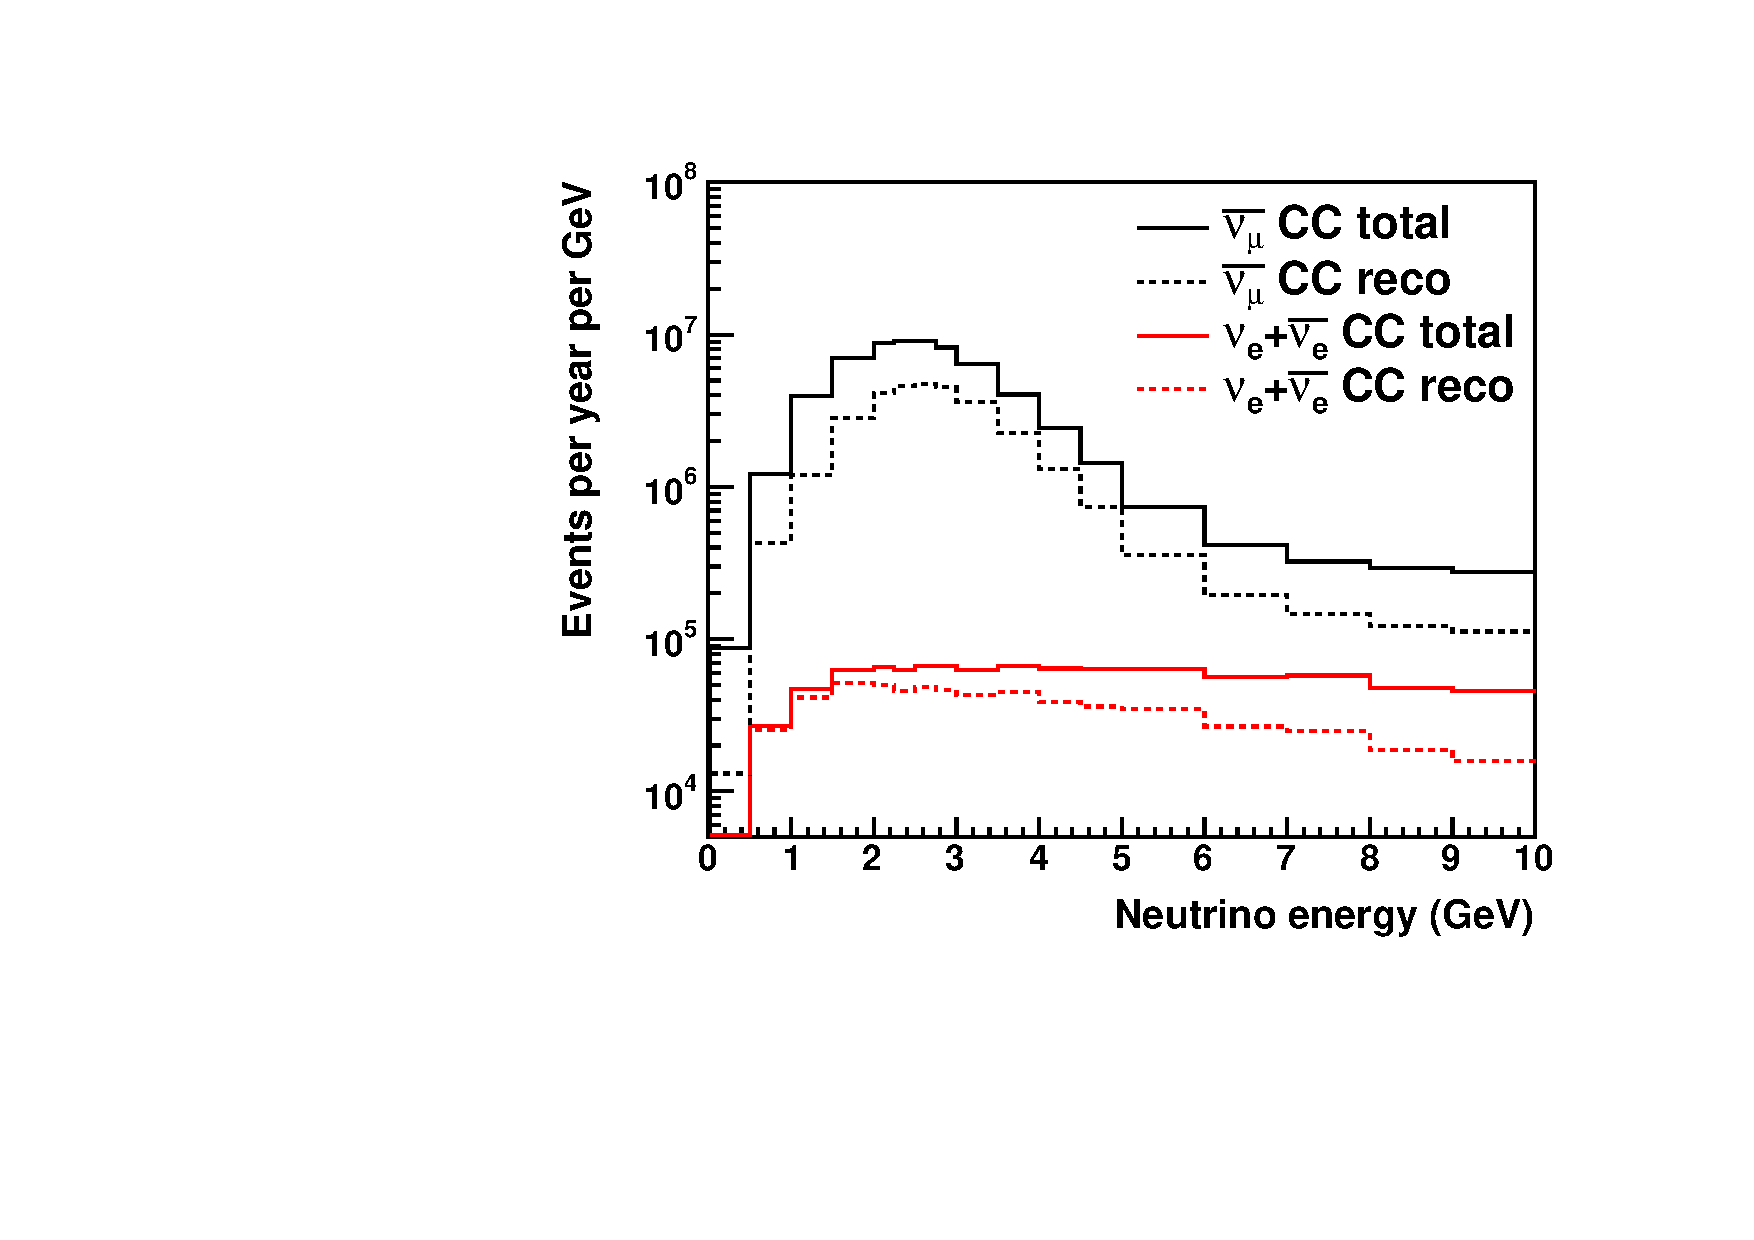
\includegraphics[width=0.48\textwidth]{graphics/lartpc/event_rate_RHC.pdf}
\end{dunefigure}

Event rates for different final states are given in Tables~\ref{tab:FHC_rates} and~\ref{tab:RHC_rates} for \dword{fhc} and \dword{rhc} beam modes, respectively. The tables are based on a simulation of GENIE version 2.12.10 with the \texttt{DefaultPlusCCMEC} physics list. The first two columns give the total rate, and the estimated number of well-reconstructed events. The second two columns give the same quantities but restricted to the oscillation region.

\begin{dunetable}
	[Event rate table FHC]
	{ccccc}
	{tab:FHC_rates}
	{\dword{fhc} Event rates in \dword{ndlar}. Accepted is defined a the $\mu$ is either contained or matched to  \dword{ndgar}, and the hadronic shower is contained (\textless\SI{30}{\mega\electronvolt} in the outermost \SI{30}{\centi\metre} of the LAr).}
	\dword{fhc} mode & total & accepted & \SIrange{0.5}{4.0}{\giga\electronvolt} & accepted \\ \toprowrule
	\dword{cc}\,$\nu_\mu$ & 8.21e+07 & 3.01e+07 & 5.88e+07 & 2.41e+07 \\ \colhline
	\dword{cc}\,$\bar{\nu_\mu}$ & 3.56e+06 & 1.47e+06 & 1.09e+06 & 5.29e+05 \\ \colhline
	\dword{nc} total & 2.76e+07 & 1.66e+07 & 1.9e+07 & 1.36e+07 \\ \colhline
	\dword{cc}\,$\nu_\mu+$\,0\,$\pi$ & 2.93e+07 & 1.57e+07 & 2.57e+07 & 1.34e+07 \\ \colhline
	\dword{cc}\,$\nu_\mu+$\,1\,$\pi^{\pm}$ & 2.04e+07 & 7.48e+06 & 1.66e+07 & 6.04e+06 \\ \colhline
	\dword{cc}\,$\nu_\mu+$\,1\,$\pi^{0}$ & 8.05e+06 & 2.85e+06 & 6.45e+06 & 2.23e+06 \\ \colhline
	\dword{cc}\,$\nu_\mu+$\,2\,$\pi$ & 1.05e+07 & 2.59e+06 & 6.86e+06 & 1.77e+06 \\ \colhline
	\dword{cc}\,$\nu_\mu+$\,3\,$\pi$ & 4.62e+06 & 7.2e+05 & 1.73e+06 & 3.78e+05 \\ \colhline
	\dword{cc}\,$\nu_\mu+$ other & 9.22e+06 & 7.44e+05 & 1.46e+06 & 3.09e+05 \\ \colhline
	\dword{cc} $\nu_{\mathrm{e}}+\bar{\nu_{\mathrm{e}}}$ & 1.43e+06 & 6.56e+05 & 4.47e+05 & 3.34e+05 \\ \colhline
	$\nu+\mathrm{e}^{-}$ & 8.39e+03 & 7.16e+03 & 5.31e+03 & 4.24e+03 \\ 
\end{dunetable}

\begin{dunetable}
	[Event rate table RHC]
	{ccccc}
	{tab:RHC_rates}
	{\dword{rhc} Event rates in ArgonCube. Accepted is defined a the $\mu$ is either contained or matched to the \dword{mpd}, and the hadronic shower is contained (\textless\SI{30}{\mega\electronvolt} in the outermost \SI{30}{\centi\metre} of the LAr)}
	\dword{rhc} mode & total & accepted & \SIrange{0.5}{4.0}{\giga\electronvolt} & accepted \\ \toprowrule
	\dword{cc}\,$\bar{\nu_\mu}$ & 2.63e+07 & 1.23e+07 & 2.01e+07 & 9.67e+06 \\ \colhline
	\dword{cc}\,$\nu_\mu$ & 1.36e+07 & 3.51e+06 & 3.13e+06 & 1.28e+06 \\ \colhline
	\dword{nc} total & 1.53e+07 & 9.33e+06 & 9.31e+06 & 7.21e+06 \\ \colhline
	\dword{cc}\,$\bar{\nu_\mu}+$\,0\,$\pi$ & 1.17e+07 & 6.67e+06 & 1.01e+07 & 5.6e+06 \\ \colhline
	\dword{cc}\,$\bar{\nu_\mu}+$\,1\,$\pi^{\pm}$ & 7.56e+06 & 3.5e+06 & 6.01e+06 & 2.73e+06 \\ \colhline
	\dword{cc}\,$\bar{\nu_\mu}+$\,1\,$\pi^{0}$ & 2.39e+06 & 9.61e+05 & 1.86e+06 & 7.19e+05 \\ \colhline
	\dword{cc}\,$\bar{\nu_\mu}+$\,2\,$\pi$ & 2.62e+06 & 8.14e+05 & 1.63e+06 & 4.99e+05 \\ \colhline
	\dword{cc}\,$\bar{\nu_\mu}+$\,3\,$\pi$ & 8.3e+05 & 1.75e+05 & 3.02e+05 & 7.53e+04 \\ \colhline
	\dword{cc}\,$\bar{\nu_\mu}+$ other & 1.16e+06 & 1.4e+05 & 1.96e+05 & 4.29e+04 \\ \colhline
	\dword{cc}\,$\nu_{\mathrm{e}}+\bar{\nu_{\mathrm{e}}}$ & 9.25e+05 & 4.01e+05 & 1.95e+05 & 1.5e+05 \\ \colhline
	$\nu+\mathrm{e}^{-}$ & 6.44e+03 & 5.75e+03 & 3.98e+03 & 3.42e+03\\
\end{dunetable}

\subsubsection{Neutrino pile-up mitigation}
\label{sec:ndlar-pileup}

The DUNE Near Detector complex requires a LArTPC design that is resilient to beam neutrino pileup, as mis-assignment of final state particles can result in mis-classification of neutrino interaction type and/or a bias in reconstructed neutrino energy. For a typical 10~$\mu$s-wide LBNF beam spill at 1.2~MW beam power, a mean of 55 neutrino interactions --- including targets both internal (57\%) and external (43\%) to the LArTPC --- produce ionization and scintillation signals within the 105~m$^3$ active volume. Optically segmenting the detector volume into 70 drift regions results in a mean of 5 scintillation signals per segment per spill. Assuming a scintillation time resolution of 25~ns, the rate of optical signal pile-up is 3\% per module per spill, relative to 30\% for a monolithic detector of equal size. With modest resolutions for both scintillation signal amplitude and position within the module, the corresponding ionization signals in each module can be accurately time-tagged and thereby associated to the correct neutrino interaction. The modular design maintains this capability after the LBNF beam power is upgraded to 2.4~MW.

The ND-LAr detector design entails a $7\times5$ modular array. Each module is 3~m high, 1~m long, 1~m wide and comprised of two TPC drift regions separated by a central cathode plane, each with maximum drift length of 50~cm. Each drift region is optically isolated and independently instrumented for scintillation light detection. This ND-LAr modular design is compared to a far detector-like LArTPC with a central cathode and two drift regions to assess the benefit of modularity relative to a "monolithic" LArTPC design. The same instrumented (active) LAr volume and bounding dimensions (5~m $\times$ 7~m $\times$ 3 m) is assumed between modular and monolithic schemes for direct comparisons. The simulation sample used in this study was constructed with LBNF-like neutrino fluxes input into a GENIE neutrino interaction model. The LBNF beam spill microstructure entails six batches each comprised of 84 53.1 MHz bunches. One thousand LBNF-like beam spills were simulated at 1.2 MW beam power and propagated through the ND hall detector geometry including the surrounding rock using a Geant4 simulation. Deposited energy was calculated by the summation of visible energy depositions in the ND-LAr active volume.

Assuming a 1 MeV threshold for a single visible interaction per TPC, modularity alone reduces the ambiguity in single neutrino interaction selection by a factor of $\approx7$. This 1~MeV visible interaction threshold per TPC has sub-percent level bias on visible energy for neutrino interactions with neutrino vertex residing within the charge instrumented volume and visible energy ex- ceeding 500 MeV.
With roughly 55 independent neutrino interactions producing visible signals per 10~$\mu$s spill, the chance of two interactions being close in time is relatively frequent. The ND-LAr technical requirements call for scintillation light timing resolution of 20 ns. This specification assumes late scintillation light can be effectively subtracted from the prompt component. Scintillation light pileup is mitigated with modularity. Even at a relatively modest timing resolution of 200~ns, a factor of 4 improvement in individual interaction light identification is gained with the described modularity. At 25~ns timing resolution, 3\% of neutrino interactions within a TPC are within 25~ns of each other with the current modular TPC scheme, whereas 30\% of neutrino interactions are within 25~ns of each other with a monolithic TPC scheme. These results are shown in Figure \ref{fig:ndlar-ana-pileup}.

Note that this comparison does not take into account interactions outside the charge instrumented volume. The monolithic TPC scheme would have sensitivity to light signals from these interactions, as opposed to the modular scheme which would not owing to the light-tight modules. Thus, charge-light signal combinatorics are further complicated in the monolithic TPC design, resulting in an underdetermined linear system.

\begin{figure}
\centering
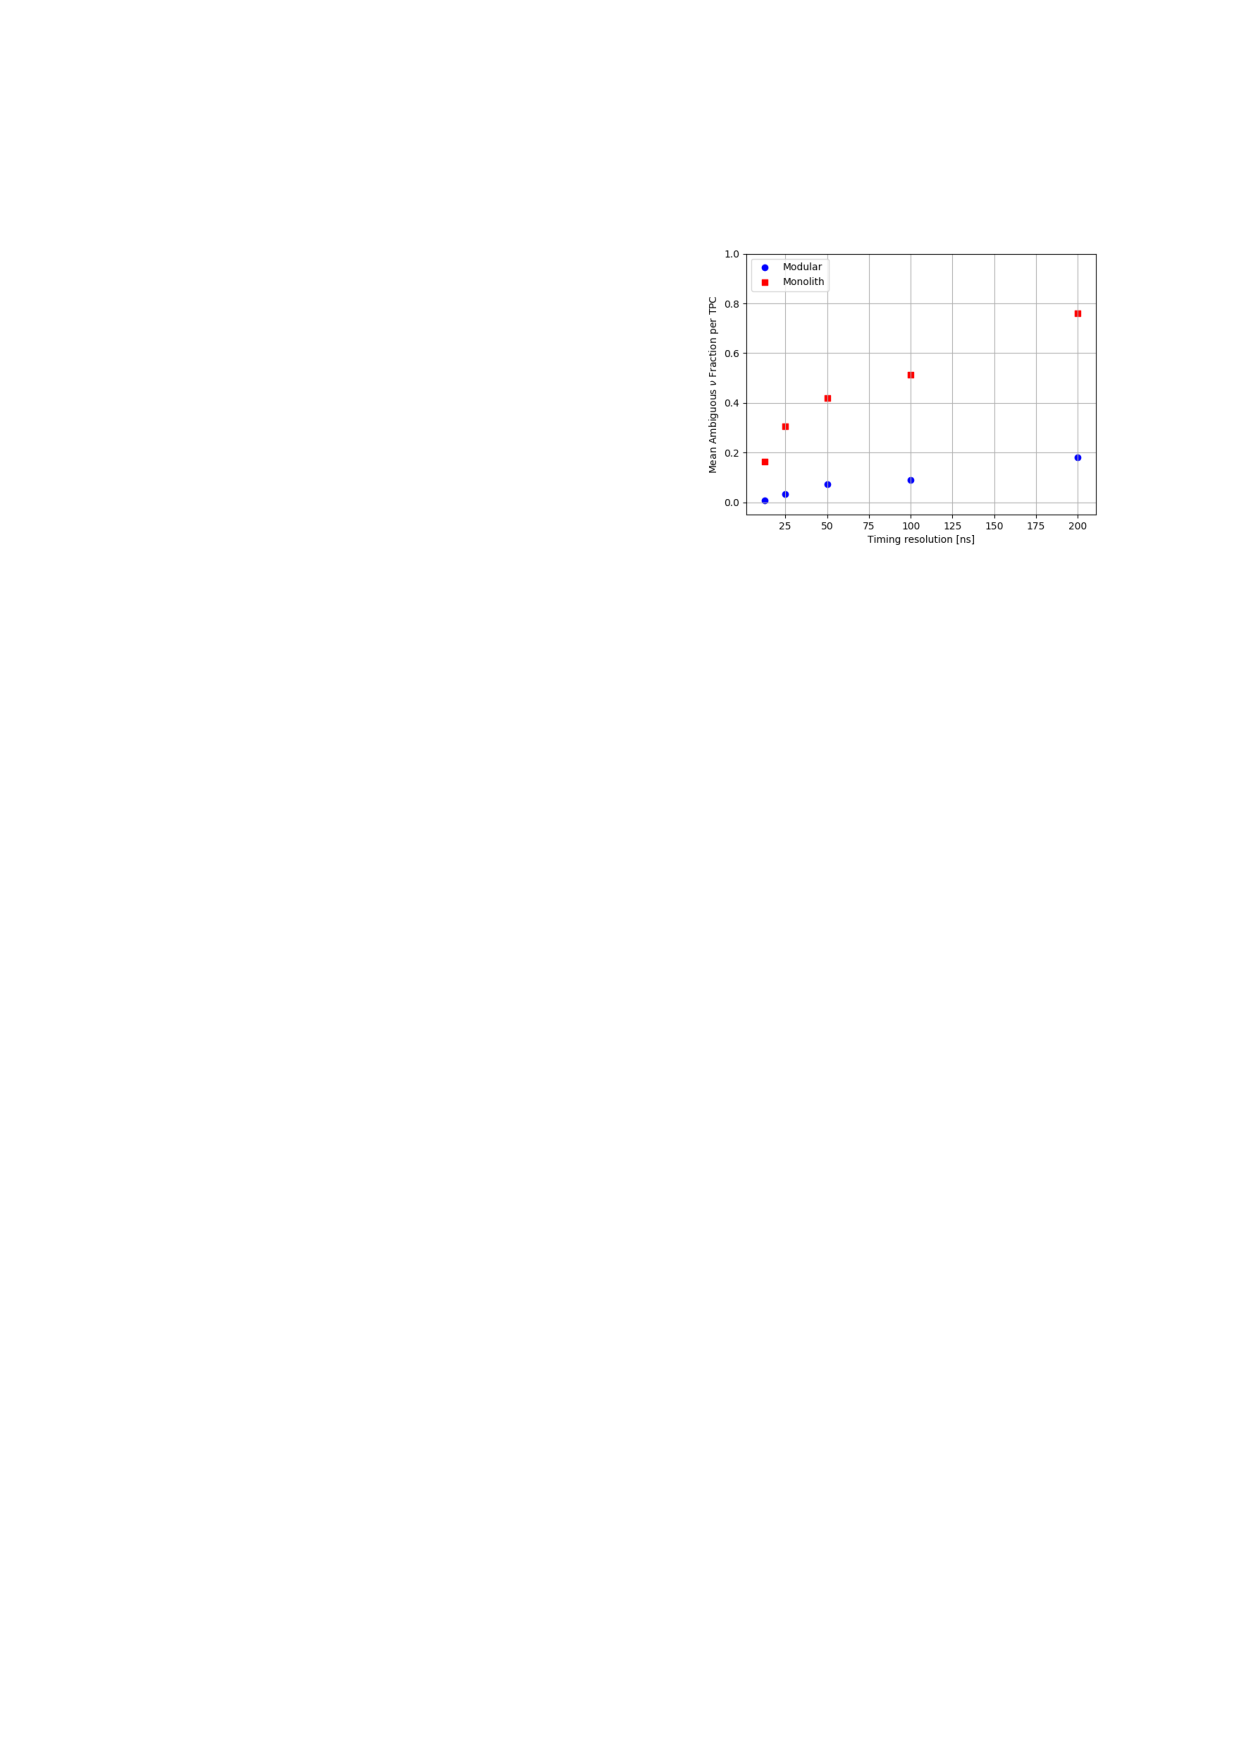
\includegraphics[width=0.5\textwidth]{pileup_ambiguous_nu.pdf}
\caption{Assuming removal of late scintillation light from the prompt component, the ``ambiguous $\nu$ fraction'' reflects the fraction of neutrino interactions per TPC drift region that cannot be resolved for a given timing resolution.}
\label{fig:ndlar-ana-pileup}
\end{figure}

{\it Figure: Signal hit clustering efficiency/purity after pileup rejection.}

\subsubsection{Detector acceptance \textcolor{red}{from CDR}}

%Detector acceptance with $\mu$ and hadronic containment requirements. Per CDR, with additional details on $\mu$ and clustering efficiency from ML reco folded in.
%
%{\it Figure: Detector acceptance vs. neutrino interaction kinematics: muon reconstruction.}
%{\it Figure: Detector acceptance vs. neutrino interaction kinematics: hadronic containment.}

Muons are considered as useful for physics if they stop in the active region of \dword{arcube} or if they leave the \dword{lar} detector and are reconstructed in a magnetic spectrometer downstream.  
Under the assumption that the downstream magnetic spectrometer is the multi-purpose detector, Figure~\ref{fig:ndlar-ana-muonacc}  shows the muon acceptance as a function of true neutrino energy (on the left) and muon energy (on the right). 
The acceptance dip at \SI{1}{\giga\electronvolt} in muon energy is from muons that exit \dword{arcube} and are not reconstructed in the \dword{mpd} downstream. This dip can be reduced by minimizing the passive material between the liquid argon and high pressure gaseous argon detectors.

\dword{icarus} and \dword{microboone} have used multiple Coulomb scattering to determine muon momentum \cite{Abratenko:2017nki}.  
This technique may prove to be useful for muons in \dword{arcube} and could  mitigate somewhat the size of the dip in Figure~\ref{fig:ndlar-ana-muonacc}.   

\begin{dunefigure}[Muon acceptance as a function of true neutrino energy and true muon energy]{fig:ndlar-ana-muonacc}
{Muon acceptance shown as a function of true neutrino energy (left) and true muon energy (right).  The acceptance for muons that stop in \dword{arcube} is shown in red and that for muons reconstructed in the downstream magnetic spectrometer is shown in blue.}
      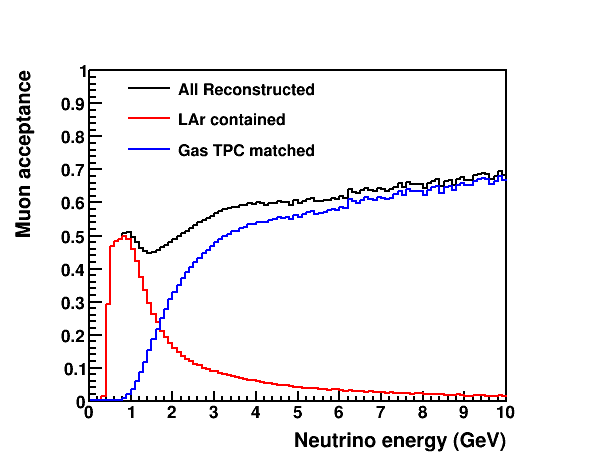
\includegraphics[width=0.45\textwidth]{graphics/lartpc/muReco_Ev.png}
      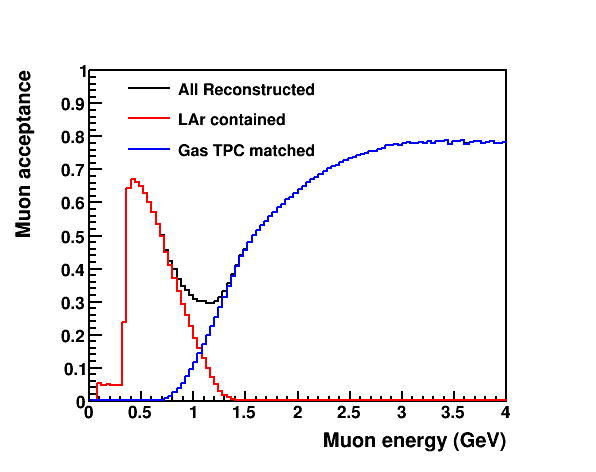
\includegraphics[width=0.45\textwidth]{graphics/lartpc/muReco_Emu.png}
\end{dunefigure}

\paragraph{Acceptance vs.\ energy and momentum transfer}

The acceptance of \dword{arcube} with the \dword{mpd} acting as a downstream spectrometer can be studied in a more nuanced way by looking at it as a function of the energy $q_0$ and three-momentum $q_3$ transferred to the target nucleus. 
The energy transfer is simply $q_0=E_\nu - E_\mu$. 
The three-momentum transfer is related to the four-momentum transfer $Q$ and $q_0$ by $q_3 = \sqrt{Q^2 + q_0^2}$. 
These variables have long been used to study nuclear structure in electron scattering experiments. 

\begin{dunefigure}[Neutrino acceptance as a function of energy and momentum transfer]{fig:ndlar-ana-q0q3acc}
{Neutrino acceptance shown as a function of energy transfer and momentum transfer ($q_0$ and $q_3$) to the target nucleus. The units for $q_0$ and $q_3$ are \SI{}{\giga\electronvolt} and \SI{}{\giga\electronvolt}/c, respectively. The figures show the event rate (left) and the acceptance (right) for reconstructing the muon and containing the hadronic system. The top row was made for neutrinos with true neutrino energy between \SIrange{1.0}{2.0}{\giga\electronvolt} and the bottom was made for neutrinos between \SIrange{4.0}{5.0}{\giga\electronvolt}.}
      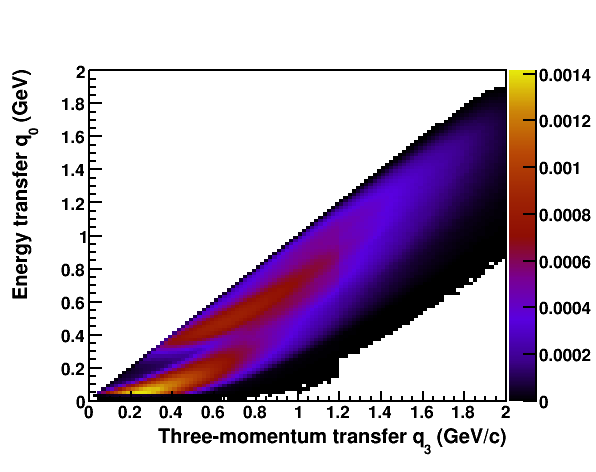
\includegraphics[width=0.45\textwidth]{graphics/lartpc/rate_q0q3_Ev_1000_2000.png}
      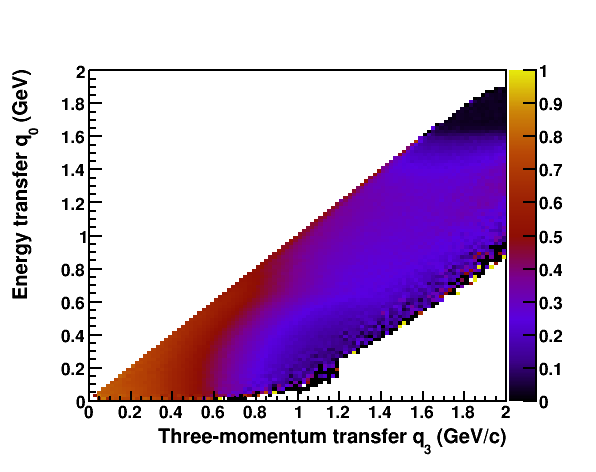
\includegraphics[width=0.45\textwidth]{graphics/lartpc/eff_q0q3_Ev_1000_2000.png}
      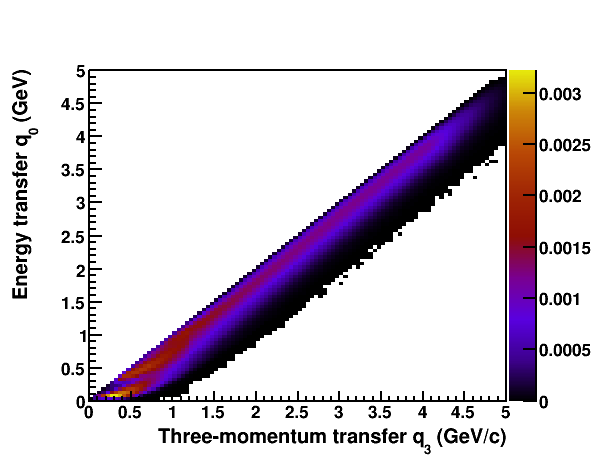
\includegraphics[width=0.45\textwidth]{graphics/lartpc/rate_q0q3_Ev_4000_5000.png}
      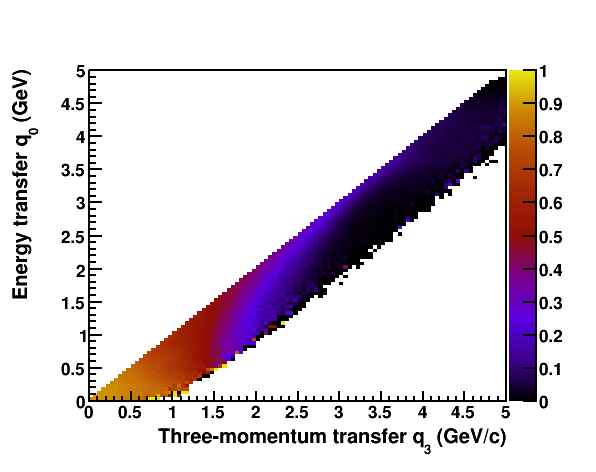
\includegraphics[width=0.45\textwidth]{graphics/lartpc/eff_q0q3_Ev_4000_5000.png}
\end{dunefigure}

Figure~\ref{fig:ndlar-ana-q0q3acc} shows the event rate (left figures) and acceptance (right figures) in bins of $(q_3,q_0)$.
The rows correspond to two neutrino energy bins.	
The top row is for $E_\nu$ between \SIrange{1.0}{2.0}{\giga\electronvolt} and it covers the first oscillation maximum. 
The second bin is for $E_\nu$ between \SIrange{4.0}{5.0}{\giga\electronvolt}.  
The rate histograms have ``islands''  corresponding to hadronic systems with fixed invariant mass. 
The islands are smeared by Fermi motion and decay width. 
The lower island in $(q_3,q_0)$ corresponds to the quasi-elastic peak while the upper corresponds to the $\Delta$ resonance. 
One should note that the axes in the lower row cover a larger range of kinematic space than those in the upper row. 

The acceptance is generally very good in the kinematic region where the vast majority of the events occur but is nowhere perfect. 
This is not necessarily a problem because the loss is chiefly geometrical. 
Losses typically occur in events with a vertex near one boundary of the detector where the muon, or hadronic system exits out that boundary.  
However for each lost event there is generally a set of symmetric events that are accepted because the final state is rotated by some angle about the neutrino beam axis ($\phi$ symmetry) or is closer to the centre of the fiducial volume (x,y symmetry).

Regions where the acceptance is zero are problematic because they will introduce model dependence into the prediction of the rate at the far detector (which has a nearly $4\pi$ acceptance). 
Acceptances of even a few \% in some kinematic regions are not necessarily a problem as long as the event rate is large enough to accumulate a statistically significant number of events.
There is a potential danger if the acceptance varies quickly as a function of the kinematic variables because a small mismodeling of the detector boundaries or neutrino cross-sections could translate into a large mismodeling in the number of accepted events. 

The size of the accepted event set decreases as a function of both $q_0$ and $q_3$ (and therefore $E_\nu$) due to more energetic hadronic systems and larger angle muons. 
This can clearly be seen in the transition from the colored region to the black region in the $\SI{4.0}{\giga\electronvolt} < E_\nu < \SI{5.0}{\giga\electronvolt}$ acceptance histogram shown in the lower right-hand corner of Figure~\ref{fig:ndlar-ana-q0q3acc}. The transition is smooth and gradual.

The acceptance for $\SI{1.0}{\giga\electronvolt} < E_\nu < \SI{2.0}{\giga\electronvolt}$ (shown in the upper right-hand corner of Figure~\ref{fig:ndlar-ana-q0q3acc}) is larger than 10\% except in a small region at high $q_0$ and $q_3$. 
Events in that region have a low-energy muon and are misidentified as neutral-current according to the simple event selection applied in the study. 
The fraction of events in that region is quite small, as can be seen in the upper left-hand plot of Figure~\ref{fig:ndlar-ana-q0q3acc}. 

\begin{figure}
\centering
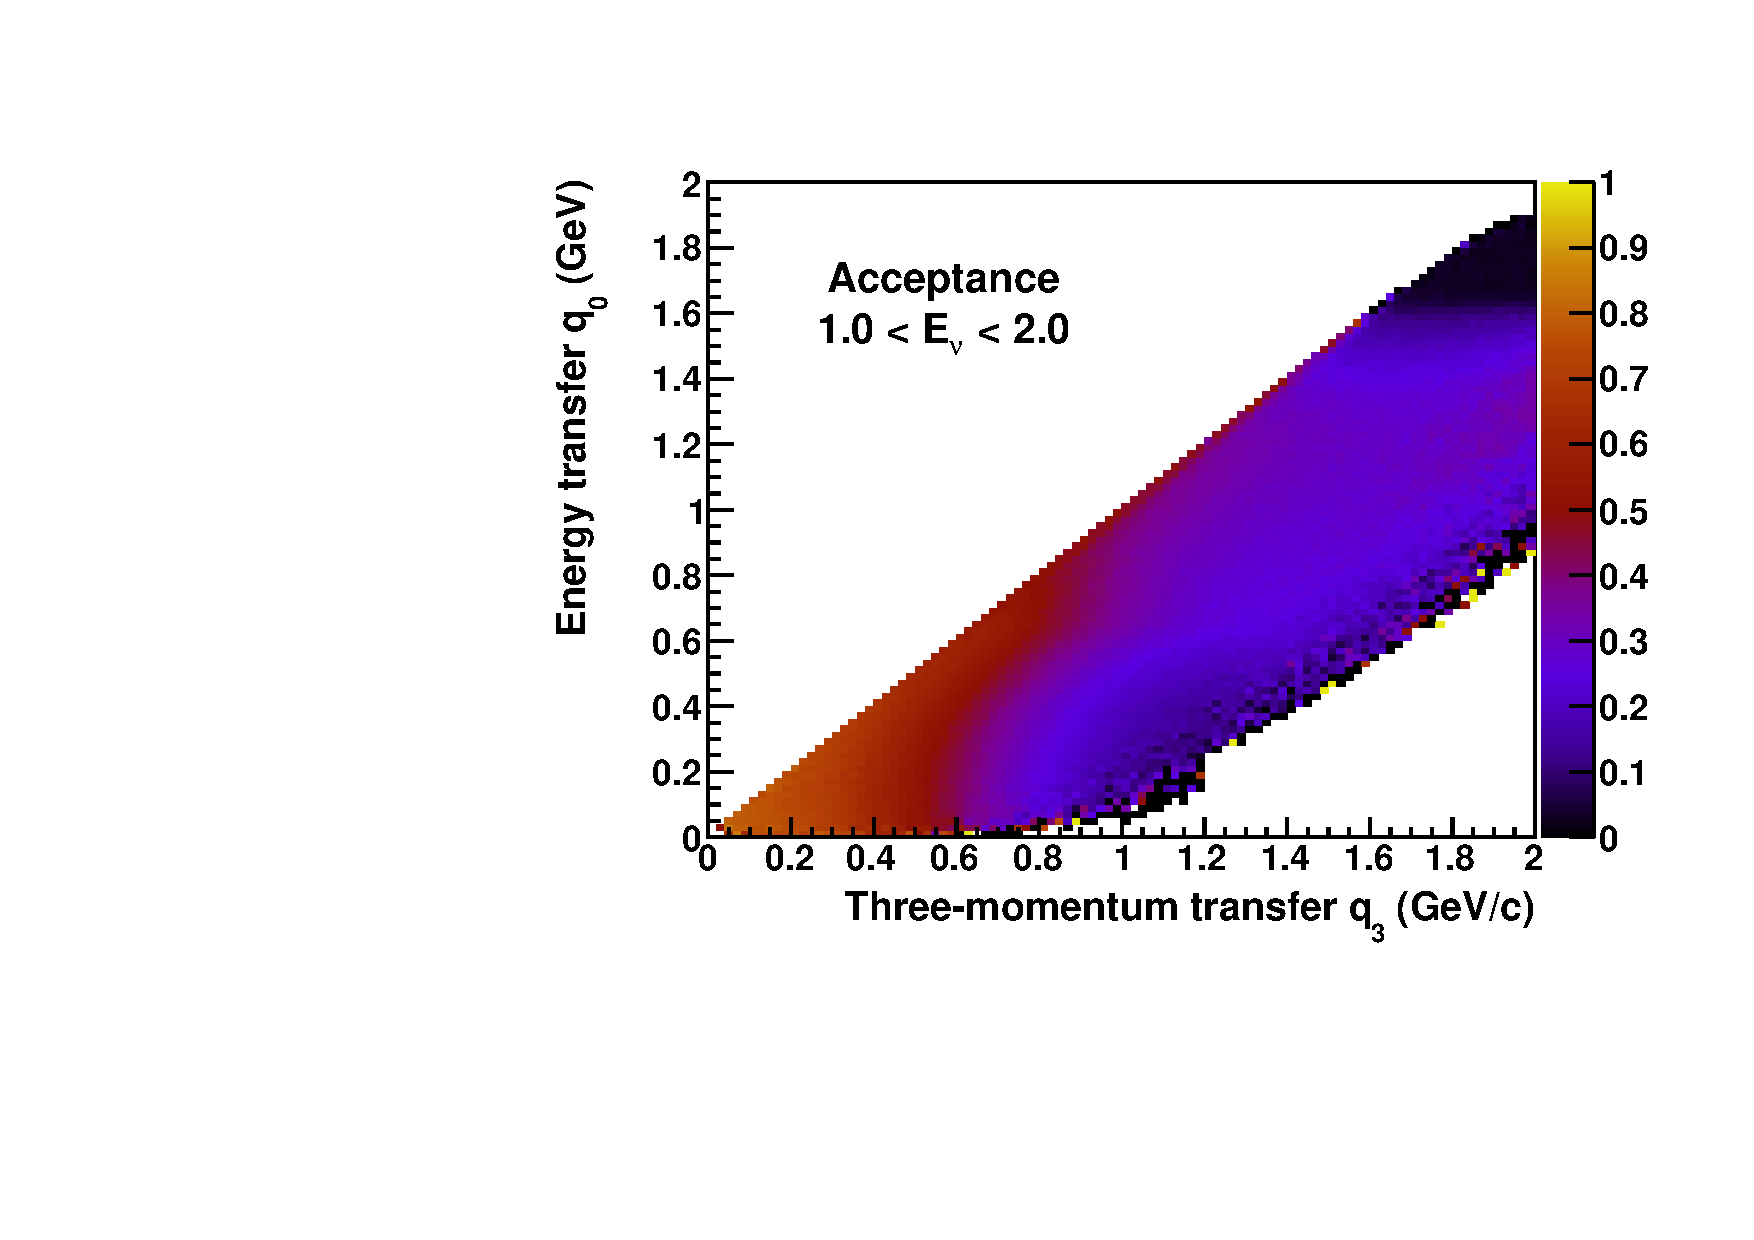
\includegraphics[width=0.49\textwidth]{graphics/lartpc/eff_q0q3_Ev_1000_2000.pdf}
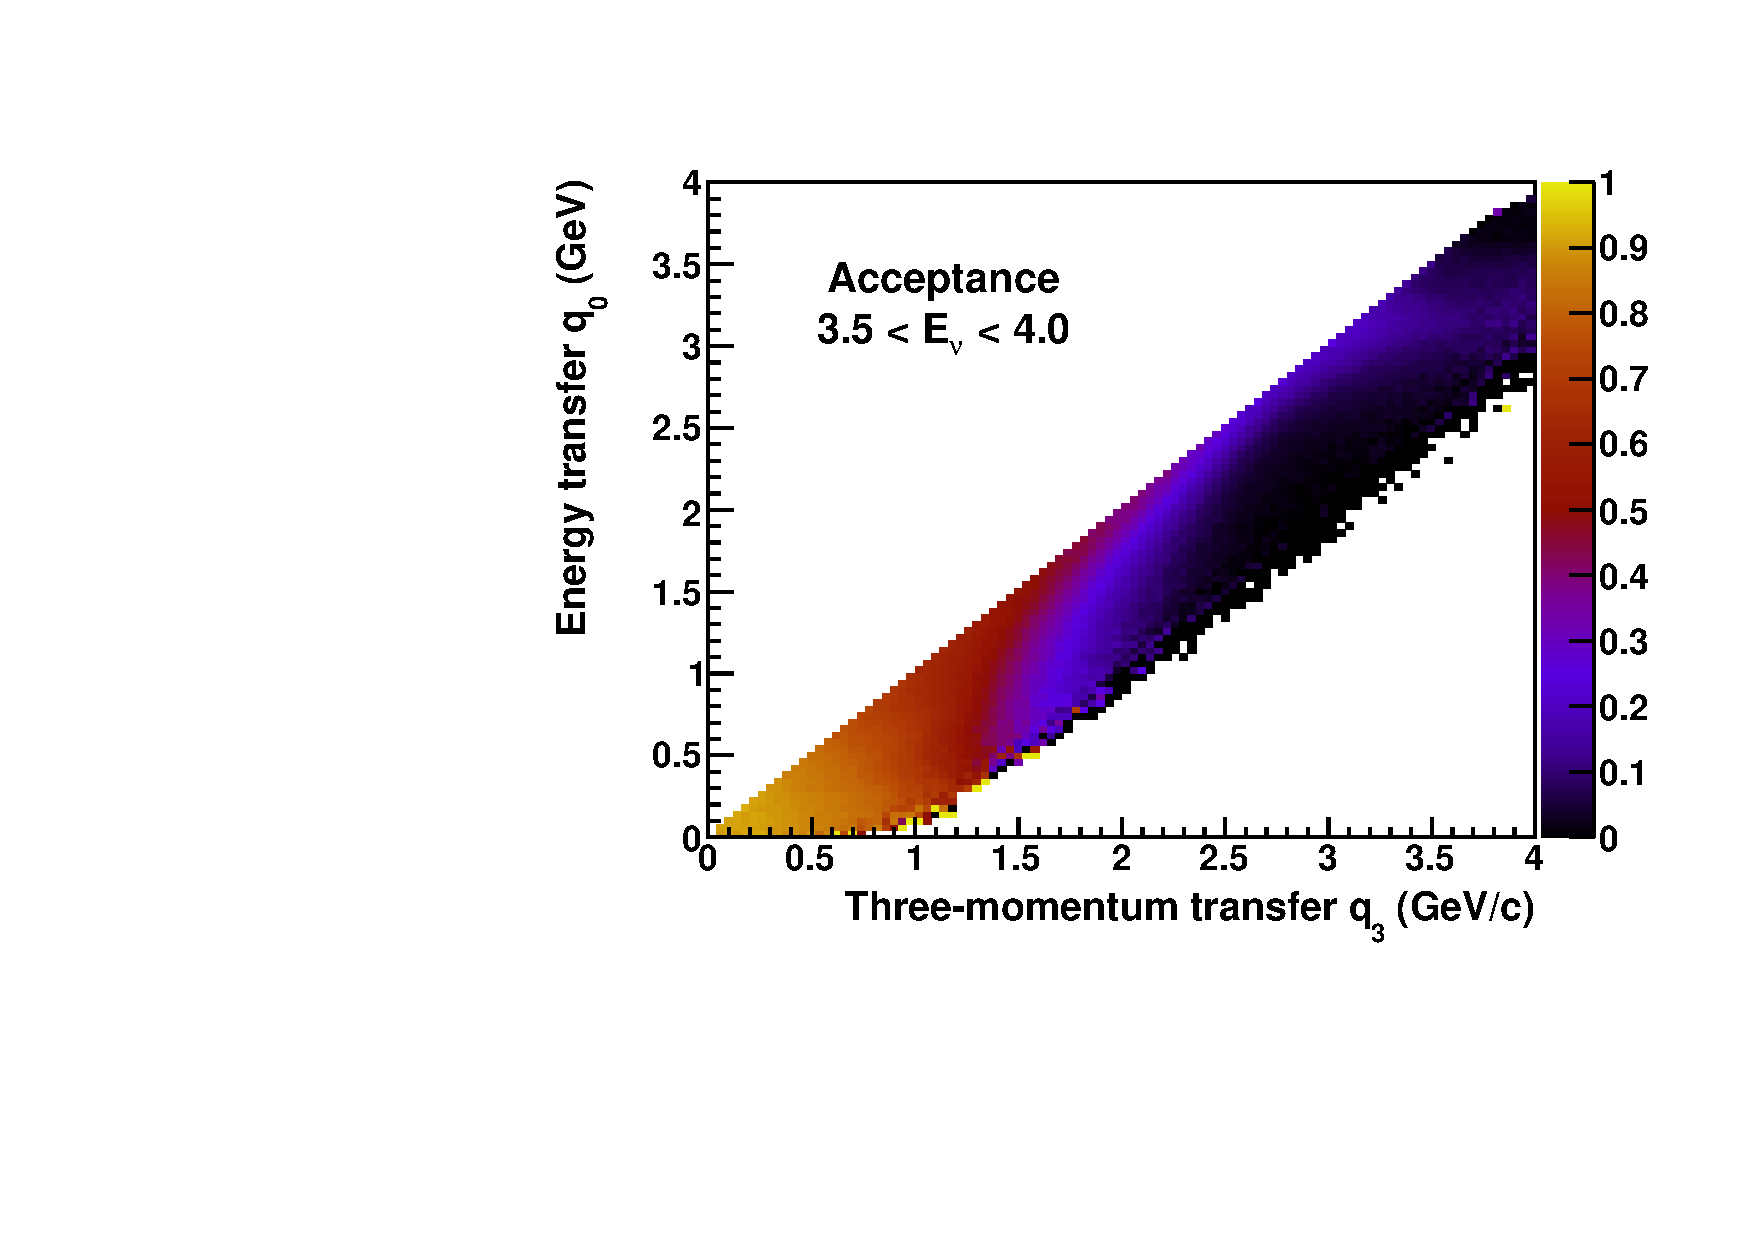
\includegraphics[width=0.49\textwidth]{graphics/lartpc/eff_q0q3_Ev_3500_4000.pdf}
\caption{Neutrino acceptance as a function of energy and momentum transfer}
{Neutrino acceptance shown as a function of energy transfer and momentum transfer ($q_0$ and $q_3$) to the target nucleus. The units for $q_0$ and $q_3$ are \SI{}{\giga\electronvolt} and \SI{}{\giga\electronvolt}/c, respectively.}
\label{fig:q0q3acc}
\end{figure}

\subsubsection{Event reconstruction performance}

The ND-LAr reconstruction is handled using two methods: a realistic parametric response function applied to simulated final-state particle trajectories, and a complete event clustering and topological reconstruction based on Deep Learning techniques. In both cases, neutrino interactions are simulated using the GENIE v2.12.10 neutrino event generator and a detailed geometry including the full Near Detector hall and the surrounding rock environment, with final state particle tracking using the Geant4-based edep-sim package. This simulation includes particle scattering and energy losses in inactive regions of the ND-LAr detector modules.

The parametric reconstruction is used for high-level physics studies pending their implementation in the full reconstruction. This data-driven model includes a calorimetric hadronic energy reconstruction, accounting for contamination due to neutrino event pile-up by adding up to 500 MeV to the calorimetric energy for 10\% of interactions; studies of neutrino pile-up disambiguation shown above indicate that this is a conservative overestimate of this effect. Neutral pions may be mis-reconstructed as electron events, when one $\gamma$ Compton scatters near the vertex and the other is low-energy ($p<50$~MeV) and/or collinear (within 10~mrad). Electrons are not charge-tagged, and the efficiency is parameterized as linear with a threshold at 300 MeV, and 100\% above 700 MeV. An energy-dependent probability models mis-reconstruction of CC electron events as NC interactions. For reconstructed CC electrons, an energy-dependent electromagnetic shower energy resolution of $0.03+0.1/\sqrt{E}$ GeV is applied as well as a smearing of the angle with respect to the incoming neutrino direction. Muon momentum reconstruction for fully-contained tracks is range-based, with an energy resolution of 5\% for tracks $>100$~cm in length and an analytic smearing of the reconstructed angle. Charge tagging is assumed to be 100\% effective for the FHC beam mode; in the RHC mode a tag based on Michel electrons is 75\% efficient, with a 25\%$\times$75\% probability to mis-tag a $\mu^-$ as a $\mu^+$.

The Deep Learning based reconstruction is a novel approach to reconstructing the fully 3D information available from the LArPix TPC readout, and builds on earlier work in wire-based LArTPCs including MicroBooNE (cite) and ProtoDUNE-SP (cite). The input to the reconstruction is a set of ``hit'' detector voxels, a small volume corresponding to the pixel area and charge integration $\Delta t$ for all triggered readout channels in an event. The output is a reconstructed interaction, with these voxels grouped and labeled with a particle type, and organized into a particle flow hierarchy. The reconstruction is performed in several stages:
\begin{enumerate}
\item Particle type identification: Labeling of voxels according to particle type, i.e. as minimally (highly) ionizing particles, or mips (hips), showers, $\delta$ rays, or Michel electrons. The PID labeling on neutrino-like events is $>98$\% correct for hips, mips, and showers, and $>90$ correct for $\delta$ rays and Michel electrons \cite{domine2020point}.
\item Dense clustering: Grouping of high-density regions of voxels into track-like clusters. This stage achieves 98.7\% efficiency and 99.1\% purity on neutrino-like simulation samples \cite{koh2020scalable}.
\item Shower clustering: Grouping of low-density regions of voxels into shower-like clusters. This stage achieves 99.5\% efficiency and 99.6\% purity on neutrino-like simulation samples \cite{koh2020scalable}.
\item Interaction grouping: Connecting and grouping of sets of track- and shower-like clusters into individual neutrino (or other particle) interactions. This stage achieves an average 98.4\% efficiency and 99.8\% purity on neutrino-like simulation samples with $\sim10$ interactions \cite{koh2020scalable}.
\item Particle identification: Identification of the track- and shower-like clusters within their interaction context with specific particle types, e.g. two photons associated with a $\pi^0$, or a $\mu^-$ decaying into a Michel electron.
\item Particle flow: Assembly of all particles within an interaction into a hierarchy representing the sequence of interactions and decays following from the primary interaction.
\end{enumerate}
An initial selection of $\pi^0\to\gamma\gamma$ decays has been developed based on this framework to provide a ``standard candle'' for electromagnetic energy calibration and develop shower reconstruction tools. Figure \ref{fig:ndlar-ana-pi0-reco} shows the reconstructed $\pi^0$ mass for an idealized detector response, and before corrections to individual shower energies to account for e.g. thresholding effects.
\begin{figure}
\centering
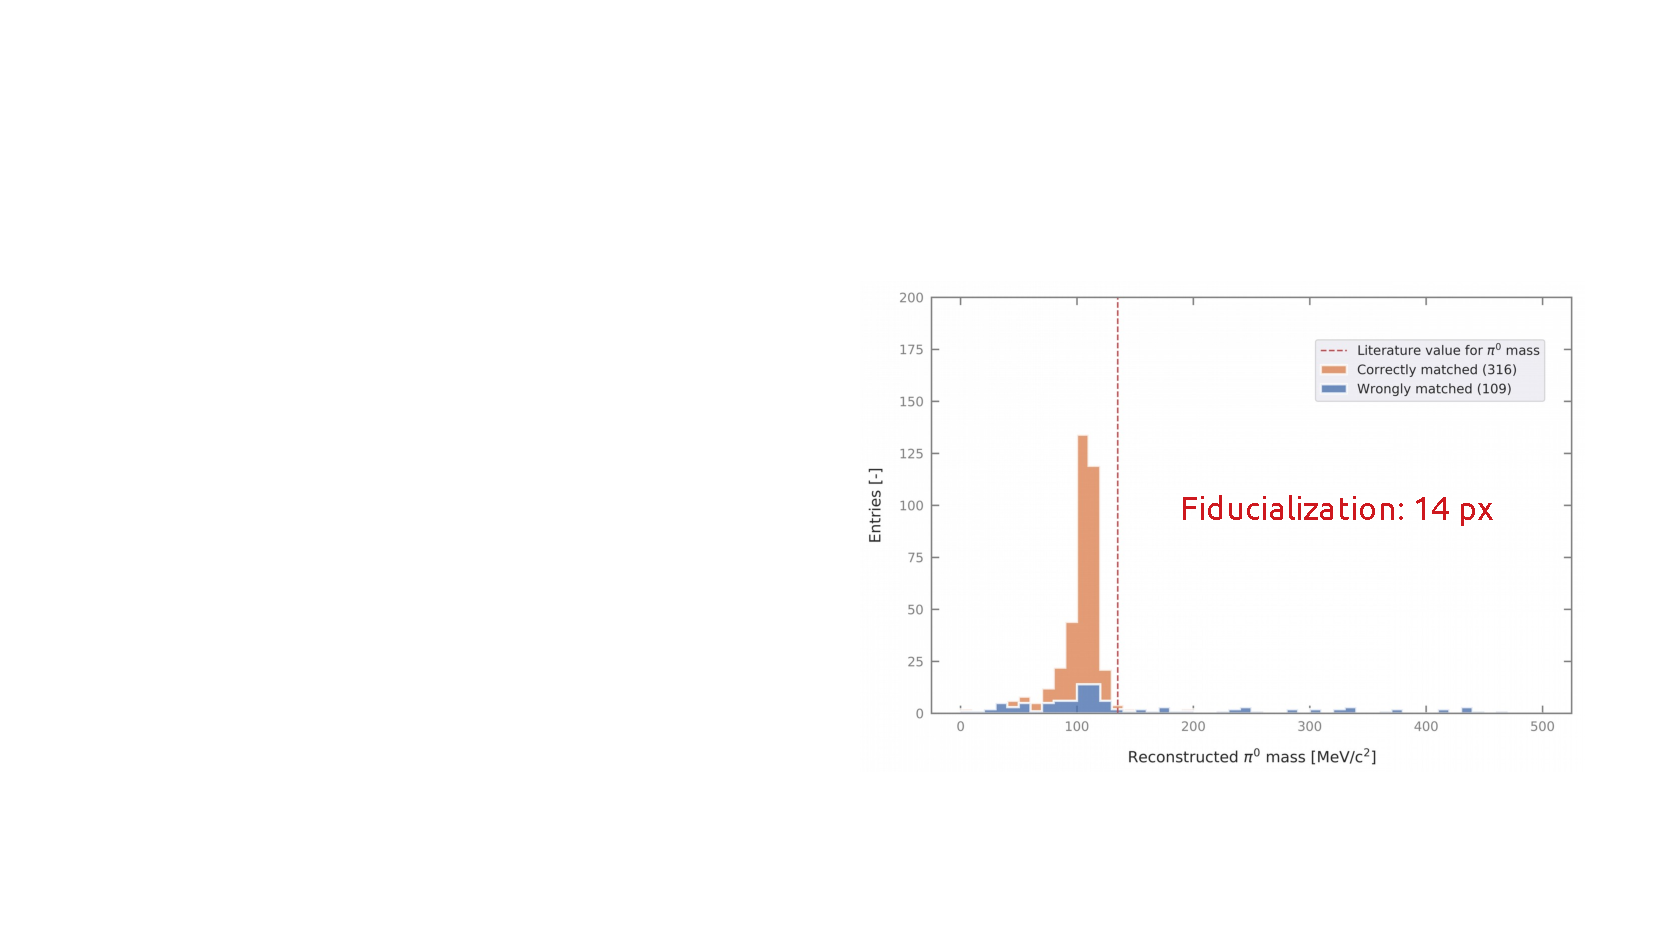
\includegraphics[width=0.5\textwidth]{pi0-reco.pdf}
\caption{Reconstructed $\pi^0$ mass before thresholding corrections, utilizing the full Deep Learning based reconstruction framework.}
\label{fig:ndlar-ana-pi0-reco}
\end{figure}

%\begin{itemize}
%    \item Energy reconstruction
%    \item Flavor/sign accuracy
%    \item Exclusive selection accuracy (muon ID efficiency, pi+ ID, pi0 ID, nu+e)
%\end{itemize}

%{\it Figure: Reconstructed vs. true neutrino energy for $\nu_\mu$CC.}
%{\it Table: Particle ID performance for ML reco}

%%%%%%%%%%%%%%%%%%%%%%%%%%%%%%%%
\section{System Design}
\label{sec:lartpc-des}
%{\it Jonathan, 1-2 pages}

\begin{itemize}
    \item 1 m by 1 m by 3 m tall TPC Module is the basic unit of ND LArTPC
    \item Each TPC module consists of a fully-functioning TPC with central cathode and two horizontal drift regions
    \item Pixelated charge readout tiles cover two anodes
    \item Light traps (two styles) cover vertical field cage walls, funnel light to SiPMs located near anode.
    \item Top and bottom of TPC module field cage is perforated, side walls are sealed.  Purified LAr is injected at top of module (below weir), exits module at bottom into cryostat bath.
\end{itemize}

{\it Figure: Exploded CAD view of TPC module, with subsystem labels}

%%%%%%%%%%%%%%% One subsection for each WBS element:
\subsection{Field Structures}
\label{sec:lartpc-des-fieldstruc}
%{\it Francois, 3 pages}

\subsubsection{Overview}
\label{sec:lartpc-fs-ovvw}
The field-shaping structure in a DUNE ND-LAr TPC module is used to define a uniform electrostatic field in the liquid argon volume in order to transport ionization electrons -- from their point of creation to the readout pixels on the anode -- without significant distortions. It must achieve a field non-uniformity $<1\,\%$ in the entirety of the active volume and operate reliably under nominal fields of $250\,$V$/$cm and peak fields of up to $500\,$V$/$cm. The footprint of the system has to be minimized in order to optimize the fraction of active volume in the detector as a whole. Additionally, this subsystem should not exceed a local heat density of $100\,$ mW/cm$^2$, which is the typical heat density of electronics used in wire-based LArTPCs~\cite{notsure} and limits liquid argon boiloff.
\subsubsection{Field Structure Key Requirements}
\label{sec:lartpc-fs-req}
The key driving design requirements and performance requirements for the field structure are summarized in Figure~\ref{fig:lartpcfsreq}. 
\begin{figure}
\centering 
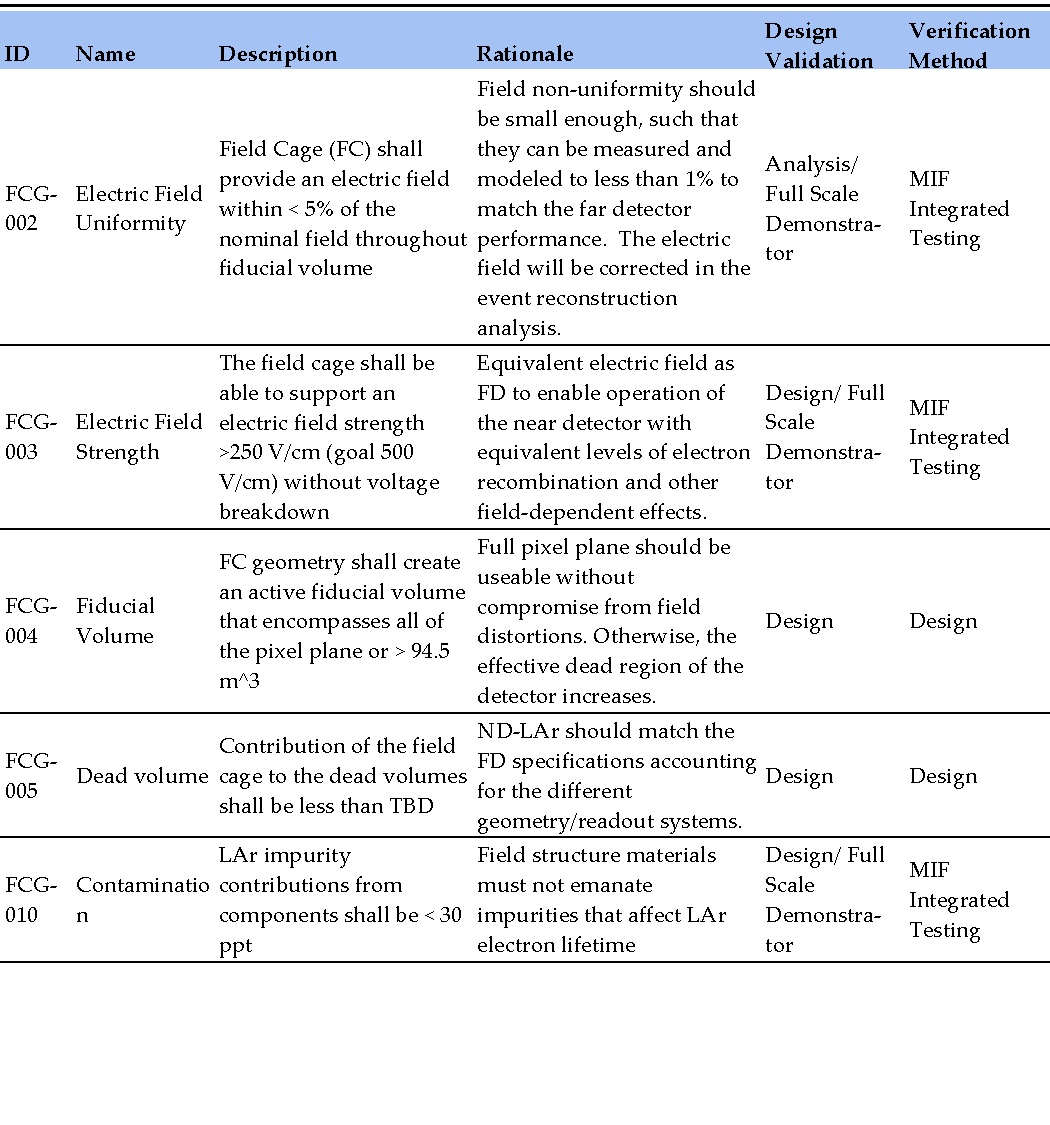
\includegraphics[width=1\linewidth]{graphics/lartpc/0Req/NDFCreqs1.pdf}
\caption{\label{fig:lartpcfsreq} ND LArTPC Key Field Structure Requirements}
\end{figure}

\subsubsection{Field Structure Design}
\label{sec:lartpc-fs-design}
Figure\,\ref{fig:field_shell} shows schematics of the field-shaping structure as a whole. It is composed of five copper-clad, 6\,mm-thick FR4 panels covered with Dupont Kapton sheets loaded with electroconductive carbon black. The central panel in the figure is the cathode -- which splits the TPC module into two optically-isolated drift volumes and sets the maximum potential -- while the other four form the `field shell': a resistive structure which continuously decreases the voltage from the cathode to the grounded anode. The bottom and top panels of the field shell are perforated with $\sim350$ 4\,mm holes to facilitate liquid argon circulation. This approach to field-shaping has several advantages over a traditional TPC field cage:
\begin{itemize}
  \item it extends the achievable active volume by having a smaller the footprint but also by reducing local field non-uniformity created by field-shaping rings;
  \item the resistive heating is spread over entire panels instead of being localized on the surface of resistors, which drastically stifles liquid argon nucleation;
  \item it does not suffer from single points of failure, as the whole panel drives the resistance;
  \item the field does not spike around rings, considerably reducing the risk of arcing.
\end{itemize}
The field-shaping structure also provides mechanical support for the entire TPC module.

\begin{figure}[htbp]
\centering
\begin{minipage}[b]{.4\textwidth}

\includegraphics[width=\linewidth]{graphics/lartpc/FieldCage/fc2.PNG}
\end{minipage}
\qquad
\begin{minipage}[b]{.4\textwidth}
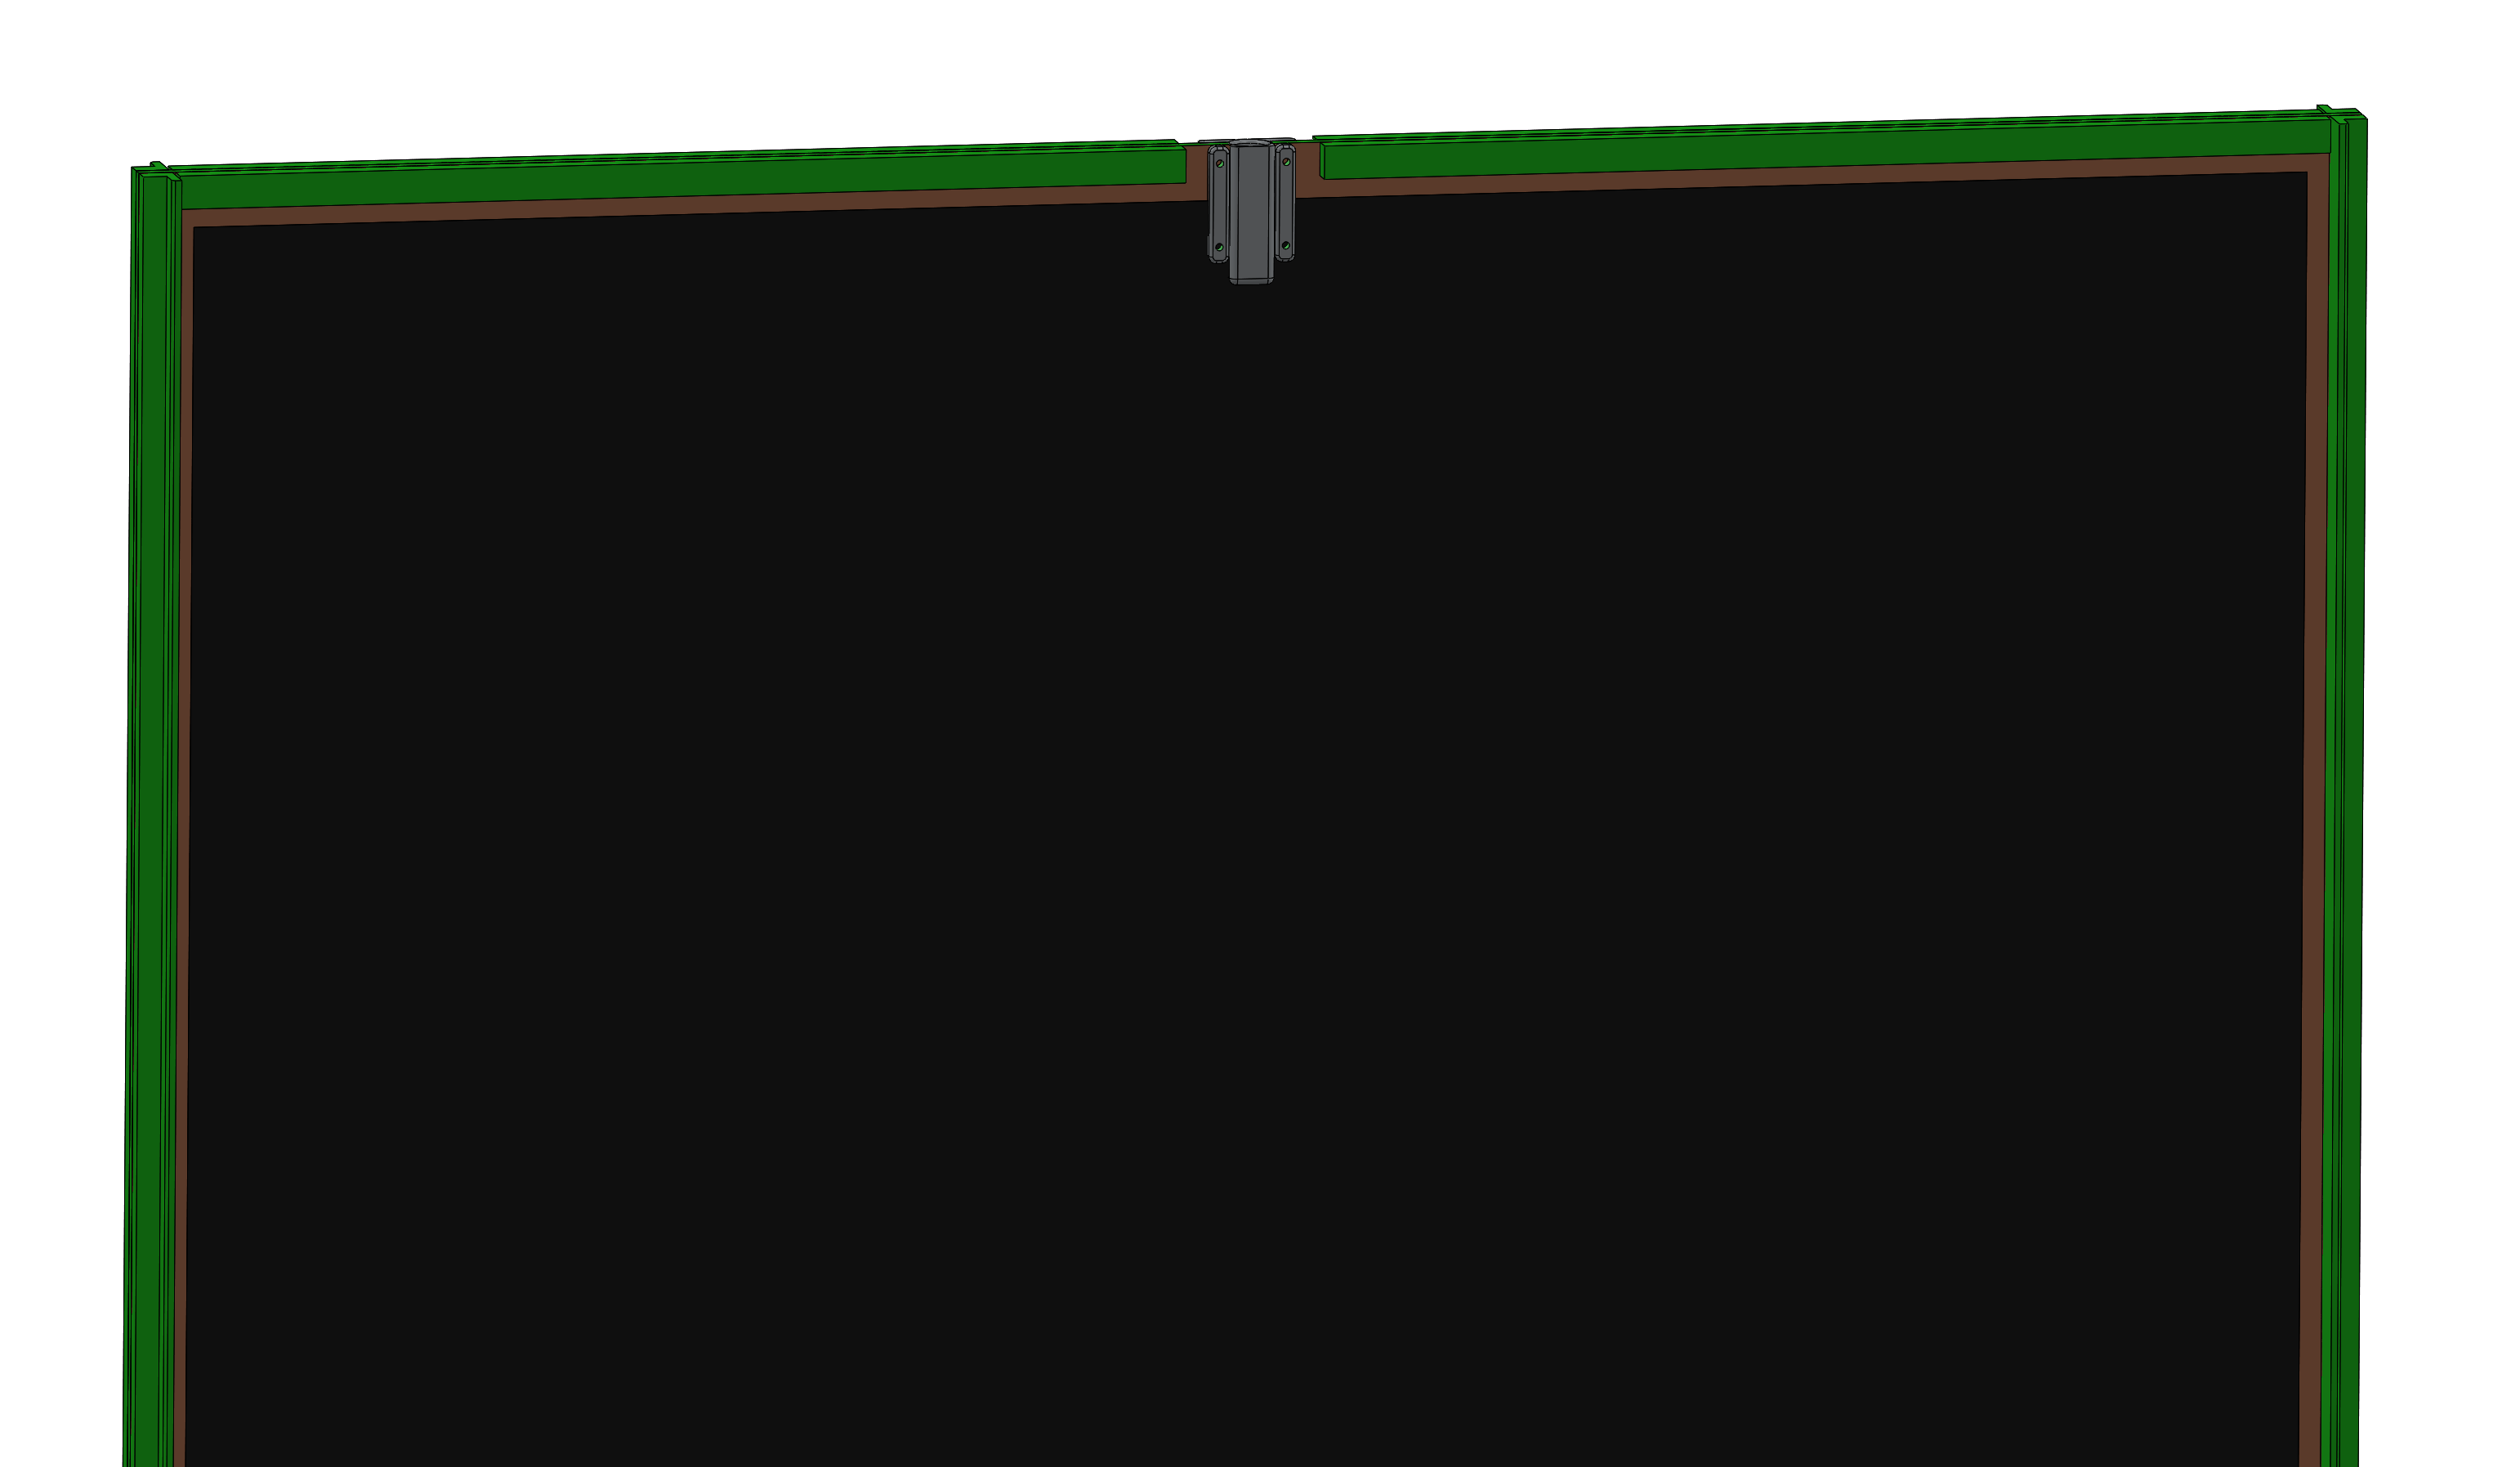
\includegraphics[width=\linewidth]{graphics/lartpc/FieldCage/cathodeandhv.PNG}
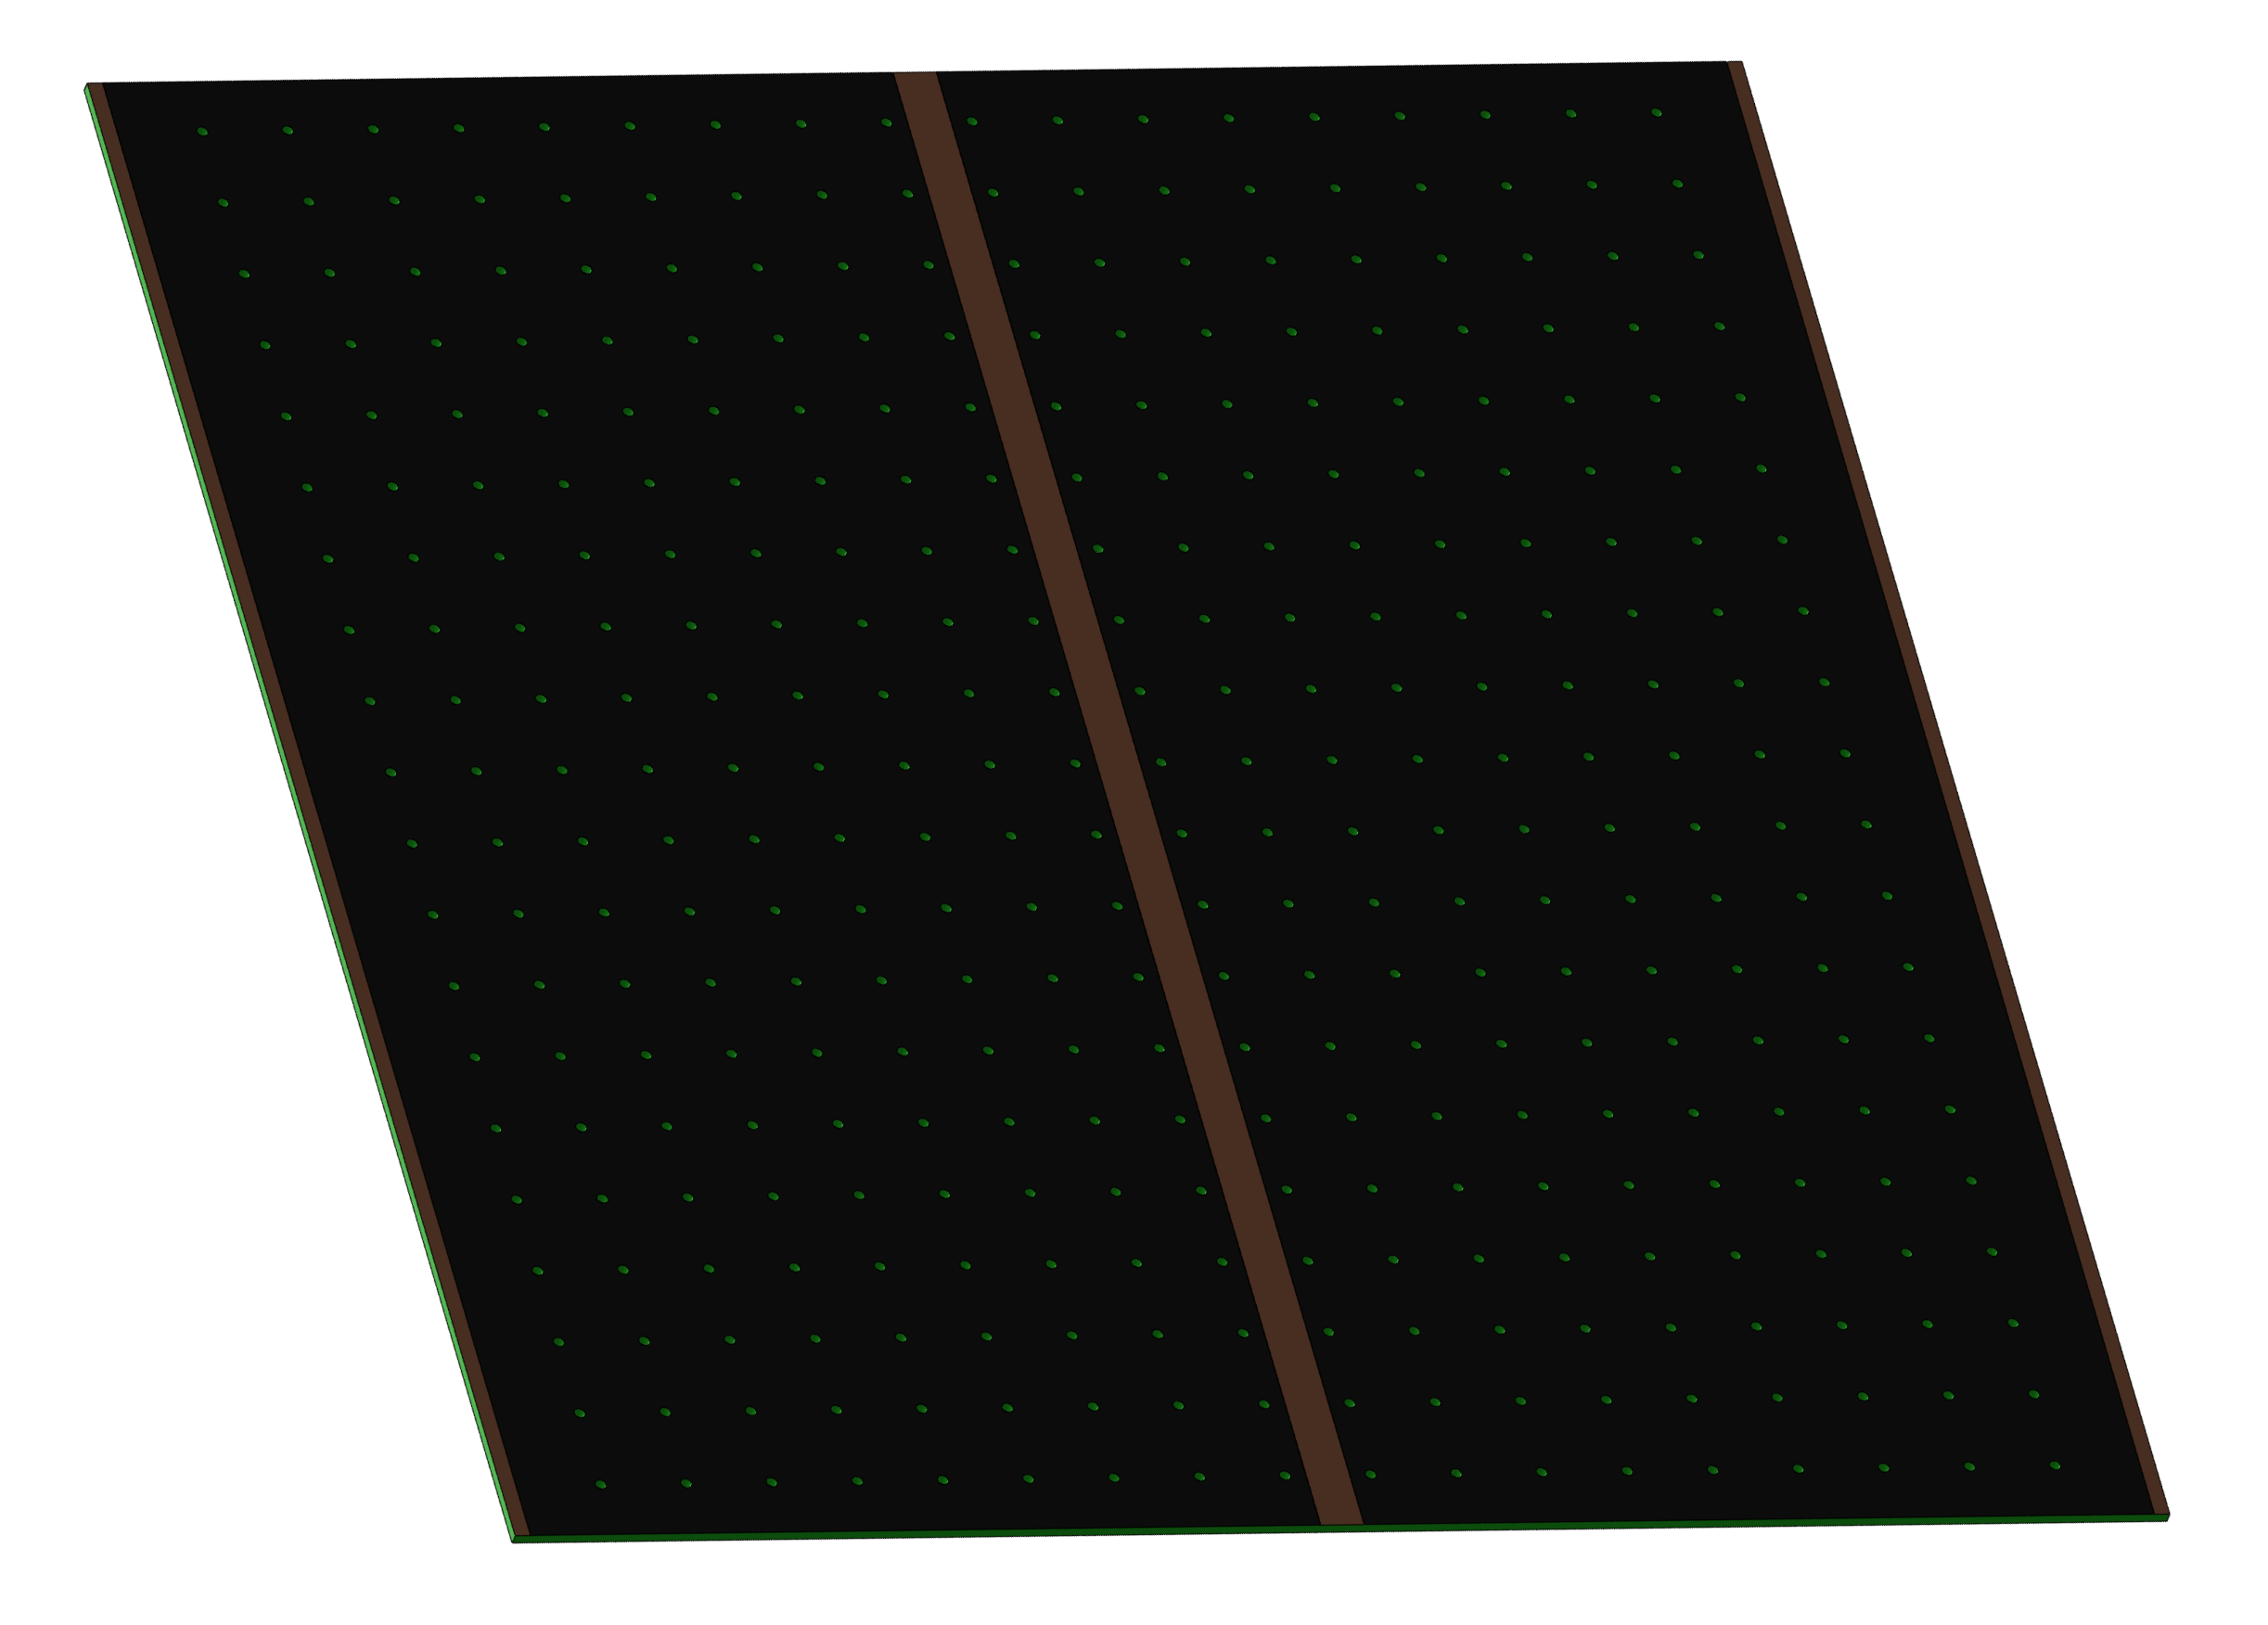
\includegraphics[width=\linewidth]{graphics/lartpc/FieldCage/fcbottomtop.PNG}
\end{minipage}
\caption{(Left) Exploded-view drawing of the field-shaping structure of a TPC module. (Top right) High-voltage socket at the top of the cathode. (Bottom right) Bottom field-shell panel.}
\label{fig:field_shell}
\end{figure}

The cathode panel is covered on both sides with a layer of 25\,$\mu$m-thick Kapton XC, a material which provides a $\mathcal{O}(1)\,$M$\Omega/\Box$ sheet resistance, identical to the one used in the protoDUNE-SP cathode~\cite{protodune-sp_tdr}. The use of a resistive material prevents damage to the TPC, including the electronics, in the event of a discharge. The conductivity of the cathode is selected to be sufficient to neutralize the positive argon ions at the same rate as they are collected by the cathode. The high voltage is fed to the cathode plate through a socket placed at the top of the panel. The high voltage is distributed to the field shell through a perimeter of copper cladding connected to the center copper strip of the four remaining panels by metalized G10 corner brackets bolted on with PEEK screws.

The field shell panels are covered with 100\,$\mu$m-thick sheets of Kapton DR8, a variant of Kapton XC which exhibits a higher $\mathcal{O}(1)\,$G$\Omega/\Box$ sheet resistance at room temperature and under low voltage loads. This material is a suitable basis to replace traditional field cages as it provides sufficient bulk resistance to constrain the heat load and limit the necessary power supply power. Kapton DR8 was extensively studied on $15\times15$\,cm$^2$ panels; figure~\ref{fig:dr8_studies} shows the apparatus used to conduct the tests and the sheet resistance of this material as a function of temperature and electric field, for various samples. These results show that at a peak electric field of 500V/cm and at liquid argon temperature, the sheet resistance of DR8 is $\sim3\,$G$\Omega/\Box$. Accounting for a shell aspect ratio of $L/W=1/16$ on either side of the cathode, the bulk resistance of a module is $R\simeq100$\,M$\Omega$. For a cathode voltage of $V=25$\,kV, this corresponds to a total heat load $V^2/R<10$\,W spread over the entire shell, or a local heat density of $<100\mu$W/cm$^2$, well below the maximum value.

\begin{figure}[htbp]
\centering
\begin{minipage}[b]{.295\textwidth}
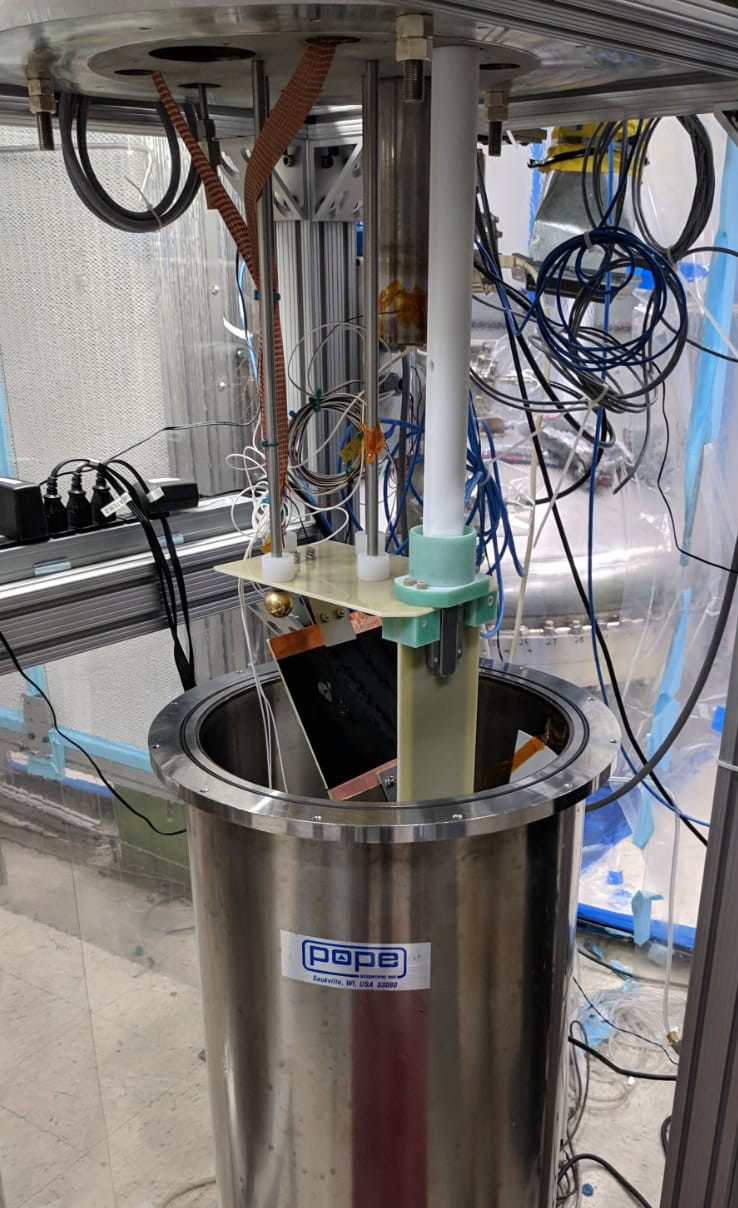
\includegraphics[width=\linewidth]{graphics/lartpc/FieldCage/ir2_2.jpeg}
\vspace{2mm}
\end{minipage}
\qquad
\begin{minipage}[b]{.4\textwidth}
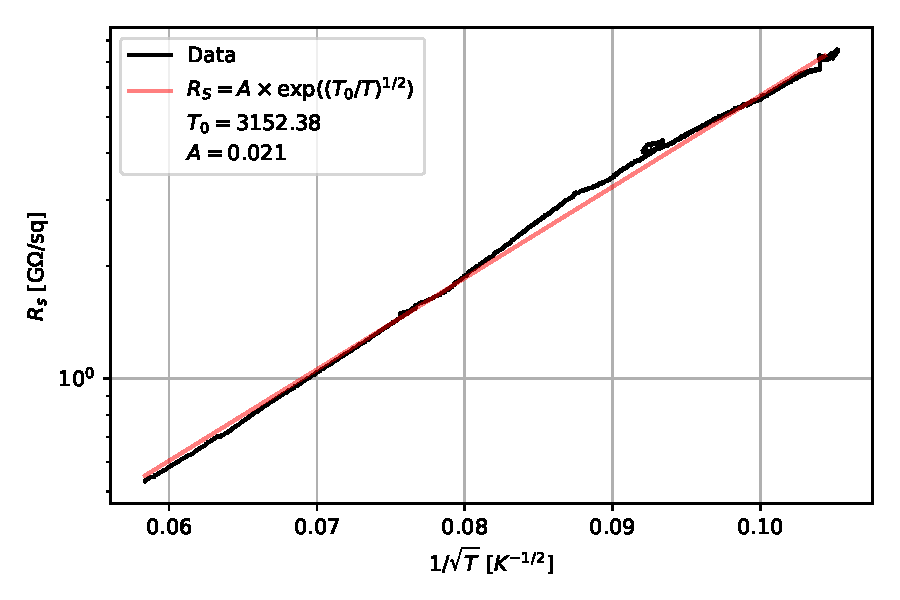
\includegraphics[width=\linewidth]{graphics/lartpc/FieldCage/ir2_temp_scan.pdf}
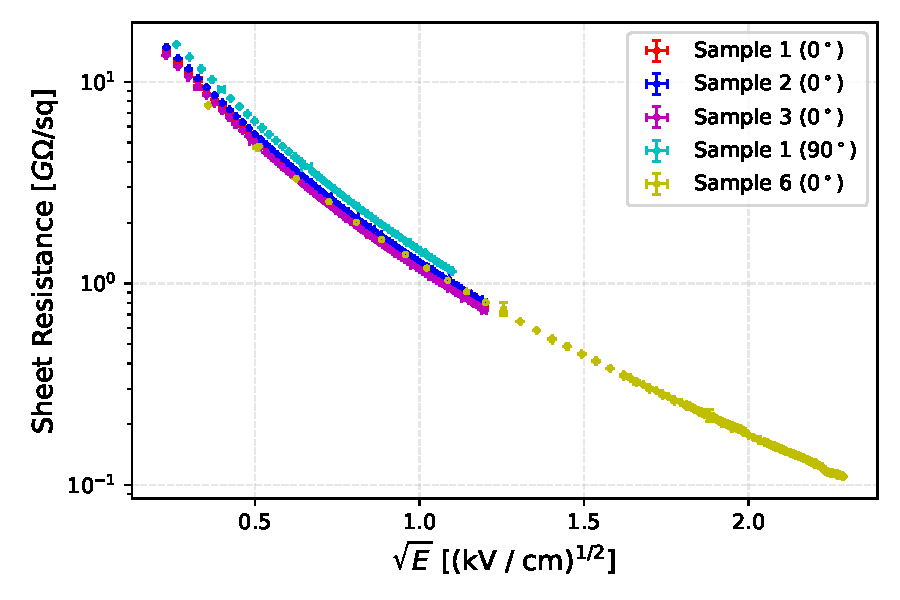
\includegraphics[width=\linewidth]{graphics/lartpc/FieldCage/ir2_efield.pdf}
\end{minipage}
\caption{(Left) Kapton DR8 test apparatus in a small-scale liquid-argon cryostat. (Right) Sheet resistance of DR8 at 125\,V/cm, as a function of temperature (top) and in liquid argon, as a function of electric field strength (bottom). Both graphs agree with the hopping transport model~\cite{hopping_transport}.}
\label{fig:dr8_studies}
\end{figure}

For the construction of a $2/3$-scale DUNE-ND prototype module, a method to laminate the conductive Kapton onto the copper-clad FR4 panels was demonstrated. It employed a purpose-built lamination device or `laminator' (left of figure~\ref{fig:field_shell_laminations}), and followed these steps:
\begin{enumerate}
    \item etch copper-clad FR4 panels to leave only a 1.25\,cm-thick bands of copper: around the perimeter for the cathode and in three separate strips for the field shell panels (one in the center to mate with the cathode and two on the sides to to connect to the anodes);
    \item laminate a sheet of protective plastic on the back of the panel, plug the the screw holes with rubber and mask part of the copper bands with tape to prevent epoxy from getting on them;
    \item tape Kapton sheets in the desired pattern onto the laminator table, laminate them with protective film, lift the film off the table;
    \item apply $250$\,g/m$^2$ of Master Bond EP29LPSP epoxy, roll two parallel DR8 sheets on either side of the central copper band, ensure $>5\,$mm overlap with each band;
    \item cover the laminate with bleeder cloth, vacuum bag the assembly, cure for seven days at room temperature, including two days under vacuum.
\end{enumerate}
A cathode and a side panel produced using this method are pictured in the center and on the right of figure~\ref{fig:field_shell_laminations}, respectively. Proper electrical contact of the Kapton XC to the perimeter of the cathode is tested by measuring the current from a surface probe to the perimeter. Similarly, contact between the Kapton DR8 and the copper bands is assessed by measuring the current flowing from the center copper strip to either side strips. In the prototype, current was measured in all field-shaping panels and will be further tested in a data acquisition run.

\begin{figure}[htbp]
\centering

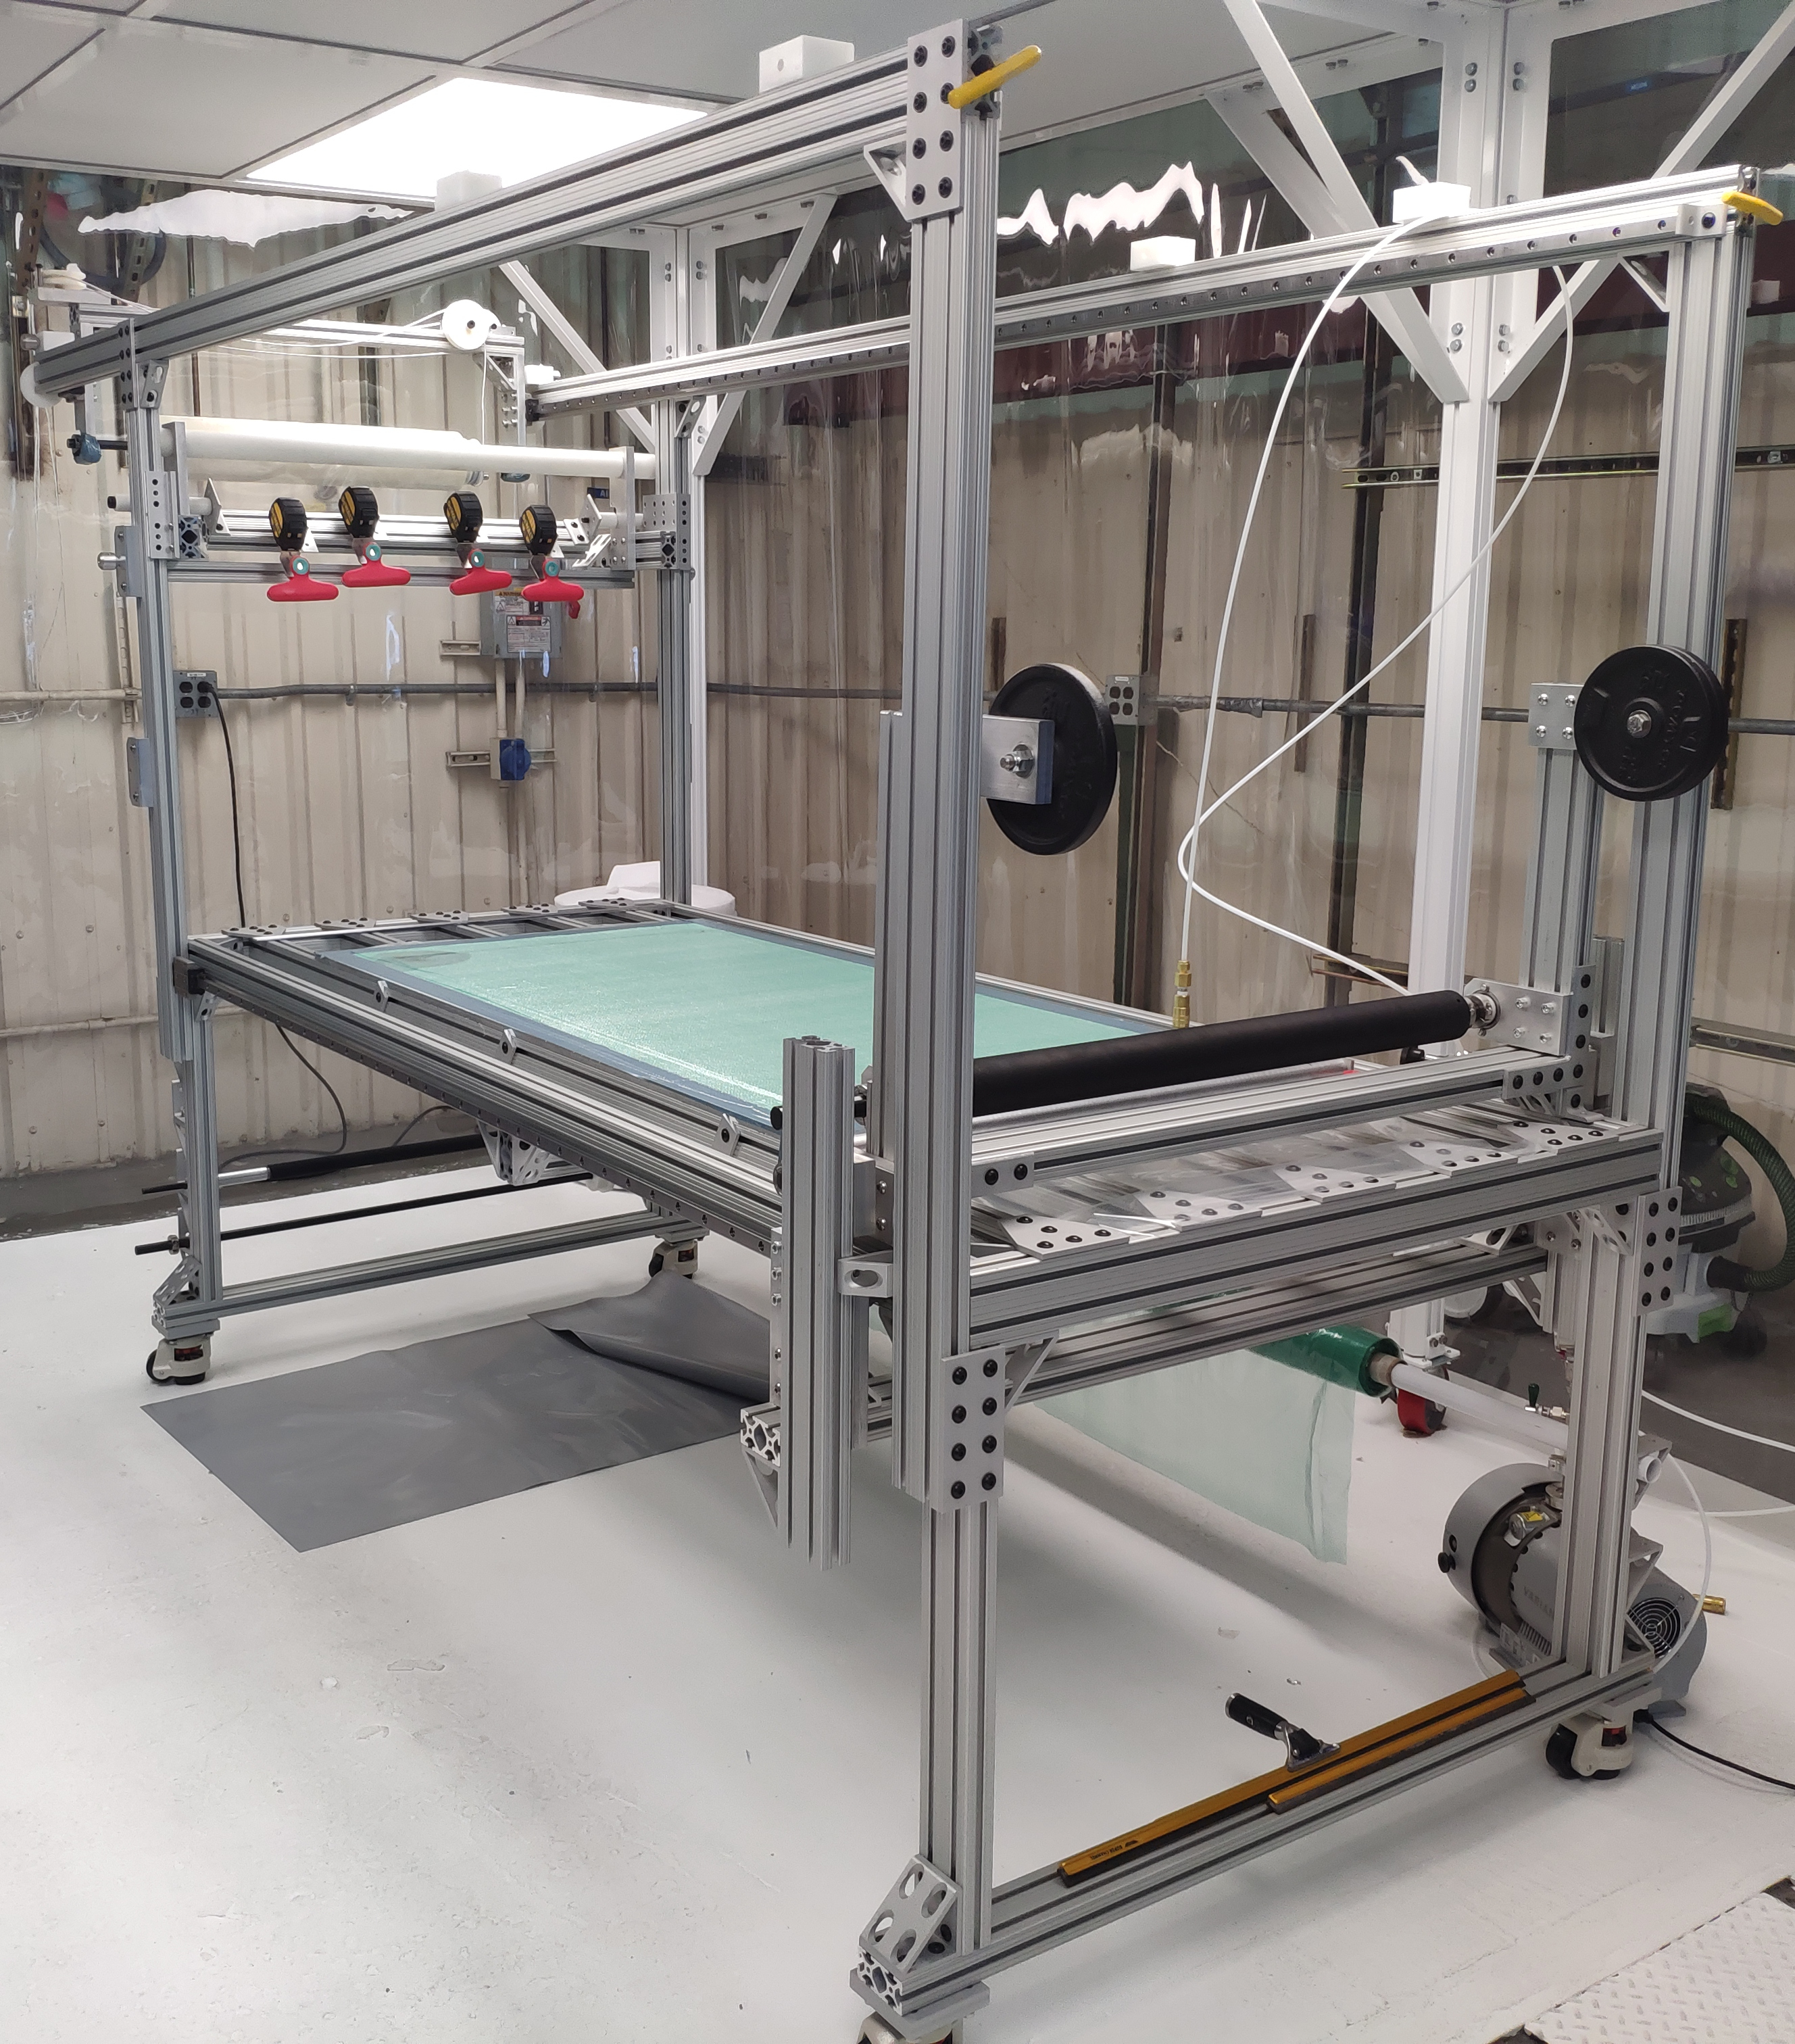
\includegraphics[width=.3\linewidth]{graphics/lartpc/FieldCage/laminator.jpg}
\qquad
\includegraphics[width=.25\linewidth]{graphics/lartpc/FieldCage/cathode_picture.jpg}
\qquad
\includegraphics[width=.25\linewidth]{graphics/lartpc/FieldCage/side_panel_picture.jpg}
\caption{(Left) Lamination device used to adhere Kapton onto FR4 panels. (Center) $2/3$-scale DUNE ND-LAr TPC cathode and (Right) field-shell side panel.}
\label{fig:field_shell_laminations}
\end{figure}


\subsection{Charge Readout}
\label{sec:lartpc-des-chargero}
{\it Brooke, 5 pages}
\subsubsection{Overview}
\label{sec:lartpc-cro-ovvw}
The charge readout system senses and records the signals of liquid argon ionization by charged particles traversing the LArTPC\@.
It must record signals with spatial granularity at the same level or better that the Far Detector in order to enable a high-fidelity prediction of the neutrino signal at the Far site.
The ND LArTPC relies on a novel pixelated anode with 4~mm pixel spacing and 2.5~$\mu$s signal time-binning in order to provide a true 3D record of the ionization signals.
This true 3D imaging is required to overcome signal pileup in the high-rate environment of the Near site, as discussed in Sec.~\ref{sec:ndlar-pileup}\@.

The core element of the charge readout system is the LArPix pixel anode tile, as shown in Fig.~\ref{fig:ndlar-pixeltile}.
These are printed circuit boards adapted to serve as self-triggering charge-sensitive anode surfaces within the ND LArTPC, and instrumented with the custom LArPix low-power cryogenic-compatible application-specific integrated circuit (ASIC)\@. 
A single 34-pin twisted-pair ribbon cable provides power and data for each tile.
These cables are connected to a custom PCB-based feed-through mounted on the cryostat lid, directly above each TPC module.
Four PACMAN controllers are mounted in metal enclosures attached to the outside surface of each module feed-through, providing filtered power and noise-isolated data input-output to the tiles.
These controllers in turn receive an external 10~MHz clock and/or sync signal for data synchronization, as well as optional external triggers signals from the light readout system.
A Weiner PL506 24~V power supply delivers power to 20 controllers.
Standard RJ-45 ethernet cables carry data to and from the controllers, and are aggregated in a rack-mounted ethernet switch.
An optical fiber connection transmits data to and from this switch to the Near site DAQ system.
Fig.~\ref{fig:larpix-architecture} outlines the charge readout system architecture, and Tab.~\ref{tab:ndlar-chargescope} outlines the institutional responsibilities.

% ND-LAr Pixel Anode Tile
\begin{dunefigure}[LArPix Tile]{fig:ndlar-pixeltile}
{The LArPix pixel anode tile with 10,240 self-triggering charge-sensitive pixels.  Each TPC anode is composed of 20 identical tiles arranged in two columns.}
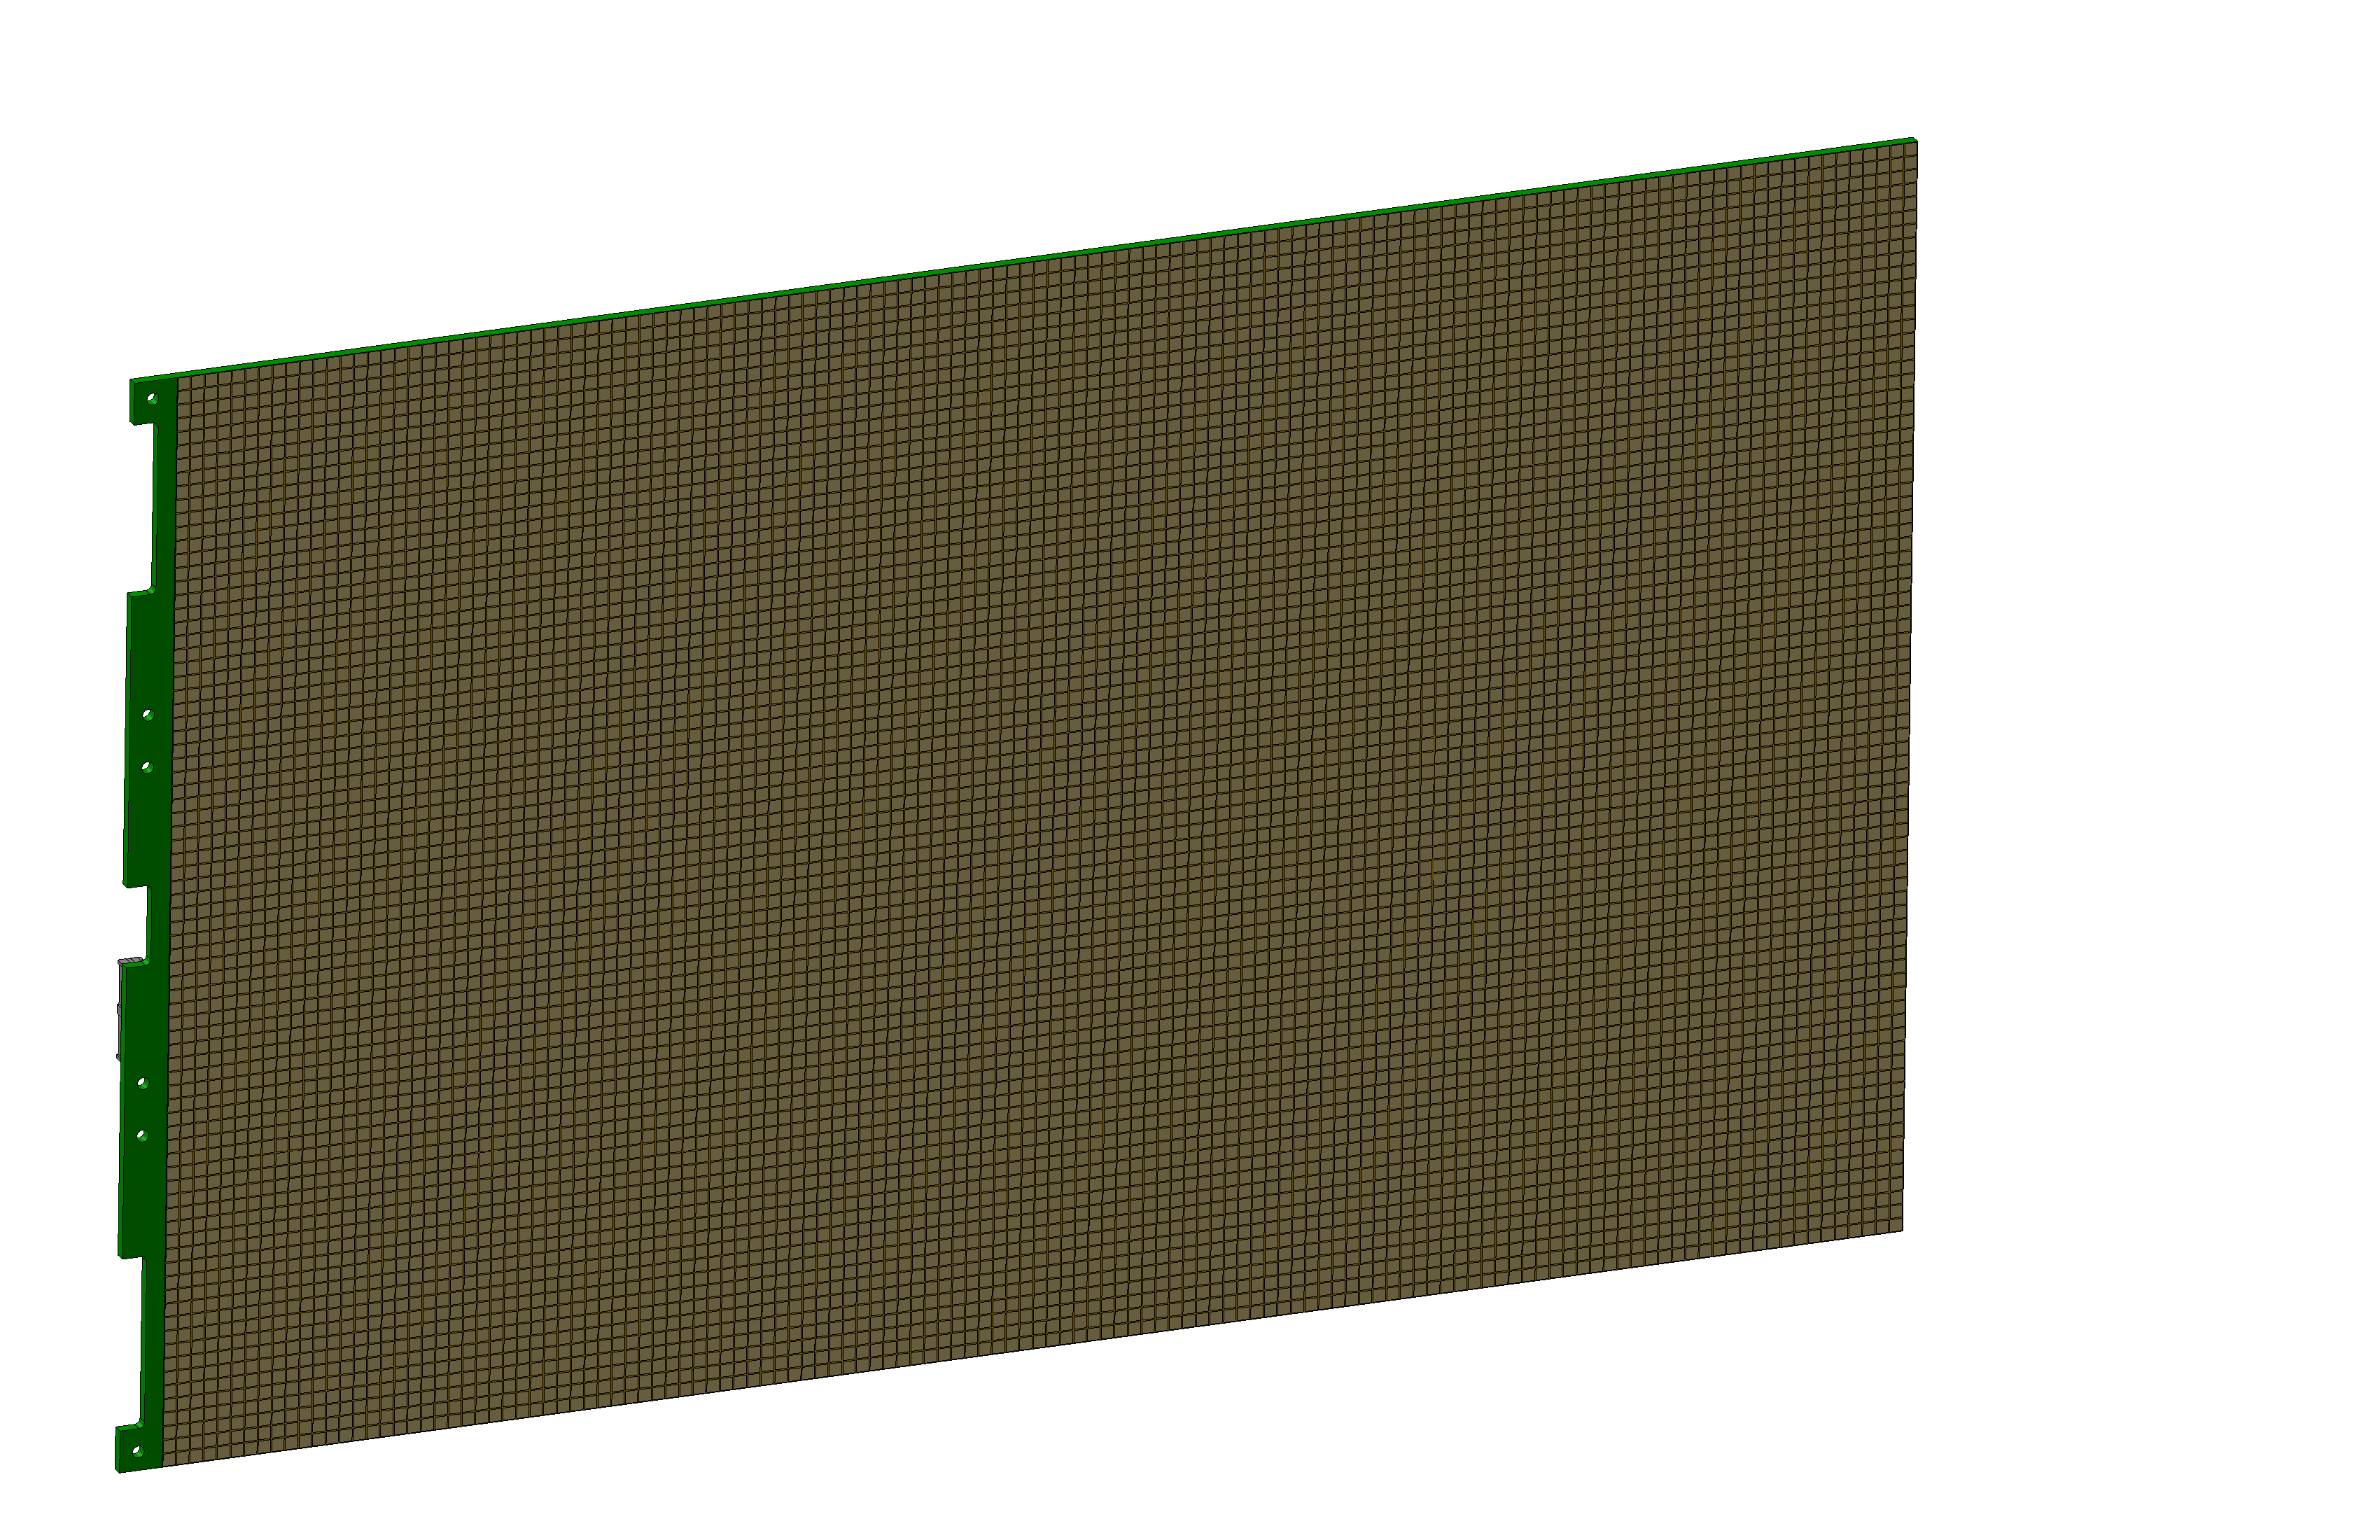
\includegraphics[width=0.8\textwidth]{graphics/lartpc/Charge/larpixiso.PNG}
\end{dunefigure}

% LArPix System Architecture
\begin{dunefigure}[LArPix Architecture]{fig:larpix-architecture}
{The LArPix system architecture for the ND-LAr detector.}
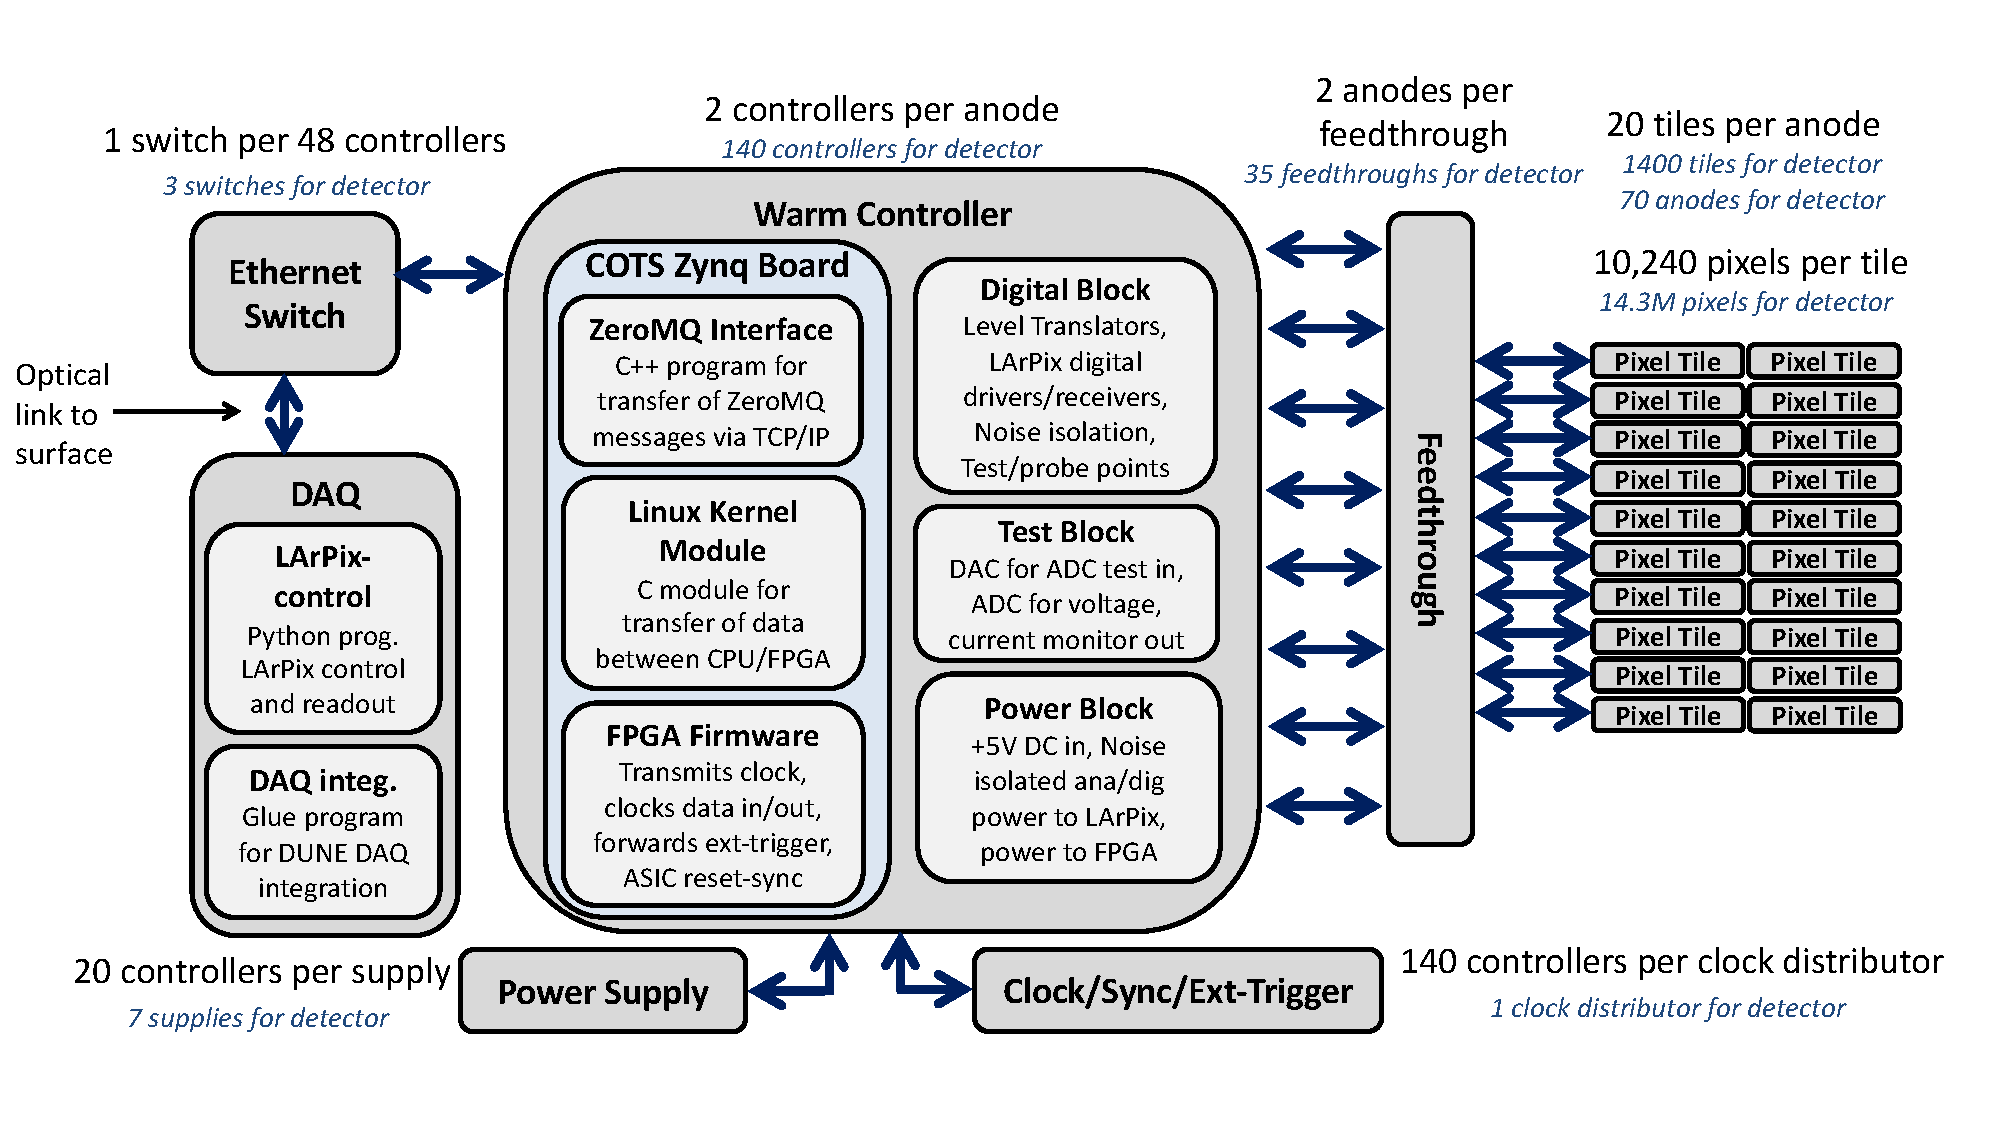
\includegraphics[width=0.8\textwidth]{graphics/lartpc/Charge/LArPix_NDArchitecture_12Nov2020.pdf}
\end{dunefigure}

% Charge Readout Partners
\begin{dunetable}
[ND-LAr Charge Readout Institutions]
{ll}
{tab:ndlar-chargescope}
{Institutional responsibilities in the ND-LAr charge readout system.}
Task & Institutions \\ \toprowrule
ASIC design and production & LBNL \\ \colhline
ASIC test boards & UPenn \\ \colhline
ASIC testing & Caltech, UCSB \\ \colhline
Tile design and production & LBNL \\ \colhline
Tile testing & UTA \\ \colhline
Cables and Feed-throughs & Rutgers \\ \colhline
PACMAN hardware & UC-Davis \\ \colhline
PACMAN firmware & UC-Irvine \\ \colhline
Clock and Power & LBNL \\ \colhline
DAQ interface software & LBNL \\ % no \colhline on final row
\end{dunetable}
\subsubsection{Charge Readout Key Requirements}
\label{sec:lartpc-cro-req}
The key driving design requirements and performance requirements for the field structure are summarized in Figures~\ref{fig:lartpccroreq1},~and \ref{fig:lartpccroreq2}. 

\begin{figure}
\centering 
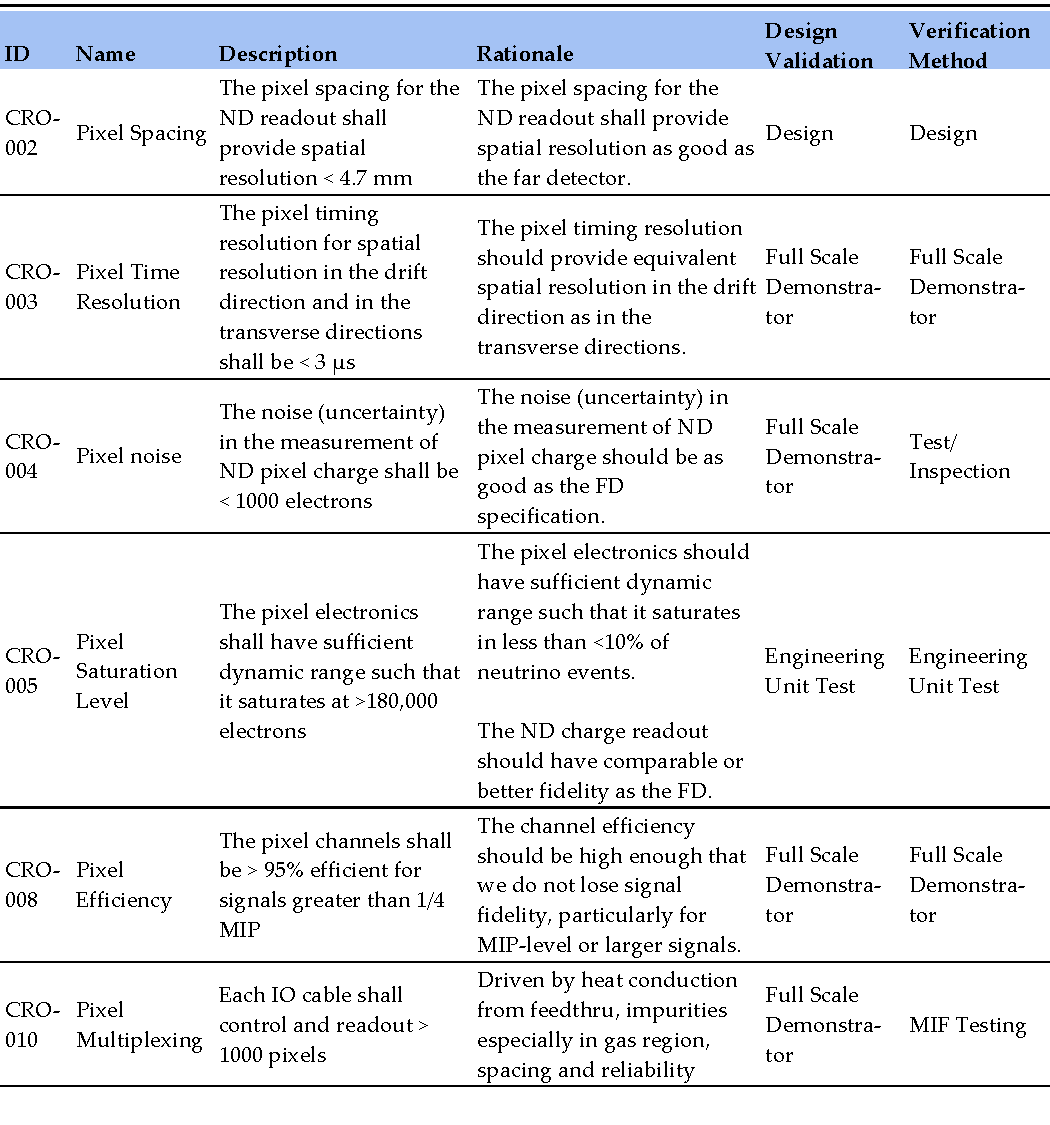
\includegraphics[width=1\linewidth]{graphics/lartpc/0Req/NDCROreqs1.pdf}
\caption{\label{fig:lartpccroreq1} ND LArTPC Key Charge Readout Requirements (1)}
\end{figure}
\begin{figure}
\centering 
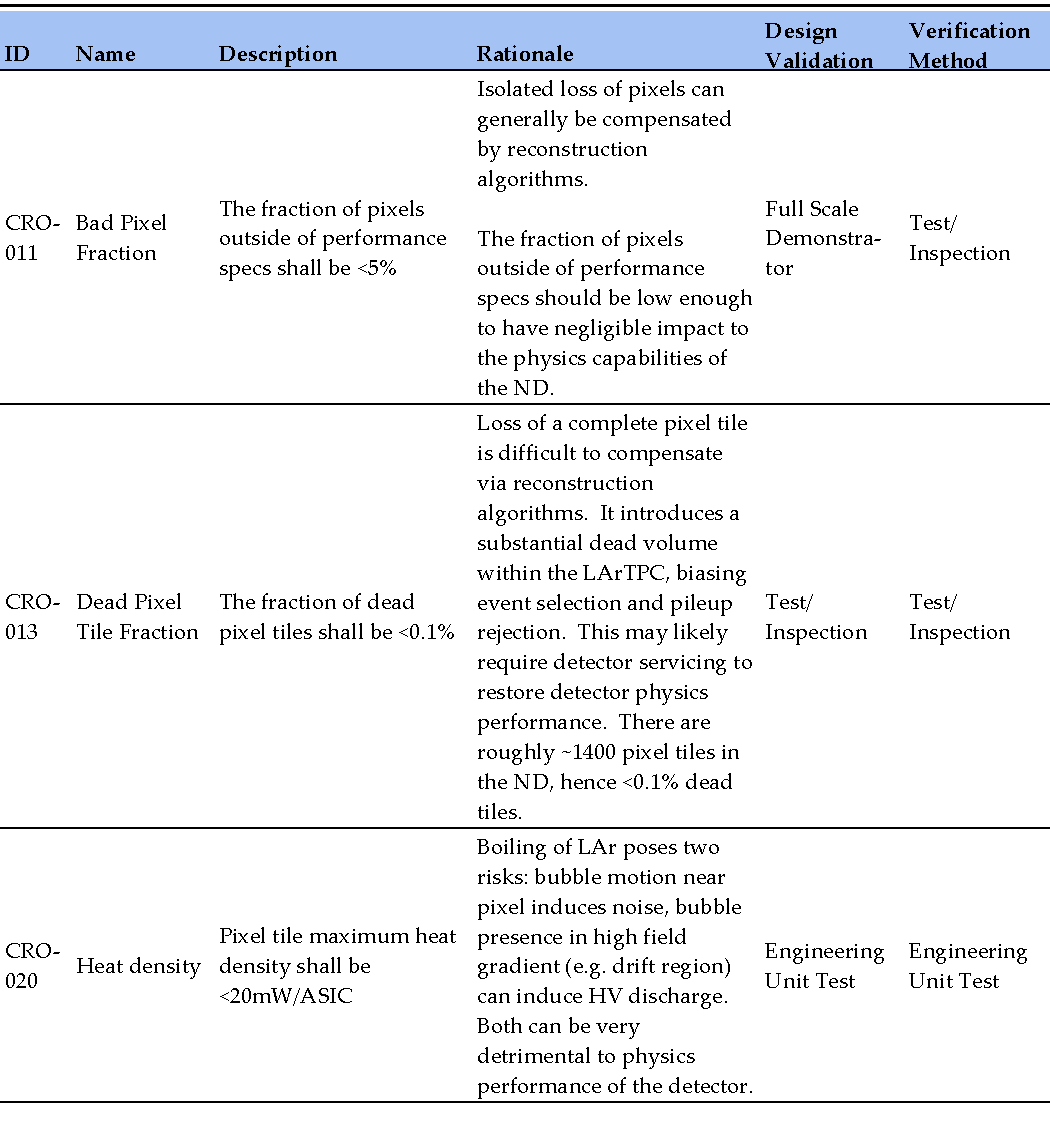
\includegraphics[width=1\linewidth]{graphics/lartpc/0Req/NDCROreqs2.pdf}
\caption{\label{fig:lartpccroreq2} ND LArTPC Key Charge Readout Requirements (2)}
\end{figure}


The charge readout system design is driven by requirements that fall in three categories: performance, manufacturability, and reliability.
For performance, the charge readout system must deliver 3D spatial granularity at least as good as the Far Detectors.
This drives the pixel spacing of $<$4~mm, and a corresponding density of $>$60,000 channels per square meter.
A noise level of $<$1000~e$^-$~ENC and dynamic range of $>$200,000~e$^-$ matches the Far Detector requirements on signal fidelity.
With a measured heat production of roughly 100~$\mu$W per channel, the tile heat density is below the threshold where detrimental boiling of the liquid argon occurs.

The ND LArTPC requires more than 200~m$^2$ of pixel anode, motivating requirements that facilitate large-scale production and control.
The pixel tile is designed so that it relies on standard multi-layer printed circuit board layout and production techniques, allowing it to be produced and assembled by typical PCB vendors.
Each LArPix ASIC instruments 64 pixels, enabling tiling of ASICs and pixel at the targeted 4~mm pitch without resorting to novel assembly techniques.
The ASICs are packaged to enable assembly via standard pick-and-place and solder re-flow techniques, as well as leveraging vendor-based post-assembly quality control inspection.
Control and readout of approximately 5,000 pixels within a pixel tile has been demonstrated over one I/O channel (four conductors operating at 10~MHz), achieving the high channel density required for the detector with a viable number of cables and feed-throughs.

Given the difficulty to access the detector once the cryostat is filled with liquid argon, the design of the cold-side components must be reliable.
The loss of a few percent of pixels, either individually or for an entire 64-pixel ASIC, does not considerably impact detector performance.
On the other hand, loss of an entire pixel tile would substantially hinder event reconstruction, efficient pileup rejection, as well as accurate event fiducialization.
(To understand this, consider the ease of interpolating the signal for a missing 4~mm-by-4~mm pixel or 3~cm-by-3~cm ASIC anode region against the relative difficulty of guessing an unknown signal within the 30~cm by 50~cm region of an entire tile.) 
For this reason, the pixel tile and it's associated cable and feed-through connections must be very reliable.
Reliability is achieved by minimizing the number of unique parts and the number of active elements.
The tile is also designed to be robust to failure of individual ASICs, and each tile has 4 redundant data I/O connections to the warm-side PACMAN controller. 
These aspects of the system design will be described in detail later in this section.

\subsubsection{LArPix ASIC}
\label{sec:larpix-asic}

The LArPix ASIC is a custom low-power cryogenic-compatible integrated circuit that enables true 3D charge readout of LArTPCs\@.
It is a mixed-signal chip, consisting of 64 analog front-ends amplifiers, 64 analog-to-digital converters, and a shared digital core than manages chip configuration and data I/O\@.
The challenge for this ASIC design is to meet the requirements in detector granularity and low-noise performance at sufficiently low-power so as not to boil the detector.
The initial LArPix-v1 prototype demonstrated the viability of pixelated readout, achieving $<$300~e-~ENC in liquid argon at a average power of 62~$\mu$W per channel\fixme{add citation here}.
The LArPix-v2 ASIC added many improvements to facilitate it's use with large-scale pixel anodes, as discussed later in this section.

To meet the stringent power requirements, the LArPix ASIC exploits the sparse nature of ionization signals in LArTPCs\@.
Although these detectors are highly-granular, ionization signals generally occupy only a very small fraction of the total TPC volume.
LArPix is designed to avoid digitation and readout of this mostly quiescent data.
Fig.~\ref{fig:larpix-design} shows a conceptual diagram of the LArPix design.
Each pixel channel functions as an independent self-triggered detector.
As an ionization signal is collected on a pixel, it is amplified by a charge-sensitive amplifier (CSA)\@.
The amplifier is operated in an integrating mode with no resistive feedback, therefore the amplifier output grows monotonically at roughly 1~mV per 250~electrons received at the input.
A buffer drives this signal to a discriminator that can be tuned uniquely for each channel.
When the buffer output exceeds the discriminator threshold, a hit signal is issued to the digital control and a timestamp counter (100~ns precision) is latched.
After a tunable delay, generally set at 1.8~$\mu$s to allow full collection of ionization signals of a few-mm extent in the drift direction, the ADC samples and digitizes the signal as a single 8-bit digital charge value.
The charge ADC and timestamp are then formatted into an output hit record, including the channel ID and chip ID to uniquely identify the pixel, and passed to {\em serial out} for transmission out of the detector.
Simultaneously to the ADC sampling the signal, the CSA is reset.
This discards the charge present at its input, refreshing it to receive subsequent signals.
The minimum time between two hit records on a channel depends on the tunable delay discussed above, but is typically 2.6~$\mu$s, providing a granularity of 4~mm in the drift direction assuming a drift velocity of 1.6~$\mu$s at a drift field of 500~V/cm\@.
Therefore, each pixel tile can be thought of as an aggregation of thousands of independent charge detectors each with 100\% uptime.
In practice each channel is also periodically reset at a tunable frequency (typically 10~Hz to 100~Hz) in order to discard spurious charge that collects on the input. This spurious charge is primarily due to charge leakage present within the ASIC itself, measured to be approximately 500~e$^-$/s at liquid argon temperatures.

\begin{dunefigure}[LArPix ASIC Design]{fig:larpix-design}
{A conceptual diagram of a single low-power LArPix ASIC front-end channel.}
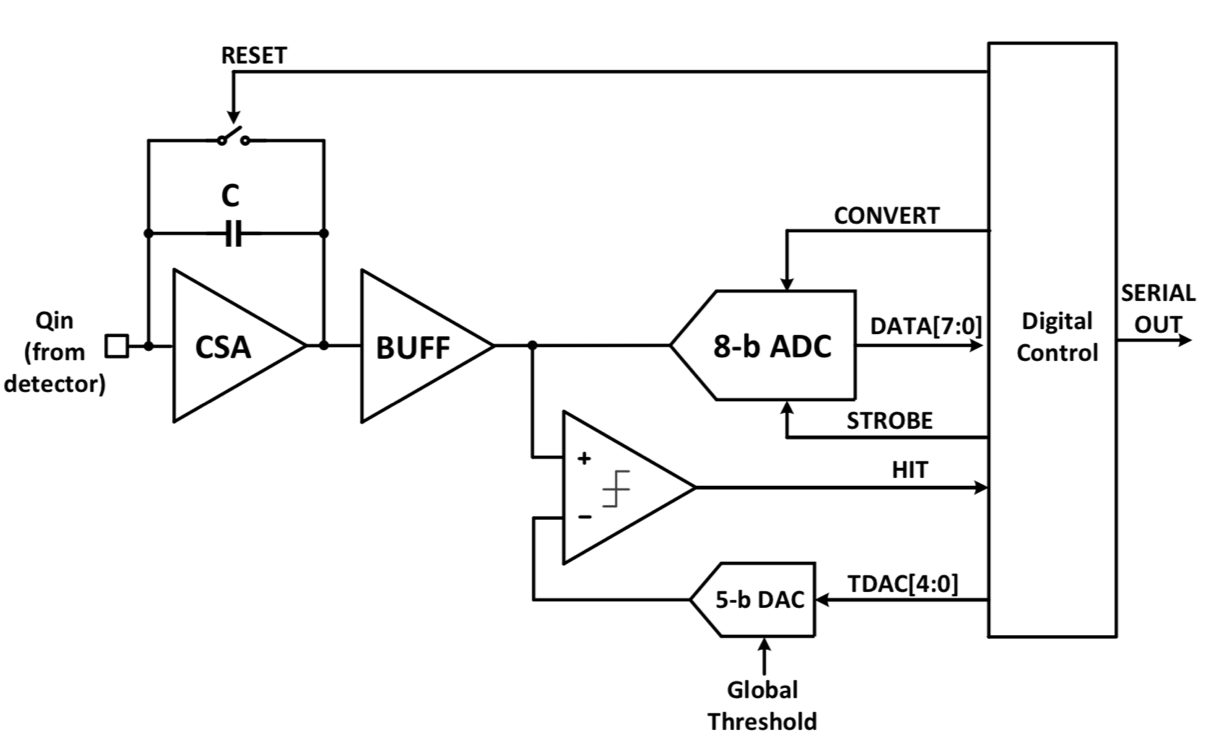
\includegraphics[width=0.8\textwidth]{graphics/lartpc/Charge/larpix_frontend.png}
\end{dunefigure}

The power used for data I/O increases with transmission speed.
To manage this power, the hit records are buffered within on-chip SRAM memory and then slowly transmitted out serially at a tunable rate (5~Mb/s default)\@.
The memory is structured as a single large internal FIFO of length of 2096 records, providing sufficient capacity to capture bursts of incoming hit data and then slowly transmitting them out of the detector at minimal power.
Each hit record contains two bits to mark the FIFO status (half-full or full) at the time of hit record production, as well as a parity bit for checking data integrity.

Photographs of the LArPix-v1 and v2 bare dies are shown in Fig.~\ref{fig:larpix-dies}.
LArPix-v1 was developed as a proof-of-concept for pixel LArTPC readout, while the main goal LArPix-v2 was to facilitate scalable commercial production of pixel anode tiles.
This second-generation chip has 64 input channels per chip, twice that of v1\@.

The original 6-bit ADC was converted to 8-bit\@.

\begin{dunefigure}[LArPix ASIC Bare Dies]{fig:larpix-dies}
{(Left) The prototype LArPix-v1 ASIC, with 32 input channels arranged in two columns around a digital core.  (Right) The LArPix-v2 ASIC, with 64 input channels arranged along the four edges around a digital core containing four SRAM memory blocks.}
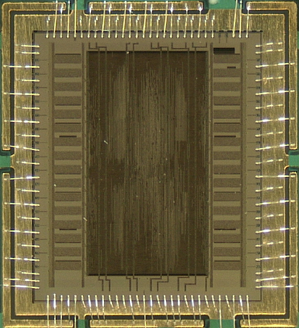
\includegraphics[width=0.35\textwidth]{graphics/lartpc/Charge/larpix_v1_die.png}
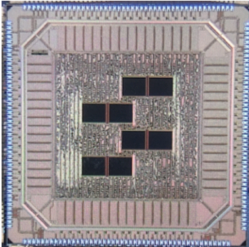
\includegraphics[width=0.4\textwidth]{graphics/lartpc/Charge/larpix_v2_die.png}
\end{dunefigure}

% Hydra I/O


\subsubsection{LArPix Anode Tile}
\label{sec:larpix-tile}

Each tile 
Each TPC module anode consists of 20 identical pixel tiles, arranged in two columns.
The inner-facing surface is covered by charge-sensitive pixels, or more accurately gold-coated conductive pads, at a pitch of 4~mm\@.


% Prototype Pixel Anode Tile
\begin{dunefigure}[LArPix Prototype PixelTile]{fig:prototype-pixeltile}
{}
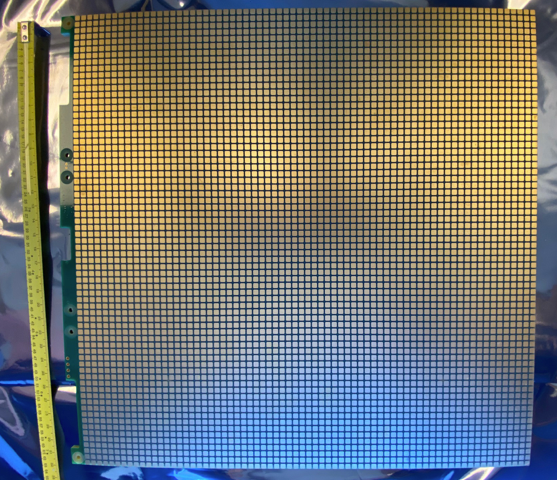
\includegraphics[width=0.4\textwidth]{graphics/lartpc/Charge/larpix_v2_10x10tile_frontside.png}
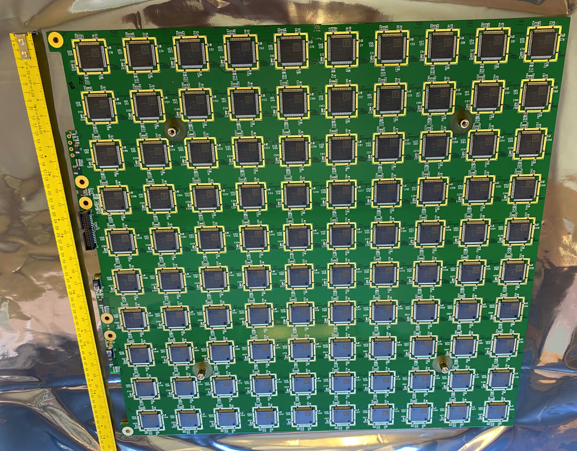
\includegraphics[width=0.43\textwidth]{graphics/lartpc/Charge/larpix_v2_10x10tile_backside.png}
\end{dunefigure}



\subsubsection{Cables and Feed-throughs}
\label{sec:larpix-feedthroughs}

\subsubsection{PACMAN Controller}
\label{sec:larpix-control}

\subsubsection{Clock, Data, and Power}
\label{sec:larpix-clockdatapower}




%\begin{itemize}
%    \item Intro 
%    \begin{itemize}
%        \item Purpose of subsystem
%        \item Key elements of subsystem
%        \item Major requirements that drive subsystem design
%    \end{itemize}
%    \item Subsystem details
%    \begin{itemize}
%        \item Component descriptions, counts per module/detector
%        \item Figure: CAD of subsystem elements
%        \item Subsystem interfaces (mechanical, electrical)
%        \item Component specifications
%        \item Component production process
%        \item Prototyping results / spec validation
%%    \end{itemize}
%\end{itemize}


\subsection{Light Readout}
%Authors N. Anfimov, A. Selyunin
%req ~ 5 pages.
\label{sec:lartpc-des-lightro}

\subsubsection{Overview}
The Light Readout System (LRS) provides fast timing information from the prompt scintillation light emitted by the charged particles in LAr at $\sim$\SI{128}{\nano\metre} wavelengths along with ionization. The optical detection of scintillation photons provides both an absolute reference ($t_0$) and rejection of unassociated charge signals (pileup) from the specific neutrino signals of interest. Furthermore, the LRS serve as a new dielectric light detection technique capable of being placed inside the field-shaping structure to increase light yield and localization of light signals.

The Light Readout System consist of two functionally identical, SiPM-based systems for efficient detecting single UV photons with a large surface coverage: the Light Collection Module (LCM) and the ArCLight module (ArCLight). readout, front-end electronics, DAQ (ADCs, synchronization and trigger), feedthrough flanges, SiPMs power supply subsystem, and slow control are also included in the system. Cabling and interconnection between elements are also provided by the system.

Each detector module (\num{35} in total) contains of \num{60} LCM and \num{20} ArCLight modules with the alternating arrangement (\num{3} LCM - \num{1} ArCLight). Surface coverage is shared equally between both detectors. Each light module is read out by SiPMs which are located by pairs on a Printed Circuit Board (SiPM-PCB). Each LCM is read out by a single SiPM-PCB, but an ArCLight is read out by \num{3} SiPM-PCB boards. Three SiPM-PCBs are grouped together by insertion to a single E-shaped PCB - E-PCB. The E-PCB is intended to interface SiPMs signals to long micro-coaxial cable lines ($\sim2$m) which are connected to the feedthrough. A transferring of small single photo-electron signals (SiPM calibration) into a long cable line requires equipment of each E-PCB with \num{6} pre-amplifiers. In total, all light modules in a single TPC-module are driven by  \num{40} E-PCBs. Feedthrough PCB with microcoaxial cable connectors provides interconnection between cold and warm sides of the detector module. On the warm side at the top of the cryostat nearby the feedtrough flange output, a VME 6U crate is located. There are 35 crates in total that are placed on top support of the ND-LAr. Forty Microcoaxial cable assemblies routing SiPMs signals and deliver power for SiPMs and pre-amplifiers interconnecting a feedthrough with accosiated  VME crate. The crate contains front-end electronics boards in VME 6U standard: SiPM power supply PCB modules based on DACs (SiPM PCB), PCB modules with variable gain amplifiers (VGA PCB), control module PCB, and a Patch board that  groups signals and power together into a single cable assembly. Optionally, a trigger module will be placed into the crate to provide the trigger logic that drives the ADCs. All these modules are custom made. Signals from VGAs comes to the ADCs by means of twisted pair ribbon cables. Network switch provides optical connection between the ADCs and the DAQ computers. Rack with ADCs, optical switches, and HV source are located at some distance from the cryostat.  
All ADCs will be synchronized by means of White Rabbit (WR) protocol that guarantees subnanosecond precision of clock distribution. Charge clock will be synchronized with WR 10 MHz clock.Absolute WR timestamp is 8 ns that is enough to improve matching of light-to-charge events.
\subsubsection{Light Readout Key Requirements}
\label{sec:lartpc-lro-req}
The key driving design requirements and performance requirements for the field structure are summarized in Figures~\ref{fig:lartpclroreq1},~and \ref{fig:lartpclroreq2}. 

\begin{figure}
\centering 
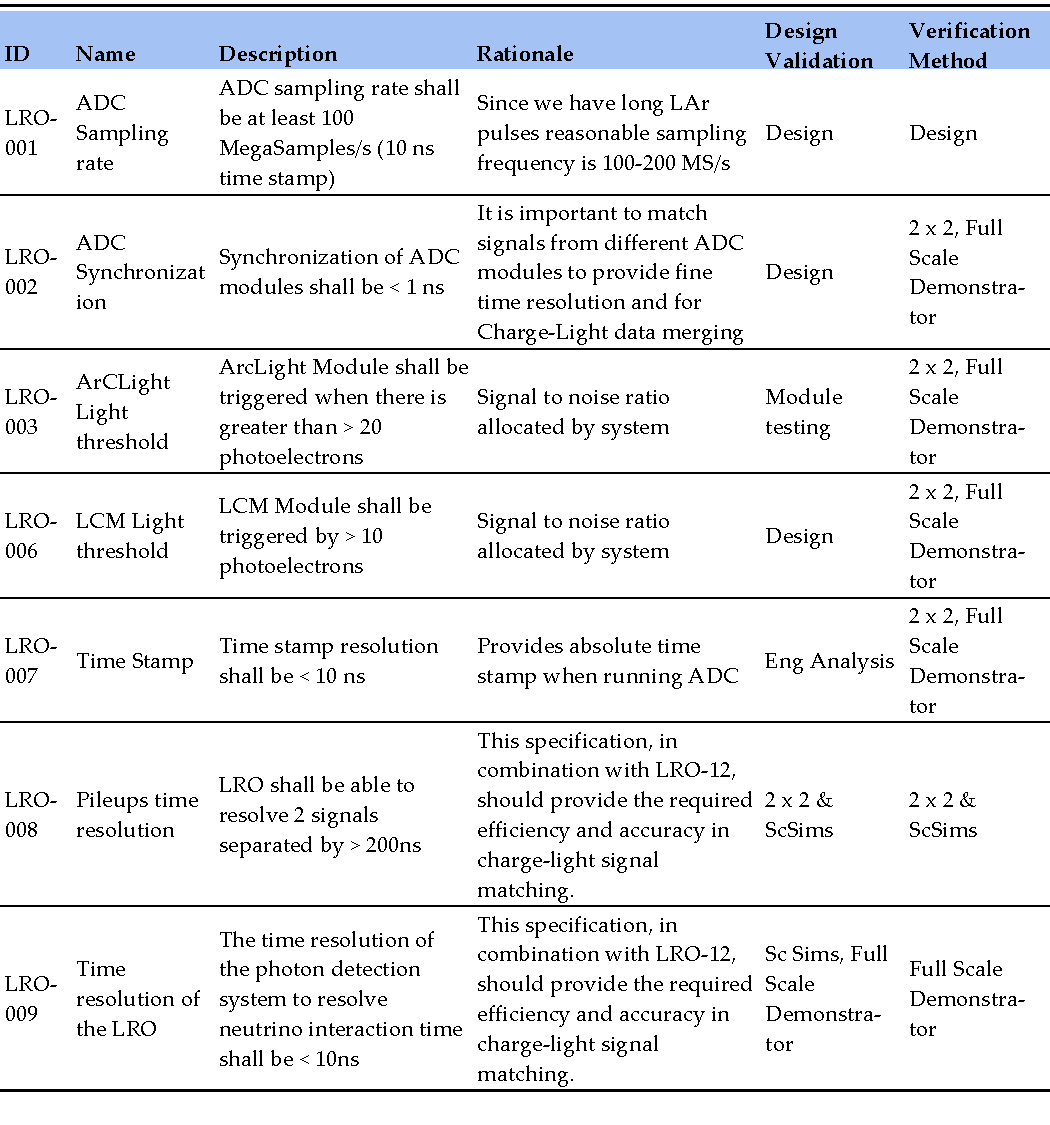
\includegraphics[width=1\linewidth]{graphics/lartpc/0Req/NDLROreqs1.pdf}
\caption{\label{fig:lartpclroreq1} ND LArTPC Key Light Readout Requirements (1)}
\end{figure}

\begin{figure}
\centering 
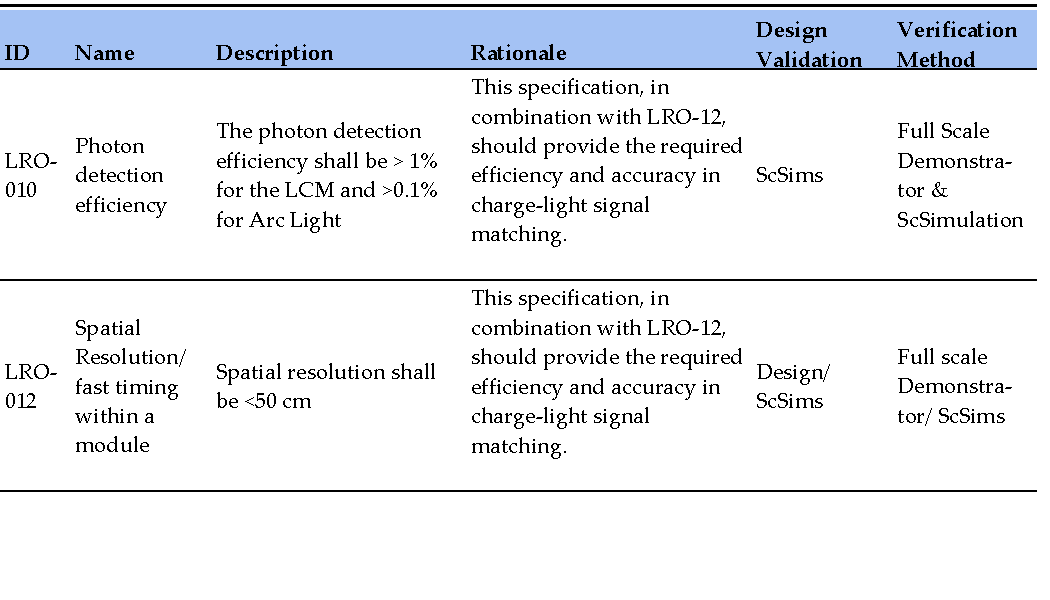
\includegraphics[width=1\linewidth]{graphics/lartpc/0Req/NDLROreqs2.pdf}
\caption{\label{fig:lartpclroreq2} ND LArTPC Key Light Readout Requirements (2)}
\end{figure}

\subsubsection{Physical operation principle}

An LCM and an ArCLight are share the same basic principle. The scintillation vacuum ultraviolet (VUV) light produced by LAr is shifted from \SI{128}{\nano\metre} to visible light by WaveLength Shiter (WLS), e.g. TPB - an efficient WLS, which is coated on the surface of the light collection systems. The emission spectrum of TPB is quite broad with a peak intensity of around \SI{425}{\nano\metre} (violet light). The violet light emitted on the surface of the light detection system eventually enters the bulk structure of the detector and is shifted to green light by a dopant (e.g. coumarin) in a bulk material which also acts as a light trap (see Fig.~\ref{fig:fig_modules}).
The ArCLight module (Fig.~\ref{fig:fig_modules}~left) has been developed by Bern University uses the ARAPUCA principle of the light trapping. The general idea is to let the violet light go into the shifter bulk to be re-emitted and produce a reflective coating for the green light on all sides but the photosensor window. On the TPB side a dichroic filter which is transparent for the violet light and reflective for the green is used. All other sides are coated with  mirror film or layer. The green light, hence, is trapped and may be detected by Silicon Photomultipliers (SiPMs). The ArcLight dimensions are \SI[product-units=repeat]{300x\sim500x10}{\milli\metre}.

\begin{figure}[htbp]
\centering 
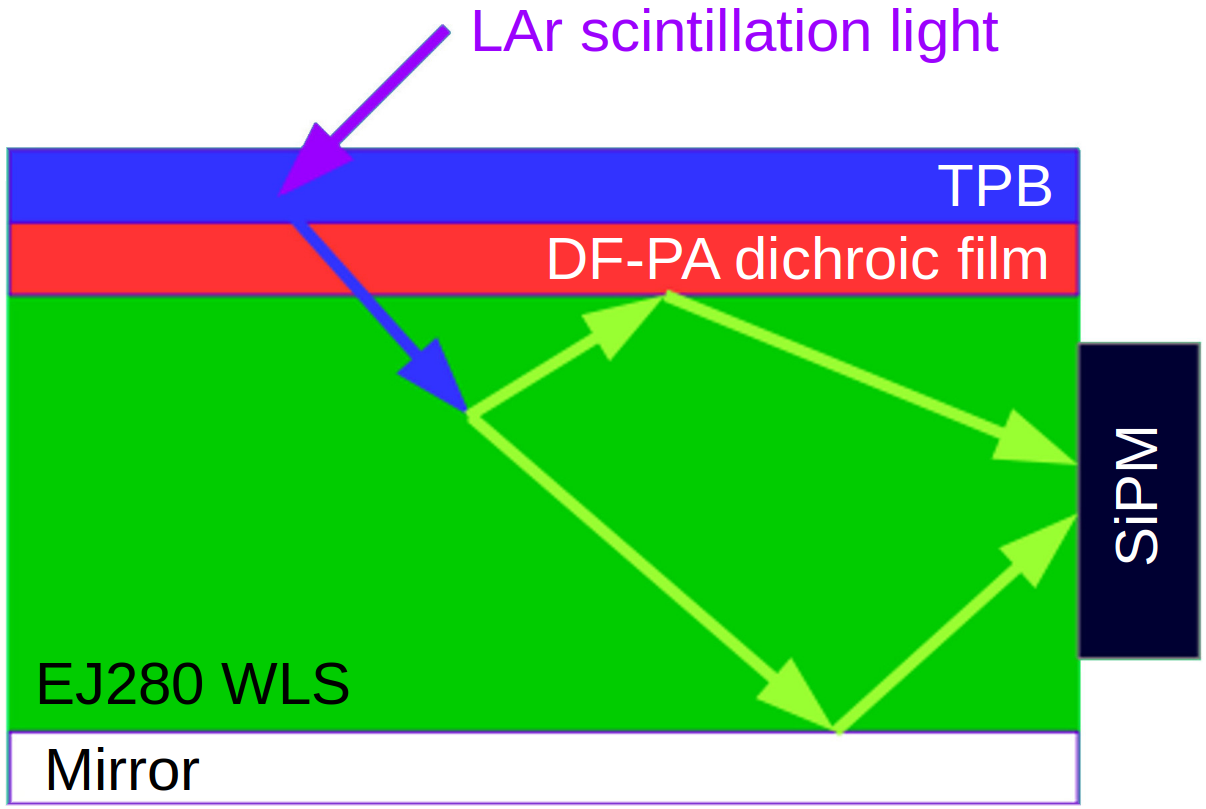
\includegraphics[width=0.44\linewidth]{graphics/lartpc/Light/ArCLight.png}
\qquad
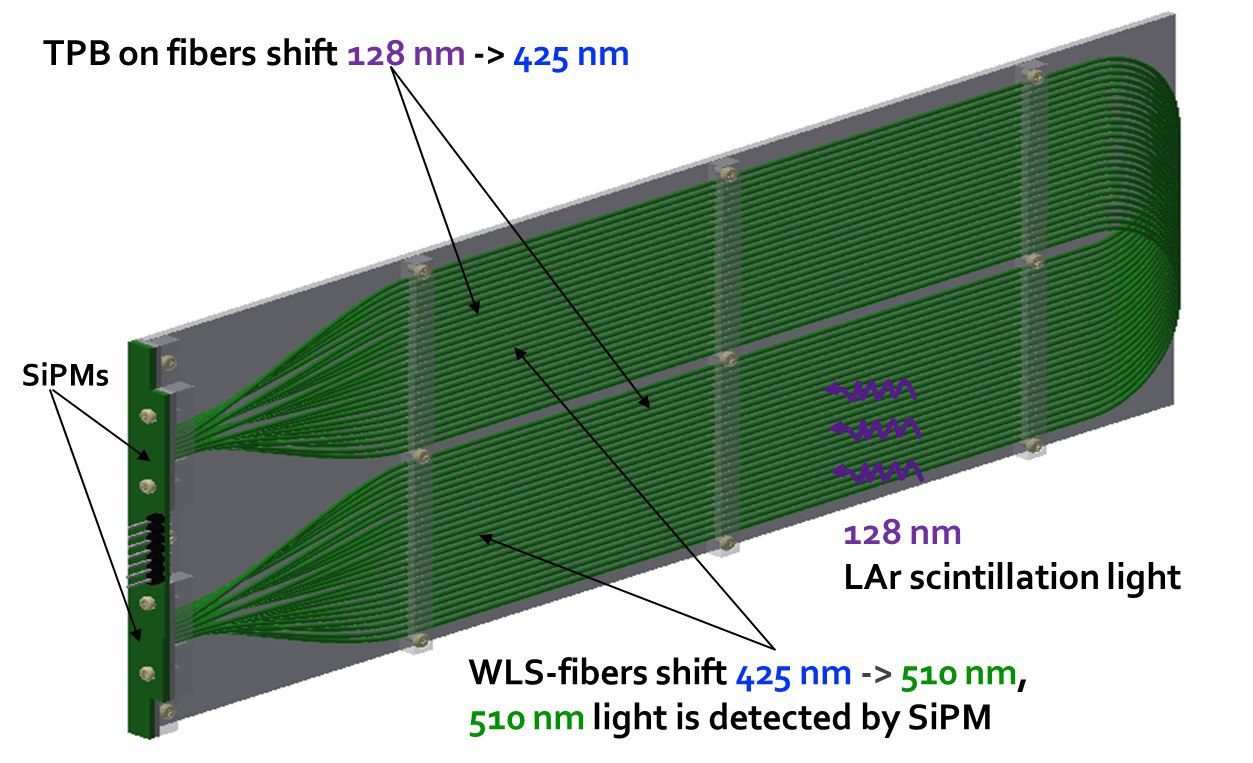
\includegraphics[width=0.5\linewidth]{graphics/lartpc/Light/lcm.jpeg}
\caption{\label{fig:fig_modules} Two approaches to light detection: Left – ArCLight, Right – LCM.}
\end{figure}


The Light Collection Module prototype is a frame cantilevered by a PVC plate that holds WLS-fibers which are bent into two bundles optically coupled to two SiPM light sensors (Fig.~\ref{fig:fig_modules}~right). The Fibers are grouped and held by spacer bars with holes which are fixed on the PVC plate by means of polycarbonate screws to provide matching of thermal contraction. The PVC plate with the WLS-fibers are coated with TPB that re-emit absorbed the VUV light (\SI{128}{\nano\metre}) to the violet ($\sim$\SI{425}{\nano\metre}). The violet light is shifted inside multi-cladding $\varnothing$=\SI{1.2}{\milli\metre} Kuraray Y-11 fibers to the green light ($\sim$\SI{510}{\nano\metre}) and hence is trapped by total internal reflection that guides this light towards to the fibers ends readout by SiPMs.  The LCM dimensions are \SI[product-units=repeat]{100x\sim500x10}{\milli\metre}.

\subsubsection{SiPM Readout}

SiPMs\footnote{e.g. Hamamatsu S13360-6025PE or S13360-6050PE} mounted on a Printed Circuit Board, are shown in Figure~\ref{fig:pcb}~right. The SiPM-PCB has \num{2} double-pin connectors to plug it onto an E-shaped readout PCB (E-PCB), shown in Figure~\ref{fig:e-pcb}~right, which drives 3 LCMs (6 SiPMs) or 1 ArCLight module (6 SiPMs). To gain signal from the SiPM a LMH6624 preamplifier from Texas Instruments is used. The E-PCB contains 6 preamplifiers to provide signal transition through the long coaxial signal line. Each preamplifier dissipates around \SIrange{60}{80}{\milli\watt} in a range of \SI{1}{\volt} and a bandwidth of \SI{30}{\mega\hertz} ($\sim$\SI{10}{\nano\second} rise time). Such an energy dissipation leads to LAr bubbling and requires E-PCB displacement outside the active volume behind the pixelated anode plane. Since there are two semi-TPCs in a single module, a left- and a right-handed E-PCB are used in order to provide a symmetric mechanical assembly (Fig.~\ref{fig:e-pcb}~right). 

To connect the individual E-PCB with the feedthrough board inside the TPC module the microcoaxial cable assembly is used. Each assembly consist of \num{20} micro-coaxial cables (38 AWG) by Samtec. Part number is FCF8-20-01-L-XX.XX-S, where XX.XX - is a length specified in inches. The cables are plugged into the FCS8-20-01-L-S-A-TR connectors by Samtec mounted both on the E-PCB, and on the feedthrough (see Fig.~\ref{fig:e-pcb}~right). On the warm side, to interconnect the feedthrough board with front-end electronics that placed  in the VME crates, the same type of cable assemblies and connectors by Samtec are used. 


\begin{figure}[htbp]
\centering 
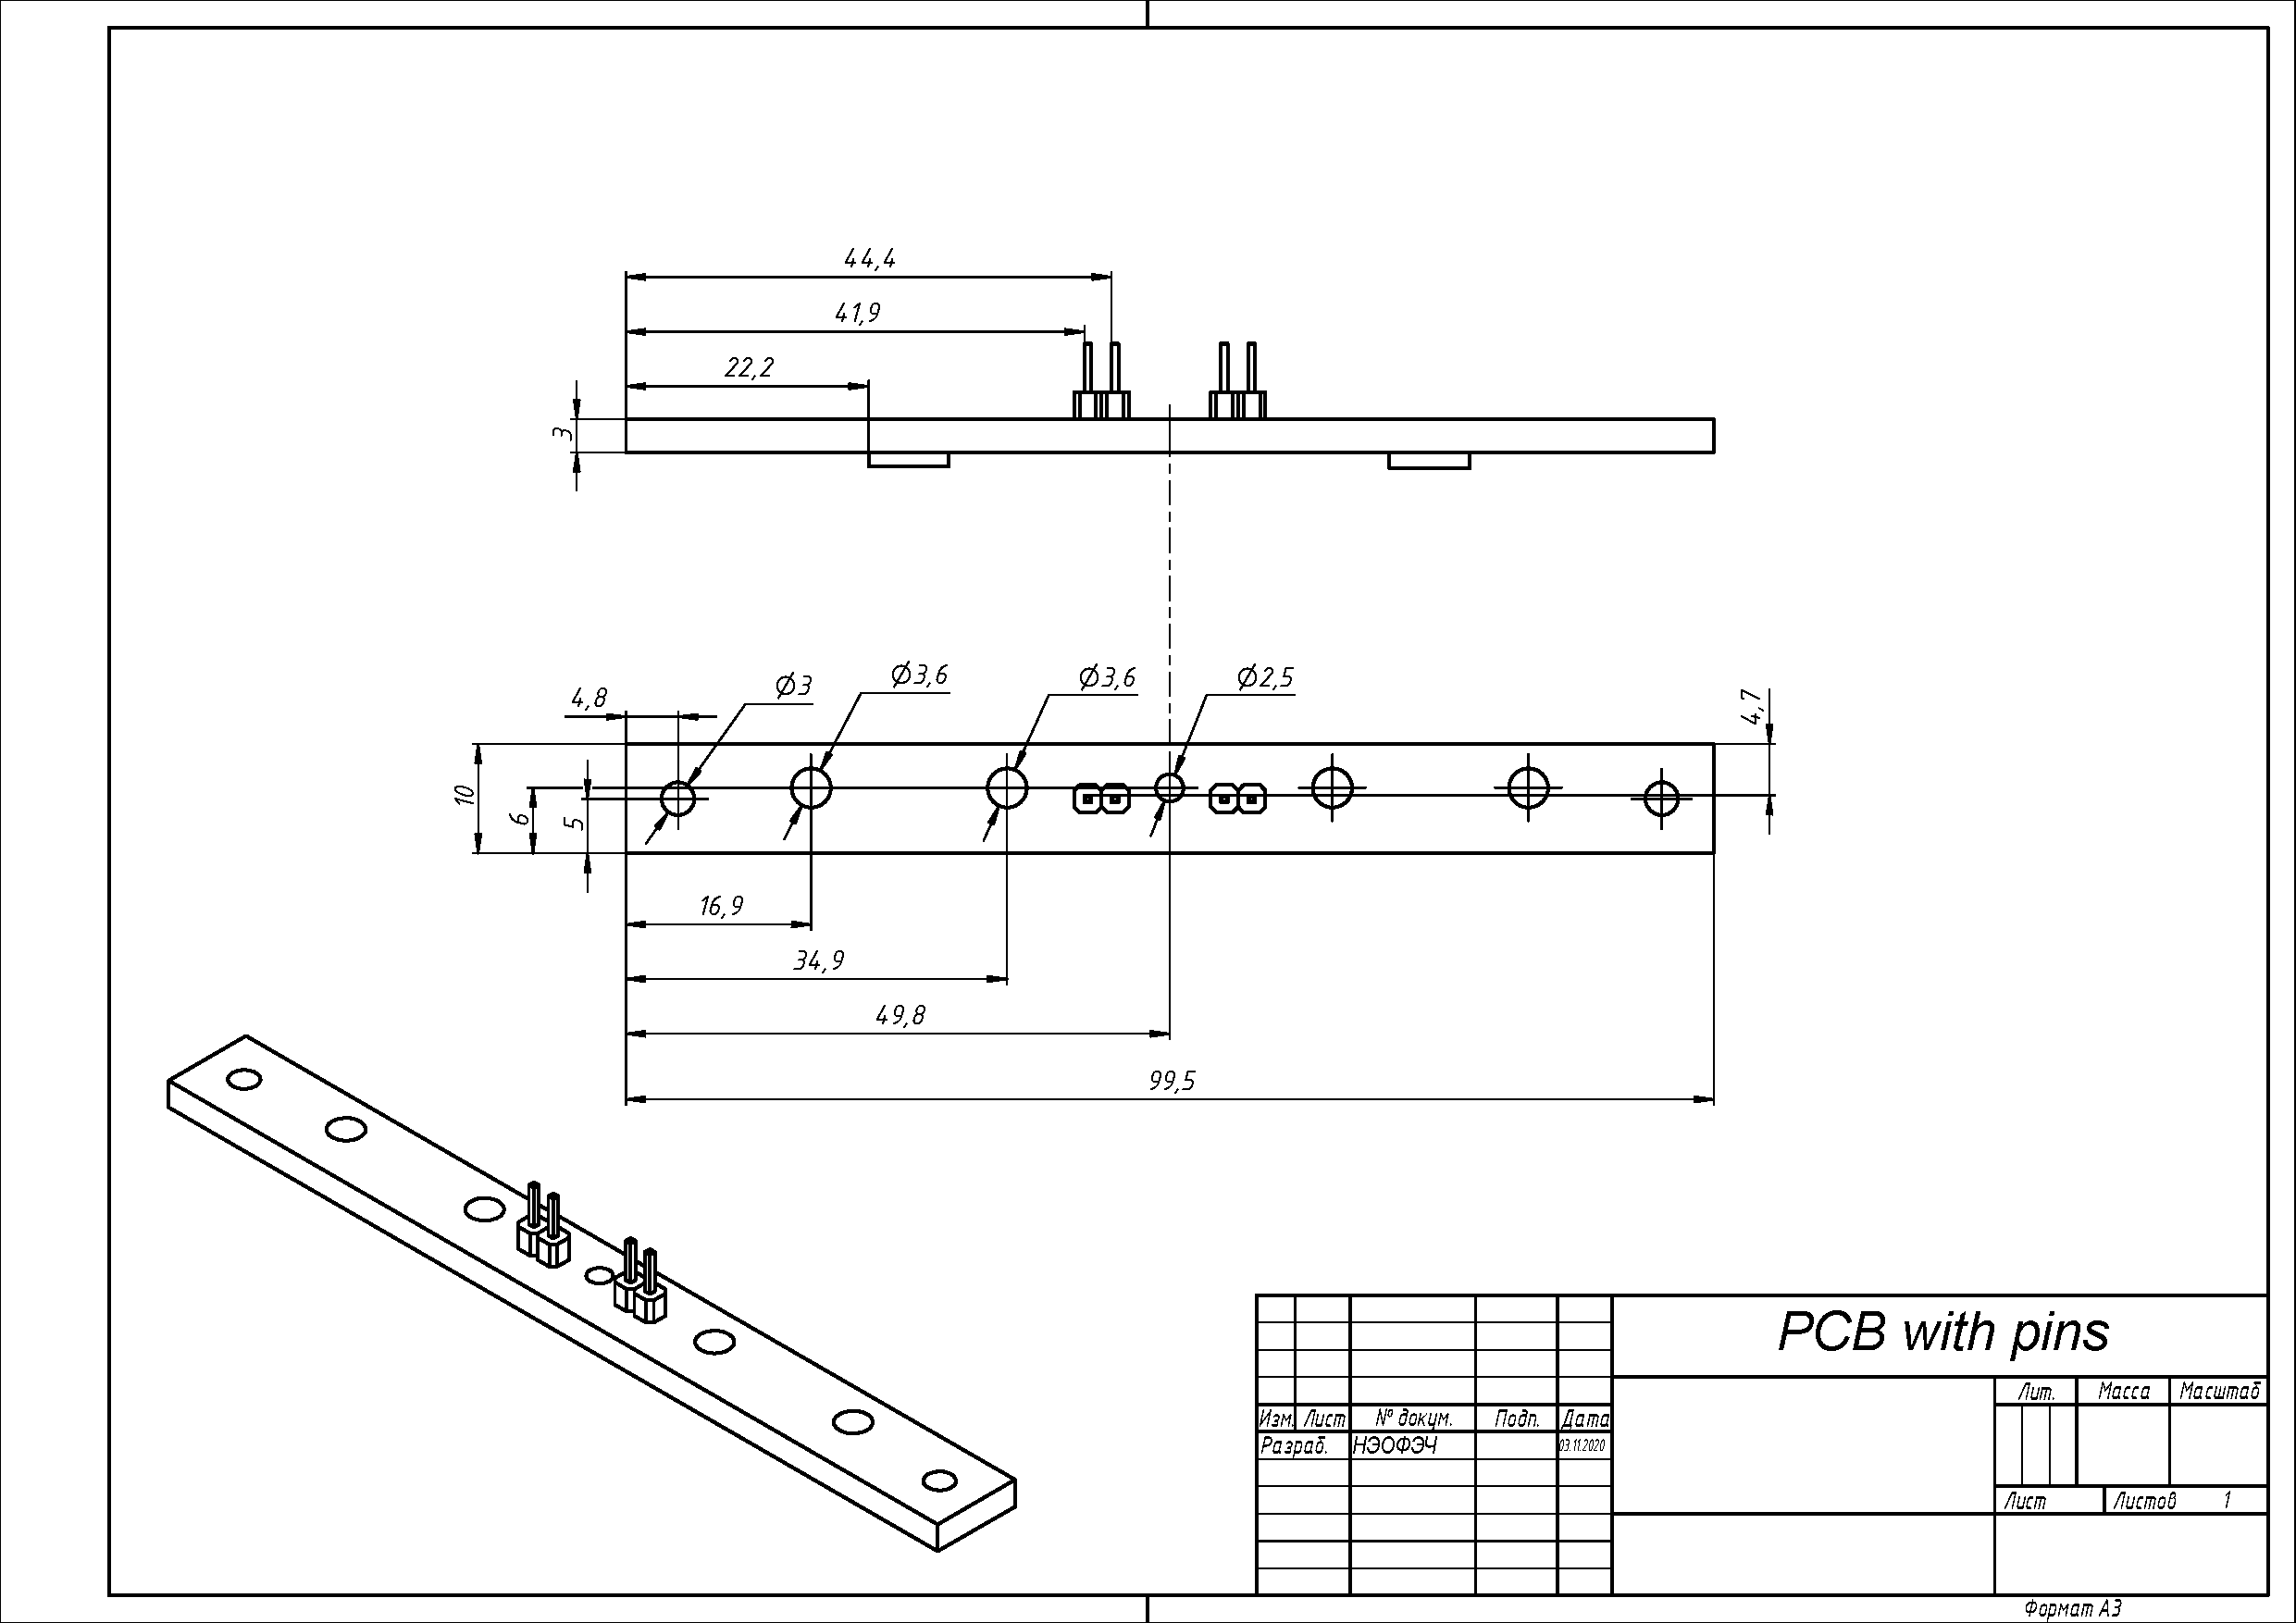
\includegraphics[width=0.47\linewidth]{graphics/lartpc/Light/SiPM_PCBdrawing.pdf}
\qquad
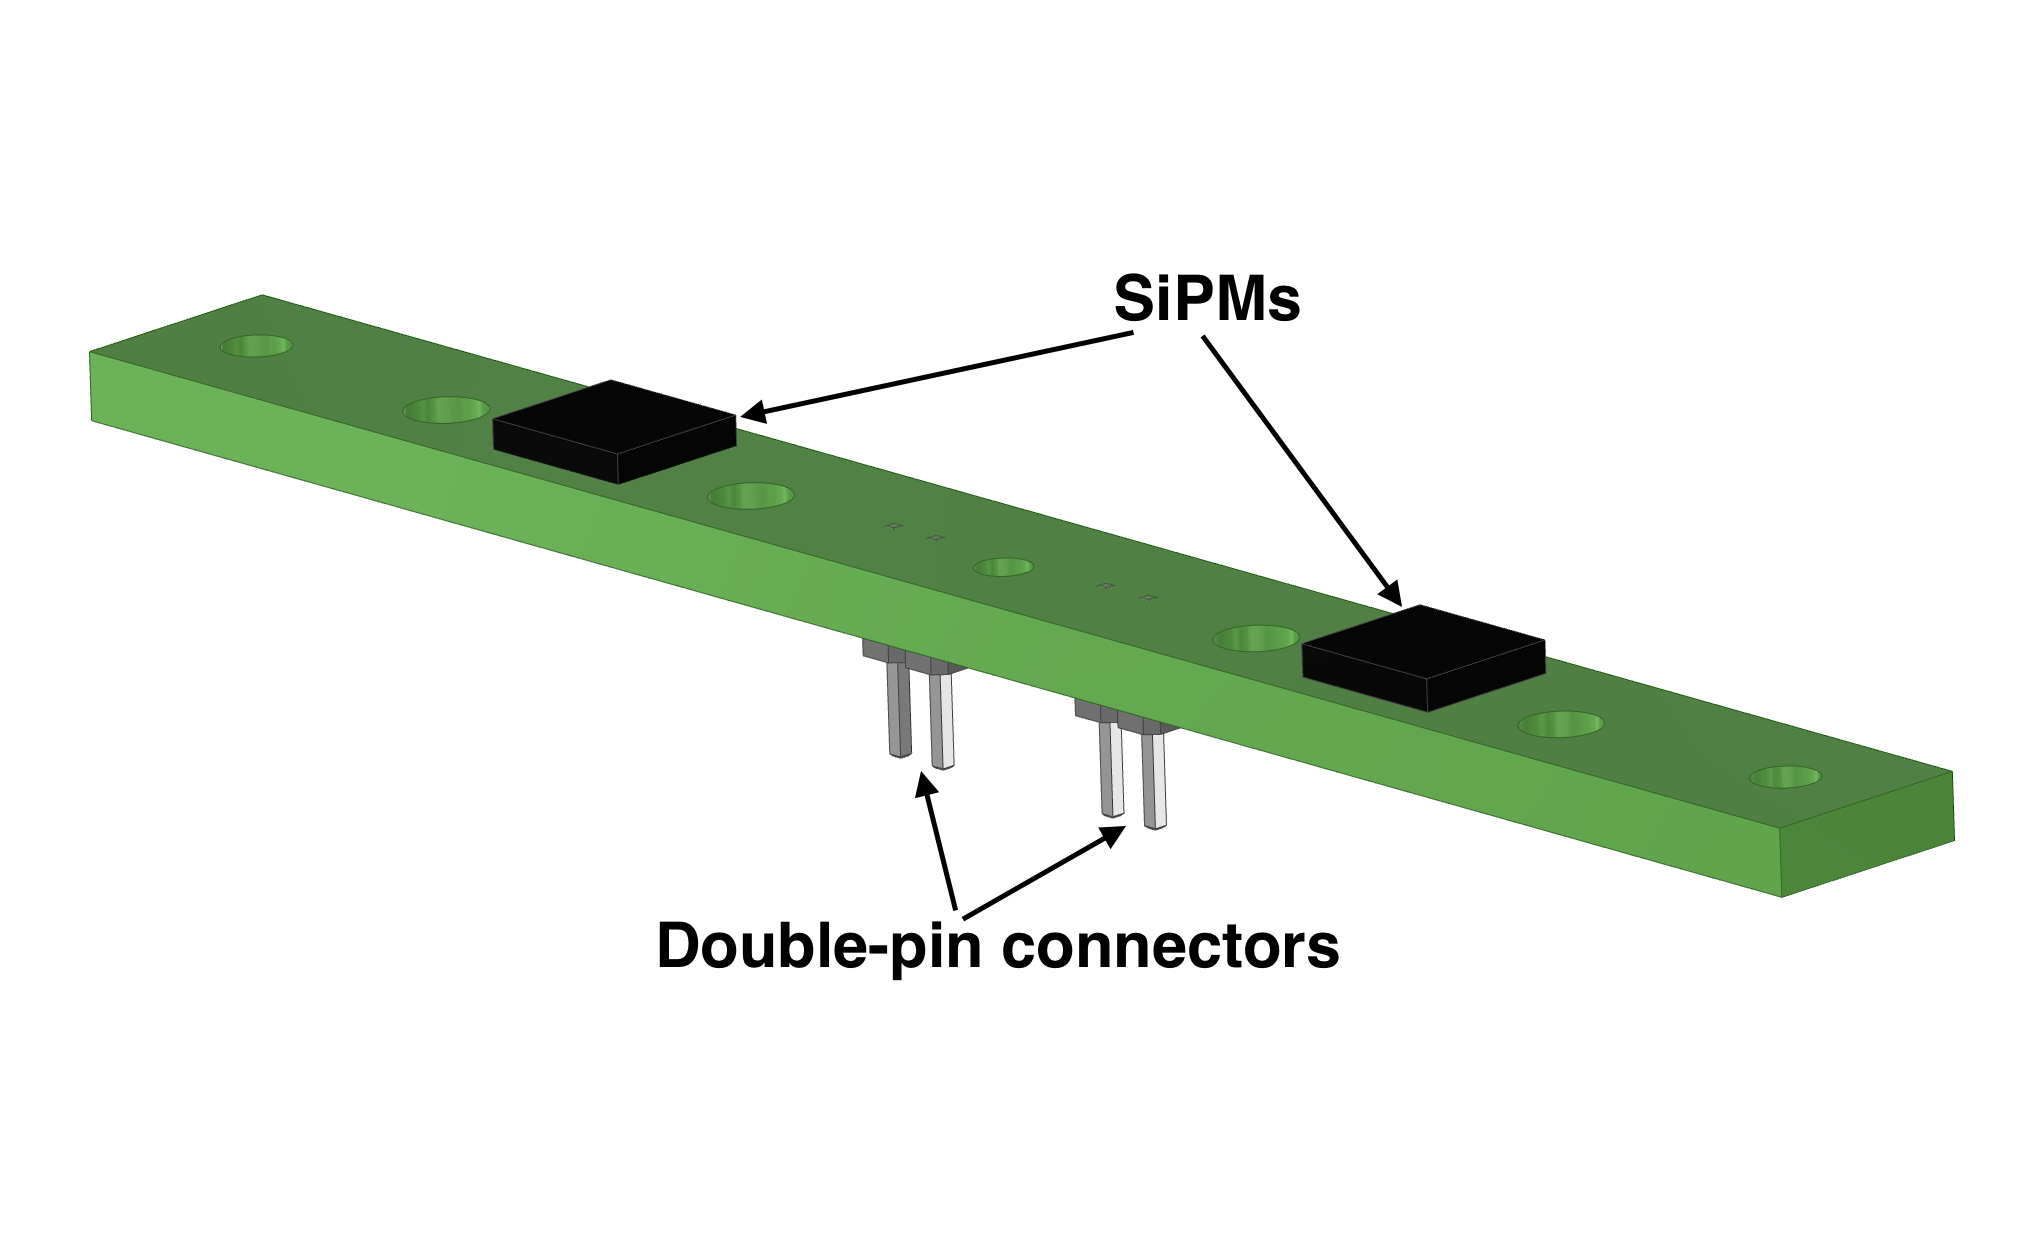
\includegraphics[width=0.47\linewidth]{graphics/lartpc/Light/SiPMpcb.png}
\caption{\label{fig:pcb} The SiPM-PCB drawing and general view. Numbers are given in units of mm.}
\end{figure}

\begin{figure}[htbp]
\centering 
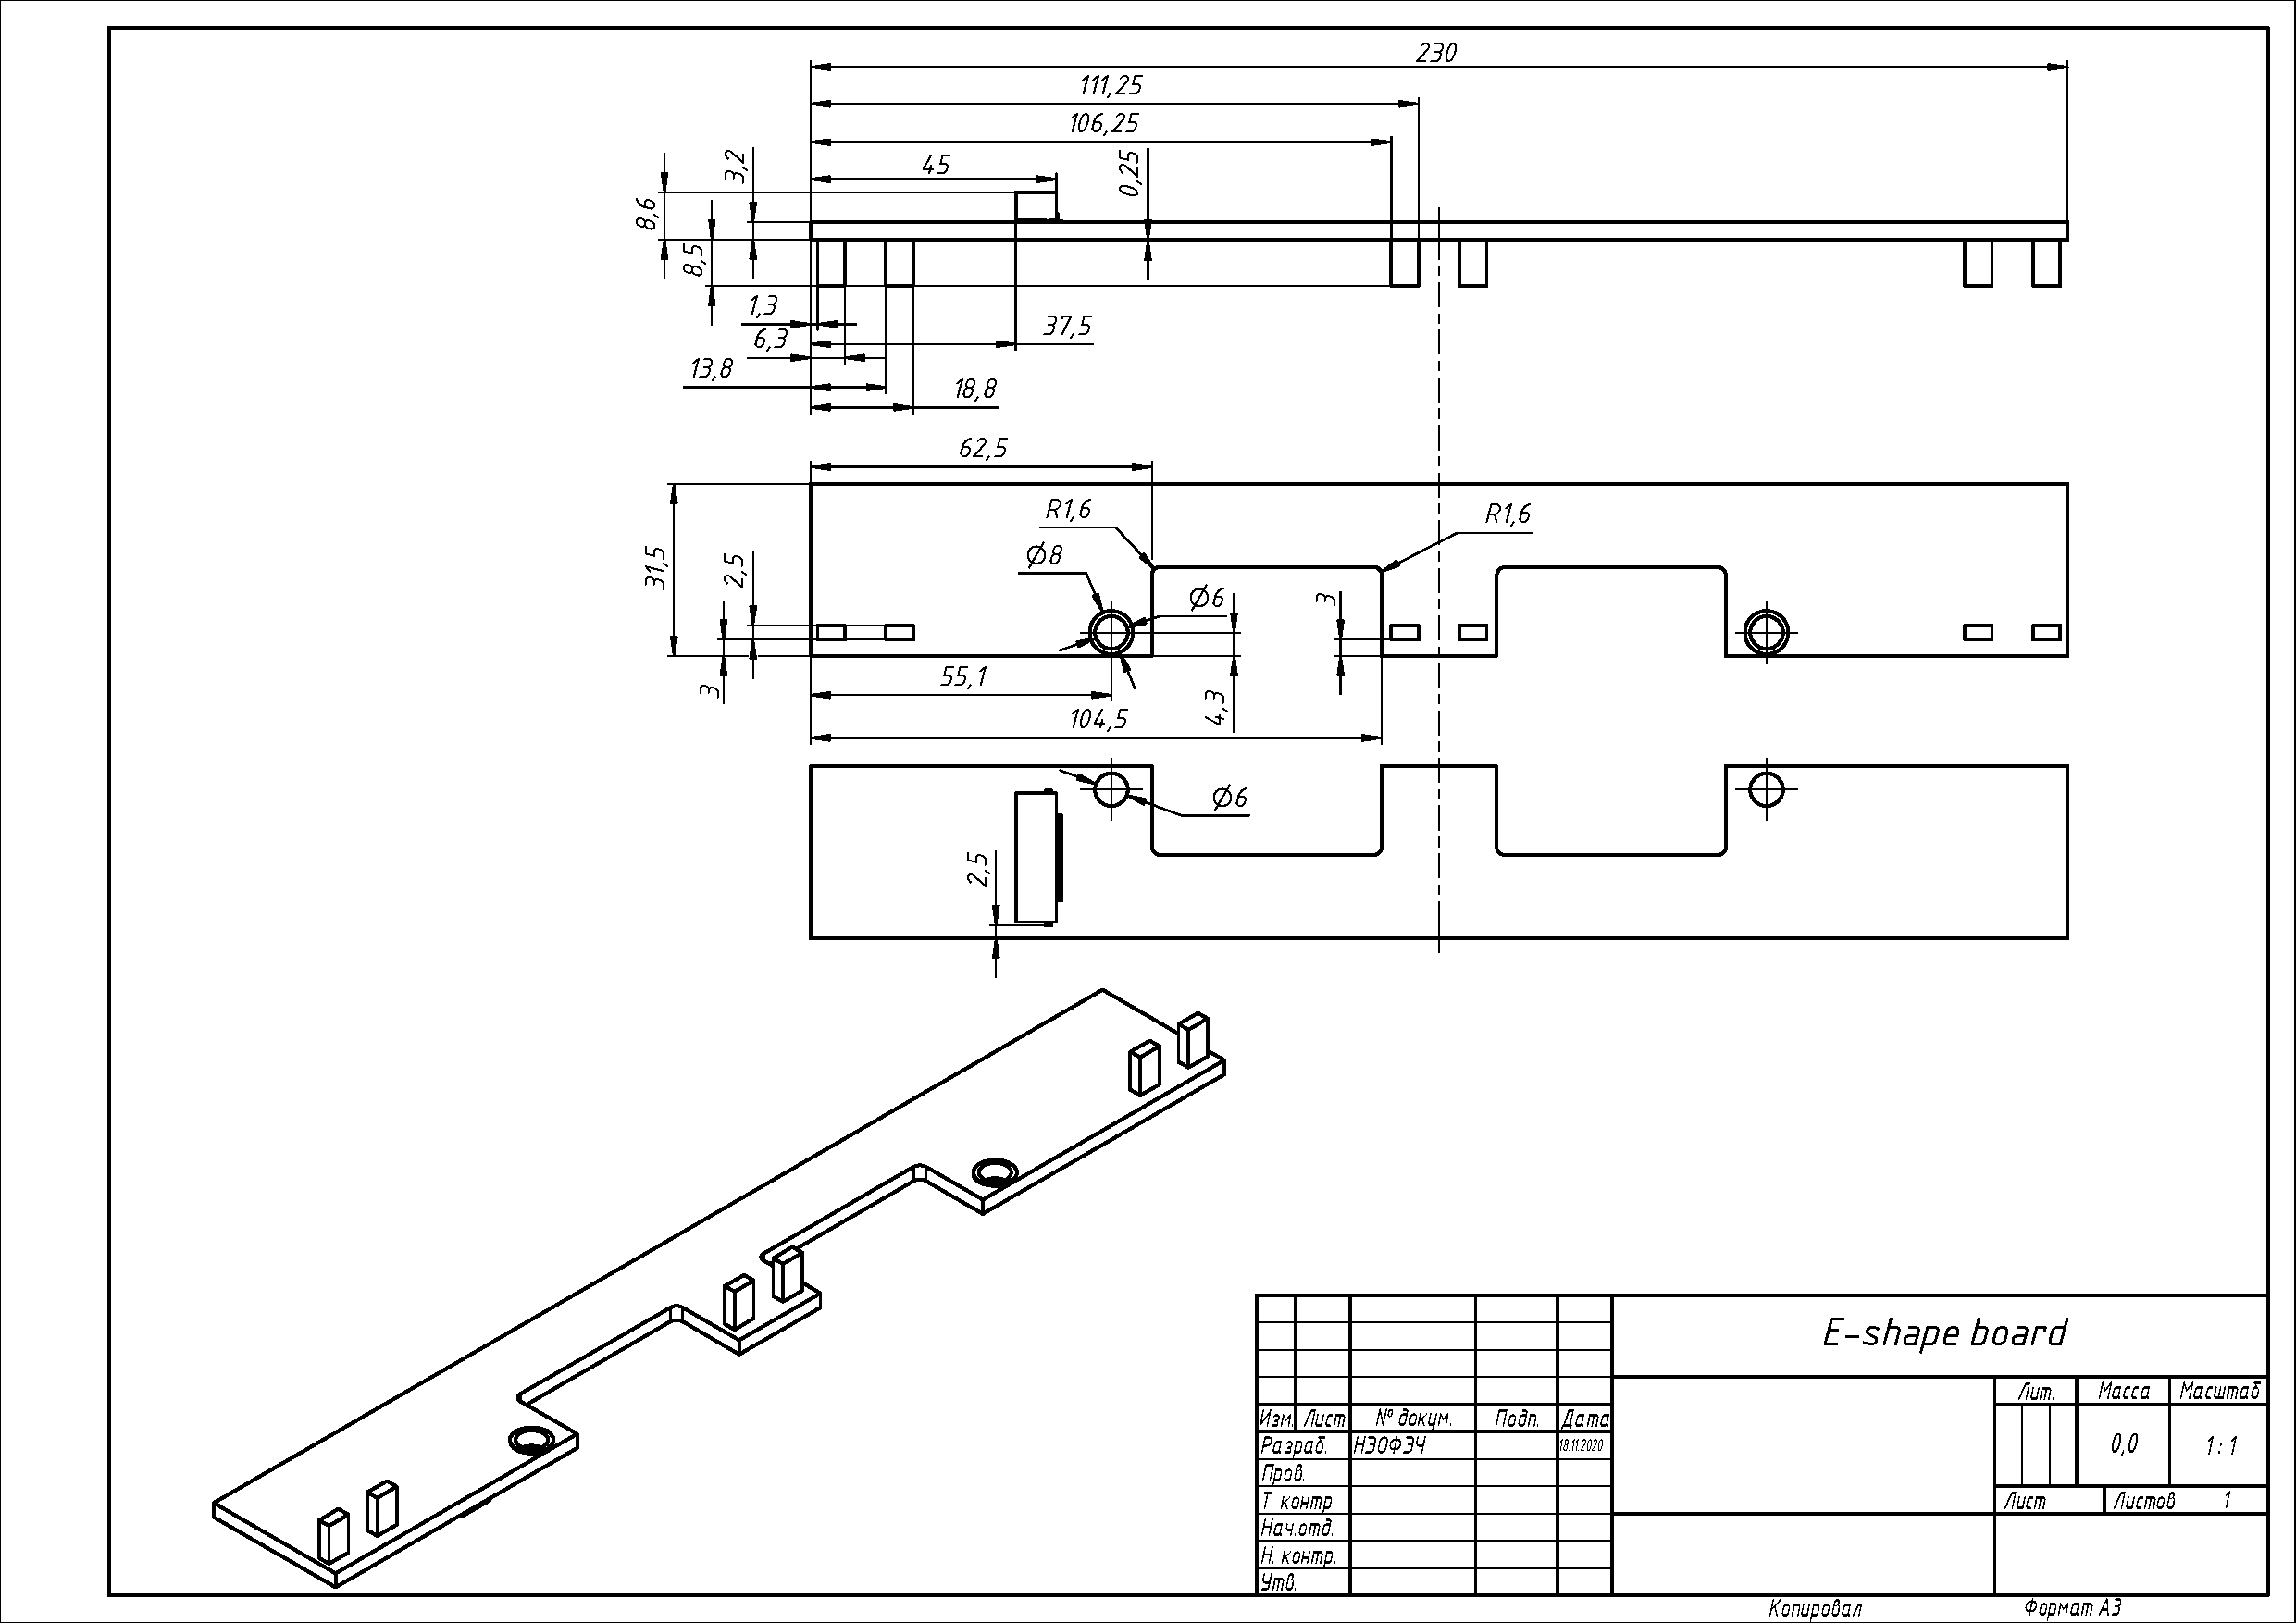
\includegraphics[width=0.47\linewidth]{graphics/lartpc/Light/Eboard.pdf}
\qquad
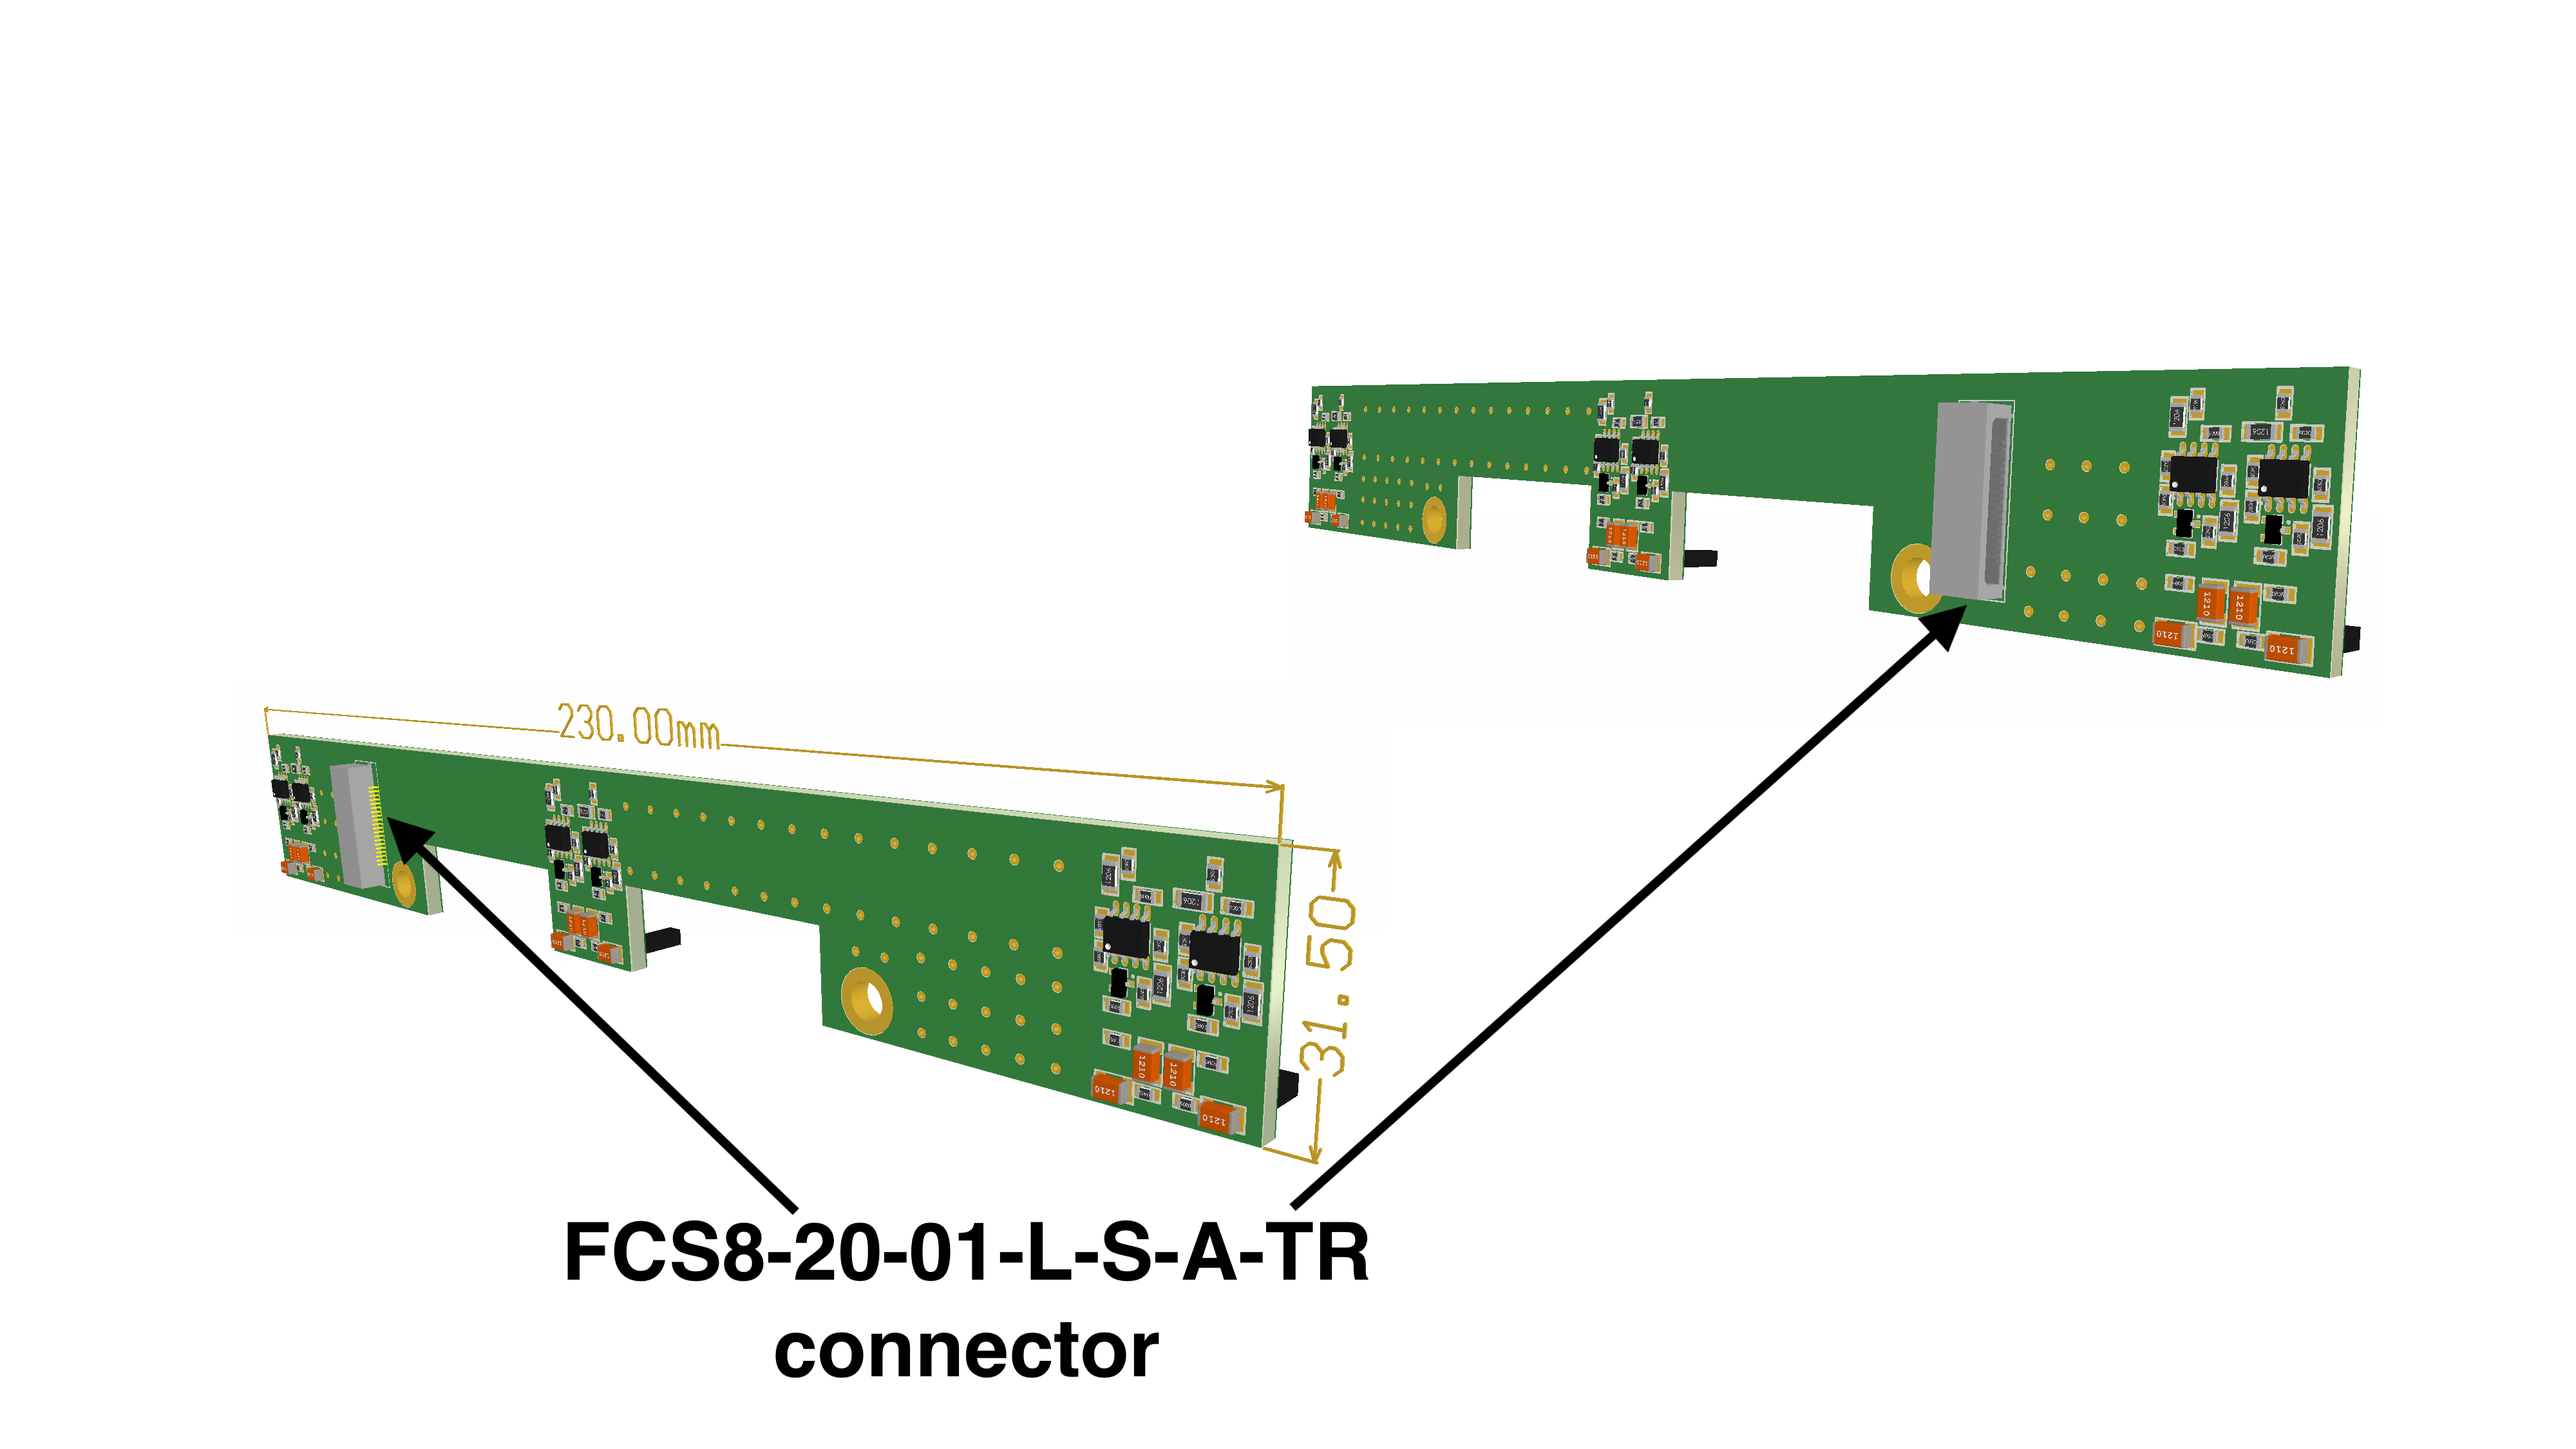
\includegraphics[width=0.47\linewidth]{graphics/lartpc/Light/EE.png}
\caption{\label{fig:e-pcb} The E-PCB drawing and the left- and right-handed E-PCBs (right). Numbers are given in units of mm.}
\end{figure}

\subsubsection{SiPM Power Supply}

For biasing the SiPMs with reverse voltage a power supply module based on the HV DAC AD5535 by Analog Devices is used. The module is a 6U VME card that composed of 4 HV DACs chips provides 128 power channels.  The light system of the single ND TPC has 240 SiPM photosensors and, therefore, they are supplied by 2 HV DAC cards. Each DAC card provides also monitoring and feedback for each DAC channel by means of multiplexers and ADCs that readout voltage dividers on each channel's output. Both DAC cards are placed in an individual VME 6U crate that manages the TPC module. Bias voltage that required for the considered SiPMs is up to 70 V (max). Common high voltage is distributed between 70 SiPM PS cards ($2\times35$ modules) is provided by a powerful laboratory voltage source (up to 1~A) which is enough to supply all the SiPMs of the entire light system. It is planned to place the HV laboratory source in the rack located at a distance from the ND. The rack might be shared with ADCs, trigger and timing system or some other electronics. Additional option is to embed a DC-DC converter  on the individual DAC card that provides the HV voltage for DAC by converting it from crate LV power\footnote{Both options are under consideration}.

\subsubsection{Front-End electronics}

The microcoaxial cable assemblies are used both for the signal transferring from SiPMs and to deliver the power for SiPMs and pre-amplifiers.These cables routing from the feedthroughs to the Patch board placed in the VME crate on top of each TPC module.  The Patch board is intended to split wires in cable assemblies to distribute power from the DAC boards, amplifier power supplies and deliver signals to VGA modules. Each VGA module has 24 channels of AD8264 by Analog Devices programmable variable gain amplifiers that can adjust the SiPM's signals to the input dynamic range of the ADCs while calibration of the SiPMs (single photoelectrons/low amplitudes) and high energy dissipations (high amplitudes). Each channel of VGA module is also equipped with  amplifier (ADA4938 by Analog Devices) that convert unipolar signal into differential line to the ADC by means of the long ribbon twisted pair cable. The module also form the sum signals from each E-PCB (6 ch)  that can be used for the  trigger production thereafter. Each TPC module has 240 SiPM channels that require 10 (in the case of 24 ch module) or 5 (in the case of 48 ch module) of the VGA module that are placed in the VME 6U crate (21 slots). This crate is also shared between 2 DAC modules, 1 patch board, 1 trigger module, and a Control module. Control module is a 6U PCB in VME standard currently is under development. It is supposed to be based on the module phyCORE-i.MX 7, or Freescale iMX287, or Raspberry Pi microcomputer and intended to control the gain of VGA PCBs and the voltage on the DAC PCBs via the CANopen communication protocol. Trigger module is a  6U PCB that produces required trigger signals to run the ADCs by utilizing the sum signals from VGA PCBs and provide external trigger mark for the charge readout system.

\begin{figure}[htbp]
\centering 
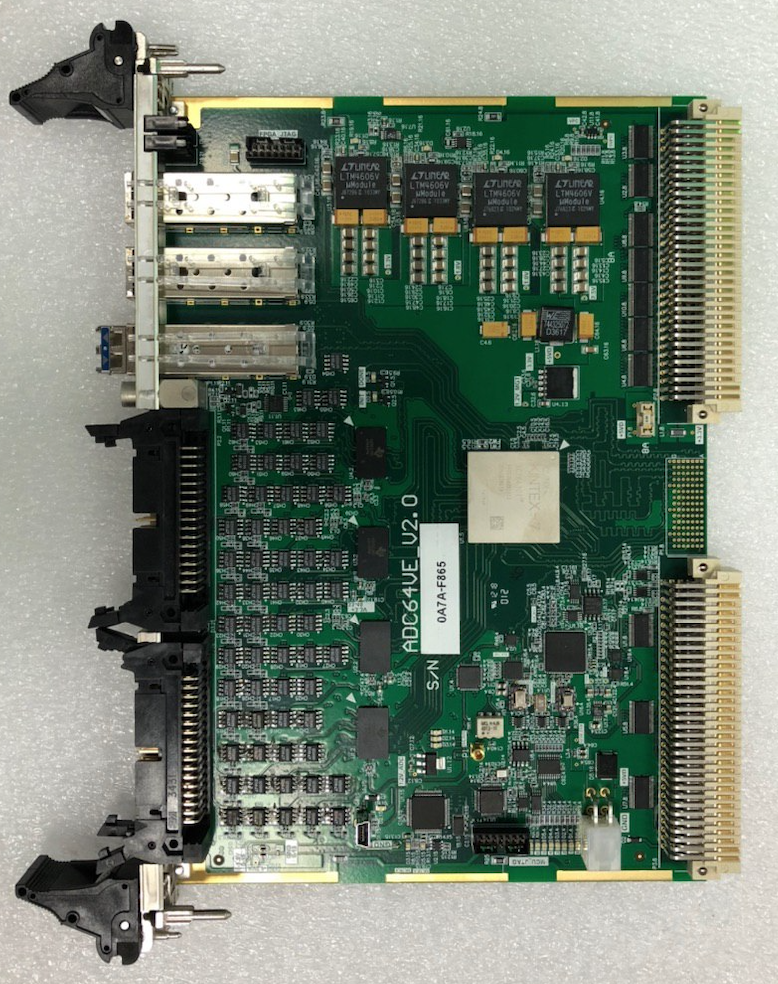
\includegraphics[width=0.4\linewidth]{graphics/lartpc/Light/adc.png}
\qquad
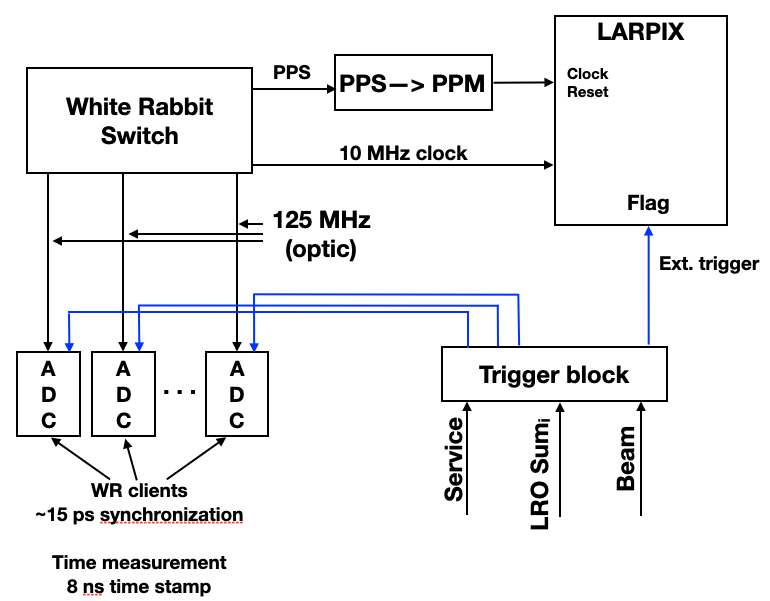
\includegraphics[width=0.52\linewidth]{graphics/lartpc/Light/sync.png}
\caption{\label{fig:adc} Left - JINR ADC board, Right - Synchronization scheme}
\end{figure}


\subsubsection{Data acquisition }

To digitize analogue signals from SiPMs a 100 MHz 10-bit 64-channel (differential signals, full range $\pm$~1.6~V) ADC module in VME standard produced by JINR AFI is used (see Fig.~\ref{fig:adc}~left). This ADC stream UDP/TCP data packets via M-link MStream protocol that provides 10 Gbps optical link. To provide the connection of ADC with the DAQ computer a Network 10 Gbps optical Switch with SFP+ ports is required. For 240 SiPM channels of the single TPC one require 4 ADCs, thus, 140 ADCs for the entire ND. There are two options for ADCs location. The First option is to put the 4 ADCs to the crate with front-end electronics on top of the individual TPC. The Second option is to place ADCs to the crate at some distance from the TPC module\footnote{e.g. in the racks supporting TPC rows}.

The synchronization scheme is presented in Fig.~\ref{fig:adc}~right. White rabbit\footnote{White Rabbit can obtain absolute time from GPS which could be a helpful option to synchronize both Near and Far detectors.} switch distributes 125~MHz clock via optical cables which tunes up 100~MHz clock of all ADC by means of PLL with subnanosecend precision. Ones all the ADCs are synchronized the system can associate light pulses with required precision of less than 10 ns. 
Each ADC board has WR-client and can measure time with 8~ns timestamp. Together with light readout the charge readout system is synchronized by 10~MHz clock distributed by WR main switch. Internal counter has 32-bit register which can count clock signals up to $\approx7$~min.  To exclude pileup in files roll over LARPIX PACMAN will convert PPS (pulse per second) coming from WR switch into a PPM (pulse per minute) which reset the counter. 
The scheme allows to provide the timing of event in charge readout much better than a clock time of 100~ns comparing to the level of 8~ns.
The trigger block will provide a common trigger logic for sum signals coming from light readout VGAs within the beam spill. This signal runs ADCs readout and marks clock number in LARPIX associated with Light trigger. To exclude delays on signal line trigger block will be equipped with precision TDC~(25~ps).


% \subsubsection{Performance tests and evaluation}

% Several light readout prototypes (LCM/ArCLight with some electronics) with reduced light detector dimensions (300 cm length) were built and tested so far. Tests were performed at Bern University and in Dubna. Preliminary results have confirmed expected specifications that will be studied more detailed in the upcoming tests of SingleModule and 2$\times$2 Demonstrator. Current light readout concept is considered as a baseline for the final system and probably will be slightly modified after the review. 

\subsection{Calibration}
\label{sec:lartpc-des-calib}
%{\it Kendall/Jelena. 3 pages}

\subsubsection{Introduction} 
The DUNE Near Detector overarching requirements and overall physics goals cannot be achieved without thorough understanding and characterization of the Near Detector LAr TPC. The ND LAr TPC’s performance in terms of energy and vertex resolution, momentum and angular track resolution, particle identification and reconstruction, must at the minimum match the performance of the DUNE Far Detector. Contrary to DUNE Far Detector, DUNE Near Detector will collect an enormous statistics and its measurements of the neutrino flux, extrapolation of its measurements to FD, and measurements of neutrino cross-sections will be dominated by its systematic error budget. It is imperative that the overall systematic error of the ND measurements and their extrapolation to FD, are subdominant in the overall DUNE error budget and do not negatively influence it. Calibration of the Near Detector is at the heart of reaching  this goal. The calibration program must provide measurements and verify detector performance at a few percent or better level, with sufficient spatial granularity, with respect to detector movements and over the lifetime of the detector. 
\subsubsection{Calibration Key Requirements}
\label{sec:lartpc-cal-req}

The key driving design requirements and performance requirements for the field structure are summarized in Figures~\ref{fig:lartpc_cal_req1},and \ref{fig:lartpc_cal_req2}. 

\begin{figure}
\centering 
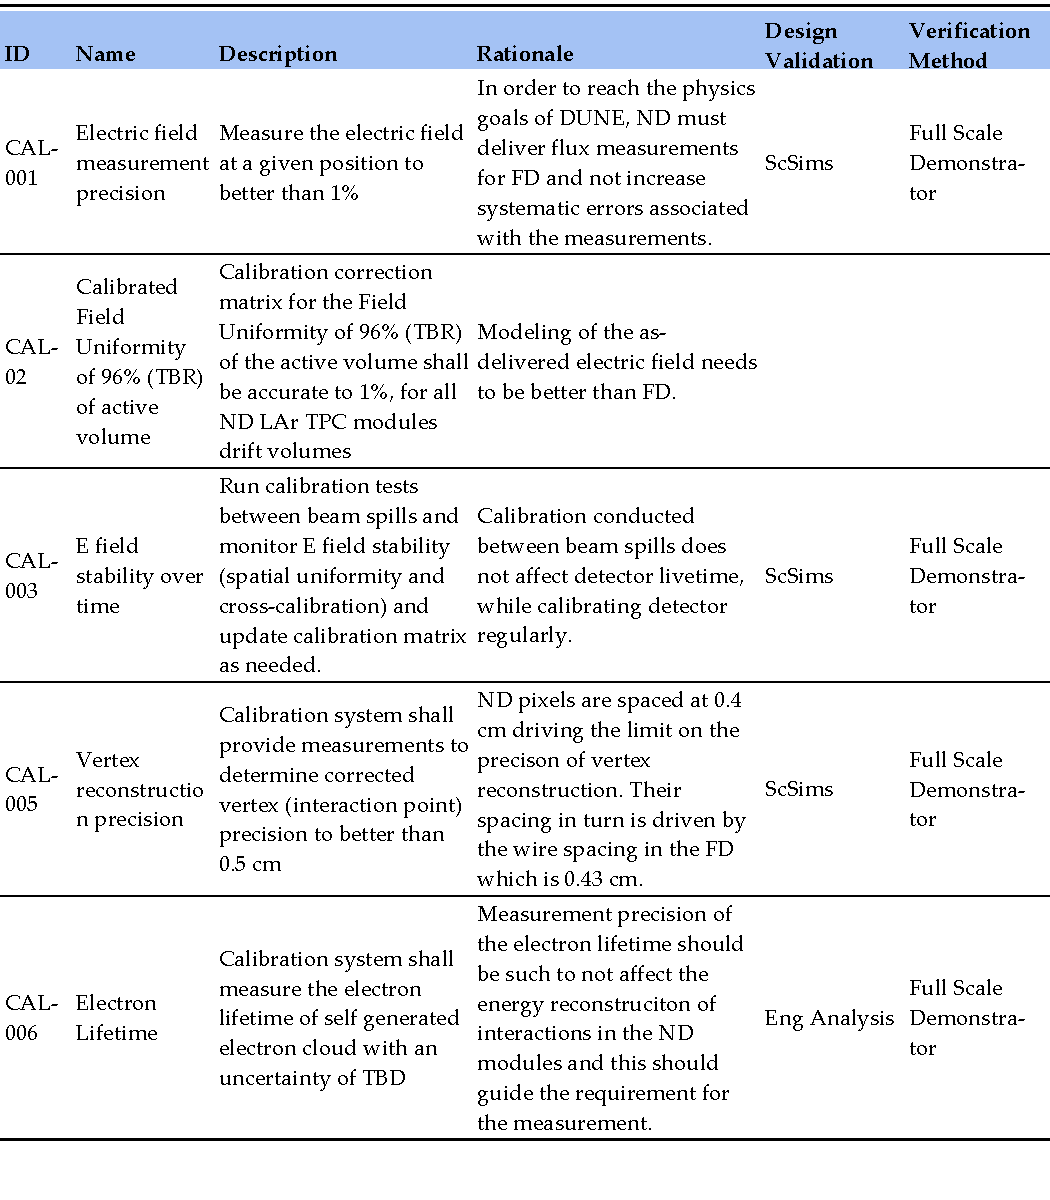
\includegraphics[width=1\linewidth]{graphics/lartpc/0Req/NDCalreqs1.pdf}
\caption{\label{fig:lartpc_cal_req1} ND LArTPC Key Calibration Requirements (1)}
\end{figure}

\begin{figure}
\centering 
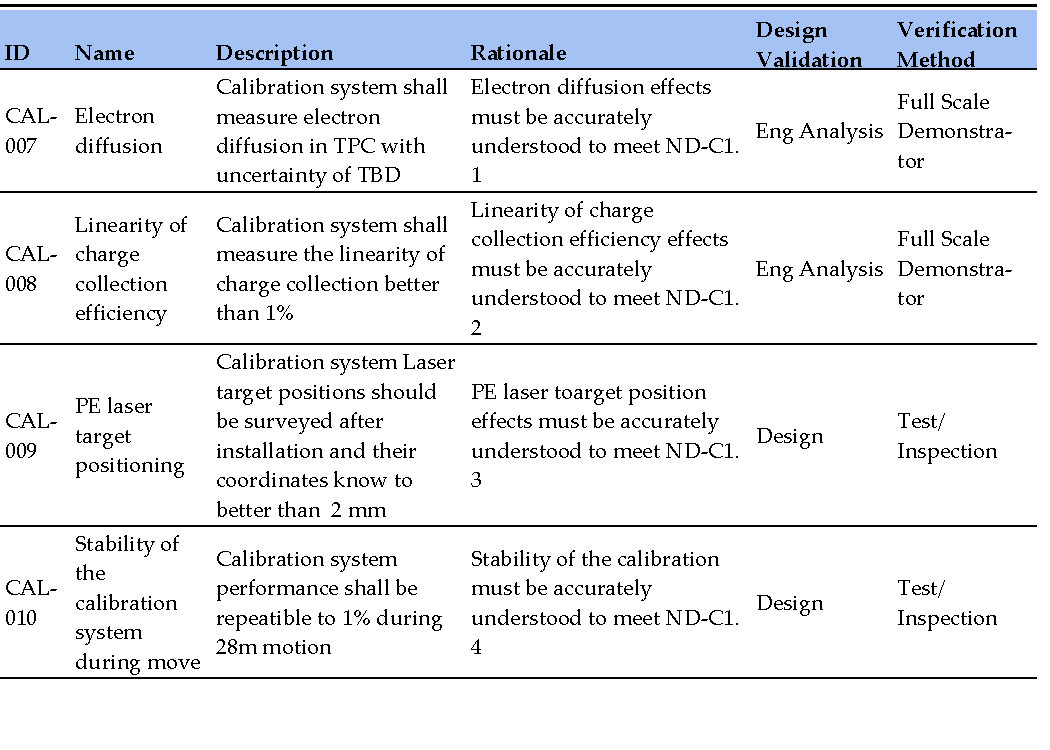
\includegraphics[width=1\linewidth]{graphics/lartpc/0Req/NDCalreqs2.pdf}
\caption{\label{fig:lartpc_cal_req1} ND LArTPC Key Calibration Requirements (2)}
\end{figure}

The Near Detector calibration program will rely on both dedicated systems and natural sources to perform calibration. Natural calibration sources include cosmic rays, rock muons and argon isotopes such as $^{39}Ar$. Given the stringent requirements for the overall ND-induced systematic error that requires finely grained spatial calibration, rock muons and other natural sources lack the quality required to meet the ND calibration goals. Thus, dedicated calibration hardware systems are required.  Calibration hardware systems under consideration include photoelectron (PE) laser system and embedded radioactive sources (beta emitters). These systems measure the detector response model parameters and verify the validity of the detector response model. Employment of different techniques will provide constraints on detector associated systematic errors, including detector cross-calibration between different TPC modules, detection efficiency uncertainty, linearity of the response, and stability of the response through detector movements and over time.

\subsubsection{PE Laser System}
Purpose of the PE Laser System
        Well localized electron sources represent excellent calibration tools for the study of electron transport in the LArTPC. A photoelectron laser system can provide such sources at predetermined locations on the cathode, leading to precise measurements of:
        
\begin{itemize}
        \item
    the total drift time and charge drift velocity at predetermined locations on the cathode
    \item
    space charge effects at various positions in the detector
    \item
    position reconstruction close to cathode
    \item
    Measurement of diffusion effects for charges traveling the full  drift                 ,
    \item
    Charge collection efficiency
    \item
    Charge trigger threshold
\end{itemize}

\subsubsection{Key elements of PE Laser}
In order to produce localized clouds of electrons using a photoelectric effect, small metal discs will be placed on the cathode and used as photoelectric targets. Photoelectric targets are illuminated by diffused 266 nm wavelength light  generated by the Nd:YAG laser quadrupled wavelength to produce localized electron clouds. Laser light pulses are injected into UV optical fiber bundles outside the cryostat, brought in through the flange and then distributed to each TPCs module via cryogenic UV optical fibers. Fig. \ref{fig:PElaser_overview} illustrates the light injection scheme.

\begin{figure}[htbp]
\centering 
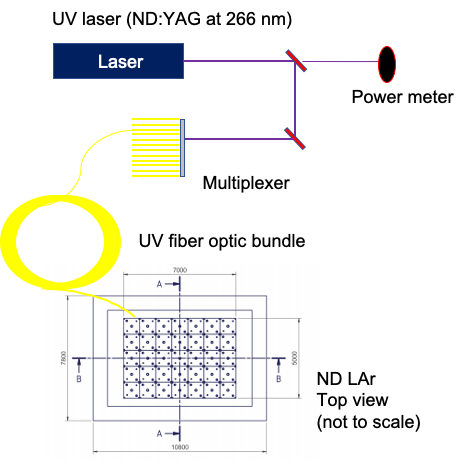
\includegraphics[width=0.47\linewidth]{graphics/lartpc/Calibration/PElaserOverview.png}
\caption{\label{fig:PElaser_overview} The An overview of the PE laser calibration system. NdYag laser light injected into optical fibers is guided to each TPC module for calibration.}
\end{figure}

\subsubsection{Major requirements that drive PE Laser design}
        
PE laser design is driven by the need for the precise calibration of particle energy and position inside the TPC, need to cross-calibrate detector response among all modules, as a function of time and especially after the PRISM related movements of the ND LAr cryostat. Specifically, these include precision measurement of the E field strength in the direction of the drift and transverse to it, with high granularity and over time.  Consequently, the system must accommodate low level calibration such as cathode plane tilt, electron lifetime, electron diffusion and linearity of charge collection efficiency.

\subsubsection{PE laser calibration  details}
   
Photoelectric laser system consists of the following parts: 266 nm ND:Yag laser, optical fibers, optical diffuser at the end of the fiber tips in the modules and photoelectric targets on the cathode wall of the TPC module. Targets will be mounted on both sides of the cathode to calibrate both fiducial volumes in each module.  The baseline material choice for the metal targets is aluminum, while silver is being considered as an alternative. At 266 nm (Nd:YAG quadrupled wavelength) the single photon energy of 4.66 eV is sufficient to generate photoelectrons from aluminum and silver, since the work function of aluminum is 4.06 eV and 4.26-4.73 (lattice dependent) for silver. However, aluminum and silver are prone to oxidation. In the case of aluminum, a thick layer of aluminum oxide forms on the surface, but this does not increase the work function of the material. The main factor driving the electron yield from the photoelectric targets is the quantum efficiency of the material. Although electrons will be released from the metal whenever photons hit the metal surface, most of the ejected electrons carry forward momentum and therefore are never released from the metal. Only a small fraction of released electrons back-scatters or knocks another electron out of the surface. The quantum efficiency for various metals is typically between 10-5 and 10-6 , thus quite low. All material candidates will be studied in the lab to verify the electron yield, and tested in the prototype module in order to verify the quantum efficiency for different materials.

\subsubsection{Component descriptions, counts per module/detector}
        
Opposite from the laser and fibers that will be procured through the vendor, PE targets will be custom designed to meet ND LAr Calibration requirements.
        
Disc targets will be fabricated with two different diameters: 2.5 mm and 5 mm to provide a test of the vertex reconstruction precision. In addition to circular targets, metal strips 0.5 × 20 cm are being considered to calibrate the rate of transverse diffusion in LAr. However, their impact on the cathode field will be carefully studied before being incorporated into the target list, to prevent any disruptions to the cathode electric field. The targets will be fastened to cathode by a type of cryogenic, adhesive film. Ideally, circular targets will be distributed along the edges, every 10 cm where distortions to the E field and TPC shape exhibit largest fluctuations. In the interior of the cathode, circular targets should be placed every 20 cm. In addition, slanted target strips will be fastened to the cathode. Strips should be placed evenly roughly every 40 cm in two rows for a total of 14 strips per one cathode side.  Fig.~\ref{fig:target_layout} Illustrates distribution of circular and strip targets on the cathode. The cathode will have targets on both sides in order to calibrate both volumes of each TPC module. 
        
\begin{figure}[htbp]
\centering 
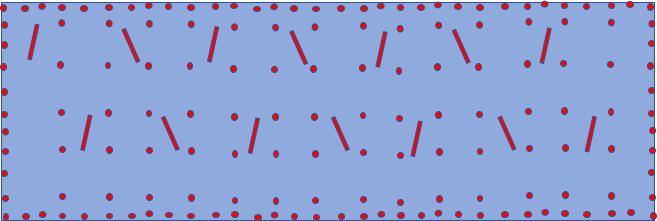
\includegraphics[width=0.47\linewidth]{graphics/lartpc/Calibration/PhototargetsCathode.png}
\caption{\label{fig:target_layout} PE target layout on the cathode surface.}
\end{figure}

 The laser beams used to illuminate the targets will be injected into the cryostat via cryogenic optical fibers guided inside each TCP module. The mounting points will be in the corners where the field cage and anode meet in order to illuminate the cathode across drift volume. There will be a minimum of 3 injection fibers illuminating each side of the cathode for a total of  6 fibers per module and 210 fibers per ND LAr. Fiber tips  will be coupled with defocusing elements that will illuminate 1x1 m2  area surface on the cathode with a single fiber. 
While the current plan aims for illumination of the entire cathode, the Kapton material that composes the resistive panels undergoes photoelectric effect, albeit with three orders of magnitude lower quantum efficiency at cryogenic temperatures when compared to phototargets at 266 nm. The noise produced is expected to be tolerable, but in case the noise is higher than anticipated, the solution is to illuminate only the areas where phototargets are placed, reducing the resistive panel exposure. In this case, instead of defocusing elements, bare fibers will be utilized. The bare fiber opening angle is 10° with a narrower exposure. Lasers typically operate at 10 Hz frequency. If 10000 pulses per laser are assumed, about 15 minutes of running is needed per laser for a single calibration run as the photoelectron clouds from different dots are very well localized. With the help of commercial multiplexers, 1 hour would be sufficient for a single calibration campaign. If the DAQ or lasers themselves prevent parallel running, the entire calibration campaign will take between 15 minutes or up to 1-5 hours. The calibration run duration will depend on the final calibration scheme. The photoelectron system will use the same NdYAG laser quadrupled pulse lasers used for argon ionization. Stability of the laser pulses will be monitored with a power meter. Dielectric mirrors reflective to 266 nm light will guide the laser light to injection points, but a fraction of the light will be transmitted instead of reflected to the power meter behind the mirror. The laser will also send an external trigger signal to the DAQ based on the photodiode that will combine the information with time stamps coming from self triggering of the pixels,  on the fraction of the light passing through the dielectric mirror.

      %  \item Figure: CAD of subsystem elements}
\subsubsection{PE  interfaces (mechanical, electrical)}
PE laser calibration system interfaces with various systems. In order to guide optical fibers inside the cryostat, the PE laser system interfaces with a cryostat, and each module. 
Since PE targets are placed on the cathode there is an interface with the cathode plane. 
        
There is also interface with the DAQ as it needs to accommodate calibration data obtained by the PE laser.
%\subsubsection{Component production}
%\label{sec:lartpc-cal-prod}        
%\subsubsection{Prototyping results}
%\label{sec:lartpc-cal-proto}        
       % \item Component specifications
       % \item Component production process
       % \item Prototyping results / spec validation
   % \end{itemize}

\subsection{Module Structures}
\label{sec:lartpc-des-modstruc}
%{\it James, 3 pages}
%%%%%%% dump from request, this is way out of format, but hopefully there is something useful I can build on.
Subproject A: Module structure and integration facility
\subsubsection{Overview}

The module structure is the connection between the TPCs and the cryostat. It provides the feedthroughs and routing of all infrastructure to and from the detector including: HV, argon (gas and liquid), readout signals, instrumentation (temperature and level). Thus, the module structure provided the interface requirements for the design of LBNF near site cryogenic infrastructure, as well as all other detector subcomponents.

Fig. 13: Illustration of the module structure above the TPC
As it is important to minimize material near the active volume, the module structure is used to provide structural integrity to the TPCs, allowing the the TPCs to be constructed form as little material as possible. This maximises the detectors active mass by moving structural components away from the active volume.
The module structure must locate each TPCs to a high precision with respect to its neighbouring TPCs. This is important when installing module rows into the cryostat. It is also vital for maintaining the required clearances and orientations during the cool down and operation in liquid argon, in order to minimize any uncertainties when reconstructing events across multiple modules.
The structure is itself modular by design in order to allow individual modules to be tested prior to their integration into a row of 5 modules. This is required for module transportation and handling as the TPC is not a sufficiently  rigid body to support itself without the structure above it. This also reduces the requirements on local test facilities, as a single 3 x 1 x 1 m3 module is significantly easier to handle and than a full row of five. This allows for commercially available cryostats to be used for testing individual modules prior to their integration.
\subsubsection{Module Structure Key Requirements}
\label{sec:lartpc-mod-req} 

The key driving design requirements and performance requirements for the field structure are summarized in Figure~\ref{fig:lartpc-mod-req1}.

\begin{figure}
\centering 
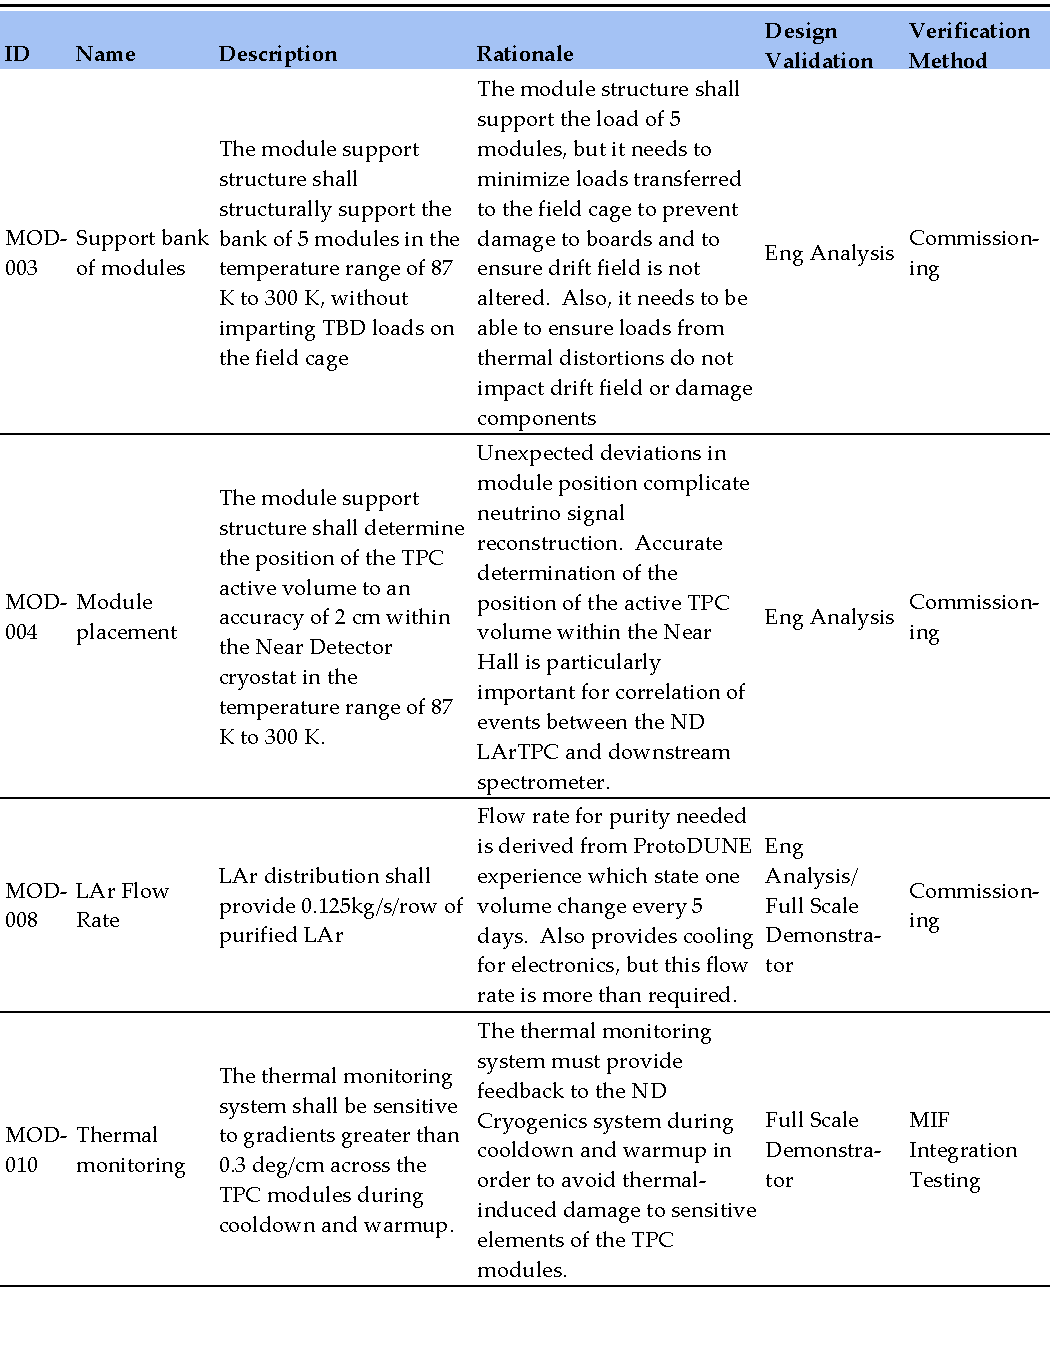
\includegraphics[width=1\linewidth]{graphics/lartpc/0Req/NDModreqs1.pdf}
\caption{\label{fig:lartpc-mod-req1} ND LArTPC Key Module Structure Requirements}
\end{figure}


\subsubsection{Status of module structure}
The module structure is in the initial design phase, key components have been identified and are being optimized based on the availability of standard industrial components and engineering analysis of all custom components. 
The design builds upon what was developed for the 2x2 demonstrator. 

Structural components: Considering a row of five modules, the cryostat lid above the row is  a section of membrane cryostat  5.7 m long, 1 m wide and 0.8 m deep. I-beams forming the external structure of the cryostat are mounted to the upper edge of this section. Eight titanium support ties pass through the membrane and tie the I-beams to a 25 mm thick steel plate that spans the area below the membrane. This steel plate provides the fixing point for the modules to be mounted to.  Above each module is a square steel frame that is attached to the TPC to provide structural rigidity to the module, this frame is precisely located on and then bolted to the fixing plate below the membrane. These frames are also used to support individual modules during testing and installation. The eight titanium ties, steel fixing plate, and five steel frames form the structural components. 

Fig. 14: Structural components above the modules: eight titanium ties connecting a steel fixing plate to the external I-beam structure.

Feedthroughs: There are feedthroughs above each module providing the HV, signal paths and instrumentation line. Five were chosen to simplify routing in the volume above the modules. Each feedthrough is a single penetration of the membrane 260 mm in diameter, with a cross conflat connection sealing the warm side. The HV feedthrough is located within the centre of this feedthrough, with the warm connection on the top of the cross, it is isolated from other services inside the penetration by a grounded 40 mm steel tube, this is an extension of the 2x2 design. Charge and light readout cabling is routed through separate 60 mm steel tubes inside the membrane penetration. In the warm, the frontend electronics of both light and charge are mounted directly to either side of a cross conflat connection. Service routing (temperature and level sensors) will use the same principle, with a 40 mm steel tube isolating it through the penetration. In the cold, the HV cable passes through an opening in the frame and connects directly to the centre of the cathode, all other cabling connects to junction boxes mounted on the frame that connect all sub components. This allows everything below the frame to be tested in isolation from the row.

Fig. 14: Feed through above each module, conflat cross is not shown to highlight internal piping.

Cryogenic supply: The argon supply to modules serves two purposes: during cool down and filling it is used to inject cold argon gas and then liquid to reduce thermal the gradient across the modules as they are filled with liquid from the base, during operation clean and subcooled liquid is supplied to the top of the modules where it purifies the TPC volume and provides cooling to the electronics. There is a single argon inlet at the end of each row, from the inlet the argon is routed through vacuum jacketed lines in the ullage volume above the modules to the injection points. The liquid supply is throttled at each injection point to ensure the same volume of argon is supplied to all modules in a row. The liquid supply to the rows uses symmetric lines to negate the need for a throttling system outside the cryostat. The injection points terminate at diffusers mounted just below the nominal liquid level, this is also taken from the 2x2 design. The liquid level is 380 mm below the membrane, in accordance with industrial standards EN-14620.  During cooldown it is vital that all gas volumes are ventable to prevent contamination of the argon during operation, therefore all five feedthroughs are fitted with a gas bleed port that returns gas to the condenser and filtration system.

Fig. 14: The liquid argon supply to the array of modules in the near detector.
Test facility: The facility in Bern is large enough to house a dedicated single near detector module test stand, appropriate infrastructure such as: overhead crane, LN2 supply, LAr supply, low noise power supply, are already in place, with many items carrying over from the 2x2 efforts. However, a significant amount of infrastructure is being shipped to fermilab with the 2x2. For DUNE’s european module test site to be completed in Bern, a new cryostat is needed, a new liquid argon filtration system, a new recirculation pump and a new PLC system.  The new cryostat would be standard cylindrical vacuum-insulated vessel 4 m tall and 1.6 m across, capable of holding 11.2 t of LAr, comparable in mass to the 2x2. The setup would be the same design used for testing single modules of the 2x2, see Fig 15.
 

Fig. 15: The liquid argon test facility in Bern, and a cross section of the single modules test cryostat.

\subsubsection{Planned activities}
The design of the module structure is developing, this design must clear a preliminary review in April 2021. Following the review, the first full-scale demonstrator module construction will begin in May 2021. The demonstrator construction is due to be completed by August 2021 with operation through to the end of October 2021. After this validation, the design must be developed for final review in March of 2022. The design must be finalized  based on the results of this review, and a second full-scale module demonstrator is to be built in January of 2023 to inform the production process of the 40 modules needed for the near detector. Construction of the ND modules is scheduled to start in early 2024, therefore procurement of components must begin in 2023.

The initial design was produced after outlining the interface requirements with the LBNF ND cryogenic group and the detector sub components. The immediate task is to validate the basic design through analysis. Analysis is due to start in November 2020. Once validated, an engineering specification document must be produced with a bill of materials broken down into commercially available items, components that can be produced in-house, and components that must be produced by industrial partners.  The design will be iterated upon for final analysis in February 2021. In March 2021 the design will face a preliminary review. The design will be updated in response to the review throughout April 2021. The engineering requirements and specifications will then be released in preparation for  construction of the first full-scale demonstrator module. In parallel to the demonstrator construction, the schematics and diagram for the full detector must be produced. Quality assurance and control procedures must also be defined and documented. 
Construction of the first full-scale ND module demonstrator will begin in May of 2021 and must be completed by August 2021. This demonstrator will consist of a full detector module and the lowermost part of the module structure: the module support frame (see Fig 16), partial LAr distribution, a reduced length HV feed through, and the junction boxes for instrumentation and readout signals.

Fig. 16: An initial design of the module and support frame that will be used in the DUNE ND  module demonstrator 
 The demonstrator will be built and operated in Bern with support from international partners. The majority of the module structure components will be produced in house, as the larger components are not required for the demonstrator. The cryostat and associated infrastructure needed to operate it must be in place by August 2021. This infrastructure includes:

Module (LAr) cryostat (1.7 bara) - CryoFab - 50k USD
Vacuum-insulated cryogenic supply lines for LAr recirculation - Demaco quote Roger
A submersible LAr pump for recirculation - Barber Nichols - 45k USD
LAr Flow meter - Endress and Hauser - 9k USD
PLC system - ?? - supplier and quote from Trevor
Larger LAr  tank?  
Filter (LN2) cryostat (3 bara) - CryoFab - 50K USD
Filter

Findings of the demonstrator will inform the design and production procedures. The design must be prepared, industrial partners must be identified, and a production plan developed in preparation for a final review in March of 2022. With the design finalized by input of this review, a final set of documentation must be produced (engineering specifications, full-detector schematics, and QA QC procedures). Based on the engineering specifications, production and procurement of final components can begin.

The final design and components will be used for a second full-scale demonstrator, with construction due to start in January 2023. Alongside this final demonstrator, procurement of the components needed for the full detector must begin. Industrial partners must produce: the vacuum-insulated LAr distribution lines for all seven rows, the 56 titanium ties to connect to the external structure, and the seven steel support plates below the membranes.

The initial cost driver for module structures will be engineering time in design development and analysis, after this it is the cost of setting up the European DUNE ND test facility and the module structure components for the full-scale demonstrators. Procurement of the larger components that are needed for construction of the full near detector must begin in 2023.

\subsubsection{Scientific relevance and impact of module structure}
The module structure provides the supply of clean and cold LAr to each detector volume. Lar purity is needed to maintain electron lifetime in the TPCs, a lifetime of 3.2 ms is required to achieve 10\% uncertainty on energy reconstruction. If the lifetime differs between TPCs, the detector will not have a uniform energy reconstruction, which would introduce systematic uncertainties into all measurements(flux, cross section...), and ultimately degrade the sensitivity to the neutrino mass ordering and CP violation.

If the module structure can not provide the desired rigidity to the detector volume, then the TPC structure must be overbuilt to account for this. Any increase in un-instrumented material in the TPC reduces the total active volume and therefore the fiducial mass. For individual events, this has the effect of creating larger gaps, or blindspots, in tracks and showers that traverse multiple modules. More importantly, a reduction in fisducail mass reduces statistics for measurements such as flux constraint with nue-elastic scattering, which would necessitate a longer runtime to meet the desired sensitivity. Therefore, it is vital that inactive material in the TPC is minimized, by transferring the structural integrity to the module structure above the detector volume.

Any misalignment of a module with respect to a neighbouring module would result in miss reconstruction of traversing events and their energy. This could eventually be calibrated out using crossing muons produced upstream of the detector in the rock. However, it is better to negate the need for this calibration by design precision into the module location in the module structure.

Although it is important to provide structural integrity to the detector components below the module structure, this must be achieved with minimal material. Neutrinos will scatter on dense material in the beam and produce tracks and showers, therefore any dense material near an active volume is a potential source of external background events. For this reason, we must minimise the material used in the structure above the TPCs.

\subsubsection{Schedule and milestones of module structures}
The design will face a preliminary review in April 2021, and final design review in March 2022 . Two full-scale module demonstrators must be built, the initial in May 2021 will inform the final design, the second in January 2023 will validate the final design. A European test facility for the ND modules must be ready to operate in time for the first demonstrator module, in August 2021. Procurement and production of components for the full near detector must begin in 2023. The schedule is as follows:
\begin{enumerate}
\item Phase 1 Preliminary Design 17-Sep-20
\item Phase 2 Preliminary Design 3-Nov-20
\item Phase 3 Preliminary Design + analysis 22-Dec-20
\item Phase 4 Preliminary Design + final analysis 12-Feb-21
\item  Phase 5 Preliminary Design + drawings 31-Mar-21
\item  Execute and respond to Preliminary Design Review 19-May-21
\item Fabricate v3: Full-Scale Demonstrator 20-Aug-21
\item Full-Scale Validation 4-Oct-21
\item  Package and deliver to Full-Scale Demo site 18-Oct-21
\item  Develop and Document Final Design 9-Mar-22
\item  Execute and respond to Final Design Review 18-May-22
\item  Evaluate and respond to results from Full-Scale Demonstrator 25-Jan-23
\item Fabricate v4: Production Pilot 26-Apr-23
\item  Production Pilot Validation 8-Jun-23
\item  Execute and respond to Production Readiness Review 18-Aug-23
\item Production: 0-25\% - University of Bern 1-Nov-24
\item  QA: 0-25\% 15-Nov-24
\item  Package and deliver 0-25\% to TPC Module Integration site - Bern 3-Dec-24
\item Production: 25-100 - Bern 25-Feb-25
\item QA: 25-100\% 25-Mar-25
\item Integrate Module instrumentation with Controls and Monitoring system 8-Apr-25
\item  Package and deliver 25-100\% to TPC Module Integration site 8-Apr-25
\end{enumerate}
  

%%%%%%%%%%
%\begin{itemize}
%    \item Oveview 
%    \begin{itemize}
%        \item Purpose of subsystem
%        \item Key elements of subsystem
%        \item Major requirements that drive subsystem design
%    \end{itemize}
%    \item Subsystem details
%    \begin{itemize}
%        \item Component descriptions, counts per module/detector
%        \item Figure: CAD of subsystem elements
%        \item Subsystem interfaces (mechanical, electrical)
%        \item Component specifications
%        \item Component production process
%        \item Prototyping results / spec validation
%    \end{itemize}
%\end{itemize}

\subsection{High Voltage}
\label{sec:lartpc-des-hv}
%{\it Igor, 3 pages}
\subsection{Overview}
The High Voltage distributing subsystem provides delivery of the required negative potentials to cathodes of 
each detector TPC module. The subsystem provides low-pass filters to suppress high-frequency ripple originating from the HV power supply units, operating in switching mode. The subsystem also provides cabling and interconnection between its elements, such as HV power supply units, potted filters-distributors and module cathodes. Some elements of slow control, such as voltage/current monitoring as well as temperature, are also included in the subsystem.
\subsection{High Voltage Key Requirements}

The key driving design requirements and performance requirements for the field structure are summarized in Figure~\ref{fig:lartpc-hv-req1}.

\begin{figure}
\centering 
\includegraphics[width=1\linewidth]{graphics/lartpc/0Req/NDhvreqs1.pdf}
\caption{\label{fig:lartpc-hv-req1} ND LArTPC Key High Voltage Requirements}
\end{figure}
\subsection{High Voltage Design}

The 35 modules of the Detector are split into 7 rows, 5 modules in each.
Each row of 5 modules is fed with HV from a single HV power supply unit (HVPSU) via potted filter-distributor unit (PFD-5).
The PFD-5 is connected to the HVPSU via coaxial cable, rated to withstand 100 kV. PFD-5 in turn provides 5 sockets, where the 5 coaxial cables from the 5 modules are plugged. In Figure \ref{fig:gndpath} this scheme is illustrated in a simplified way, showing only two modules connected. The cryostat and the whole HV system reside at detector ground. Current return from the cryostat to HVPS is directed via the sheath of the HV cables, which provides ground reference to the PFD-5 and further to the cryostat with detector. To ensure presence of safe ground when the HV cables are unplugged from their connectors, additional ground braid is laid out (red line in Figure \ref{fig:gndpath} denoted "copper"). This line must be arranged as close as possible to the bunch of HV cables to minimize cross-section of this inevitable ground loop.

\begin{figure}[htbp]
\centering 
\includegraphics[width=0.9\linewidth]{graphics/lartpc/HV/GNDs.png}
\caption{\label{fig:gndpath} Electrical schematics of the HV system with ground path. Safety ground braid is highlighted in red.}
\end{figure}


The PFD-5 is an oil-filled high voltage low-pass filter with one input and five independent outputs (see Figure \ref{fig:pfd5cad}, left). Each output is equipped with voltage divider. Output values of them are digitized with a dedicated controller and sent out via Ethernet. In addition, the value of the oil temperature is acquired. 

\begin{figure}[htbp]
\centering 
\includegraphics[width=0.21\linewidth]{graphics/lartpc/HV/PFD5.png}
\includegraphics[width=0.3\linewidth]{graphics/lartpc/HV/PFD4-inner.png}
\includegraphics[width=0.21\linewidth]{graphics/lartpc/HV/PFD4-test.png}
\caption{\label{fig:pfd5cad} Left: CAD drawing of the PFD-5 Potted Filter-Distributor. Electrical connection between the capacitors at the bottom is omitted for image clarity. Middle: Assembly of the prototype PFD-4 for 2x2 Demonstrator. Right: PFD-4 at the HV stand being tested at 60 kV.}
\end{figure}


Principal requirement to the HV subsystem is providing cathode potentials in the range up to -50 kV, which allows to set the TPC drift field to the values up to 1 kV/cm. At this voltage the current through the TPC module is expected to be 0.8 mA.
Suppression of the HVPSU output ripple down to 4 mV would result in an equivalent induced pixel charge 0.016 fC which is below 1\% of the expected charge per pixel from the MIP track (~4 fC) and corresponds to 100 electrons. Noticeable suppression of the lower frequencies, such as line frequency is also an asset. 

The change rate of the cathode potential is limited by the maximum allowed induced current onto pixels of the charge readout plane. The ramp rate of 100 V/s or less results in induced current below 1 pA/pix, which is a safe value.

The long-term stability of the cathode potential is required to the level of 0.1\%. This allows to provide coordinate accuracy
at better than 0.5 mm deviation at the cathode. This also restricts uncertainty on measuring ionisation charge due to recombination to below 0.01\%.

The scale of size for the PFD-5 is defined by the maximum operation voltage of 50 kV. The values of filter components and the final cutoff frequency of 6 Hz is a design choice, allowing to reach best performance while remaining within the size scale.

HV connectors at the flange of the PFD-5 are required for flexibility of cabling and testing the subsystem (see Figure \ref{fig:pfd5cad}, right). 
Critical parameters of the detector health are cathode potential. Integrity of the field-shaping shell at constant cathode potential results in constant consumed current. These parameters, therefore, need to be continuously monitored by the experiment slow control system. The PFD-5 is filled with high-quality synthetic transformer oil. During operation up to 30W of thermal power is dissipated by its components into the oil. The temperature of the oil is therefore monitored as well (expected to be below 50 C for natural air cooling for nominal TPC operating parameters at 1kV/cm). 

In order to monitor current through the field shall of each module a pickup circuit is mounted at the anode side of the field shell. Current pickup resistor of Rp=1k provides voltage signal with 1V/mA sensitivity, which is routed via the module top flange and digitized by a dedicated ADC unit.

\begin{figure}[htbp]
\centering 
\includegraphics[width=0.4\linewidth]{graphics/lartpc/HV/Curmon.png}
\caption{\label{fig:hvcurmon} Electrical scheme of field shell current monitoring circuit.}
\end{figure}

The summary of the key design parameters is given in Table~\ref{tab:table-hvndlar-params}. 

\begin{dunetable}
[Parameters of the HV distribution and delivery system]
{cc}
{tab:table-hvndlar-params}
{Parameters of the HV distribution and delivery system}
Parameter & Nominal value  \\ \toprowrule
Output channels & 35 \\ \colhline
Output voltage & <= 50kV \\ \colhline
Current per channel & 0.8 mA  \\ \colhline
Output ripple voltage & < 4 mV  \\ \colhline
Long-term stability & < 0.1\%  \\ \colhline
Voltage ramp/down rate & 100 V/s (< 1 pA/pix)  \\ \colhline
Voltage monitor sensitivity & 0.1 V/kV \\ \colhline
Current pickup sensitivity & 1 V/mA \\ \colhline
PFD-5 Surface temperature & < 50 C  \\ % no \colhline on final row
\end{dunetable}


Electrical schematics of the PFD-5 is shown in Figure \ref{fig:pfd5sch}. The input coaxial connector P1 brings the voltage from the HVPS (Spellman SL60*300 or equivalent) into the filter. The low-pass filter is formed by resistor R6 and capacitors C1-C6 connected in parallel. Filtered voltage is distributed via current-limiting resistors  R7-R11 over output connectors P2-P6. At each of them a resistive divider provides voltage output for the voltage monitor. Lower branch of the divider is formed by two 200k resistors in parallel,
to prevent appearance of the HV at the monitor output in case of failure of one resistor. A K-type thermo-couple is mounted at the lower surface of the flange and immersed into the oil to provide monitoring of its temperature during operation.
The voltages from the divider and thermo-couple leads penetrate the top flange via an oil-tight DB-9 connector and arrive to the slow-monitor unit based on the Raspberry Pi and dedicated measuring shields (not shown in the schematics). The data from the unit is sent to the experiment network via a copper Ethernet connection.

\begin{figure}[htbp]
\centering 
\includegraphics[width=0.99\linewidth]{graphics/lartpc/HV/PFD5-sch.png}
\caption{\label{fig:pfd5sch} Electrical scheme of the PFD-5.}
\end{figure}


 %   \begin{itemize}
  %      \item Figure: Electrical schematics of the HV system with ground path
  %      \item Figure: Electrical schematics of PFD-5
  %      \item Figure: CAD of the PFD-5
  %      \item Subsystem interfaces (mechanical, electrical)
 %       \item Component descriptions, counts per module/detector
%        \item Component specifications
%        \item Component production process
 %       \item Prototyping results / spec validation (Photo of PFD-4)
 %   \end{itemize}
%\end{itemize}


The following interfaces can be identified for the HV subsystem:
    \begin{itemize}
        \item Electrical interface between HV system and the field cage. This interface is realised at the PFD-5 flange as a plugged connection of a polymer coaxial HV cable, which enters the module via dedicated cryogenic vacuum-tight feed-through.
        \item Electrical interface  for the Ethernet connection to the local experiment network.
        \item Data interface for control of the HVPS and reading out slow monitoring data.
        \item Electrical interface  for mains power distribution to the HVPS and slow control 5V power supply.
        \item Mechanical interface for HV cable conduit mounting.
        \item Mechanical interface for PFD-5 support near the cryostat.
        \item Mechanical interface for HVPS (standard 19-inches electronic rack).
    \end{itemize}

The whole HV system of the detector naturally splits into 7 independent groups, each of them serving one 5-modules row.
Therefore, 7 high voltage power supply units, 7 PFD-5 units and 7 coaxial HV cables with connectors are required for the complete system. The only non-commercial part of the system is the PFD-5. Its custom mechanical components such as the pot with the flange, the copper internal support structure, the oil level gauge will be manufactured at the workshop of the University of Bern.
The pot will be leak-tested at 1.5 bar overpressure, ensuring its structural integrity. The electrical part of the filter will be mounted on the copper structure, lowered into the pot and tested at 1 kV. Then the filter will be filled with the oil to nominal level and tested at 60 kV and nominal current load for 10 days with monitoring of the voltage by its own slow-monitoring unit. The corresponding HV cable will be tested together with the filter. Successful test implies absence of voltage variation of more than 0.1\% and the oil temperature not exceeding 50 C.


Several reduced scale prototypes of the ND-LAr component were constructed and tested so far. The largest one, called 2x2 Demonstrator comprises 4 modules of slightly smaller size (0.63x0.63x1.2m active volume), that in the final ND-LAr design. The HV system of these test TPCs gradually approximated the scheme proposed here for ND. This allowed to validate concept of ground distribution and mitigating external noise pickup. The 4-channel equivalent of PFD-5 was constructed, built and tested (PFD-4, see Figure \ref{fig:pfd5cad}, right). The filter was tested at 60 kV (+20\% to proposed maximum operation voltage)for 50 hours, 
and used in tests of SingleCube, SingleModule for 2x2 Demonstrator. The PFD-4 has demonstrated that design parameters are reached to full extent and the general design scheme is therefore validated. The first prototype unit of PFD-5 will be constructed in the beginning of the 2021 and provide final confirmation to this.

 %    Subsystem details
     
     


%%%%%%%%%%%%%%%%%%%%%%%%%%%%%%%%
\section{Interfaces}
\label{sec:lartpc-interface}
{\it Andrew L., 4 pages}

Table~\ref{tbl:larndinterfaces} contains a summary and brief description of all the interfaces between the \dword{ndlar} consortium and other consortia, working groups, and task forces, with references to the current version of the interface documents describing those interfaces.  
Drawings of the mechanical interfaces and diagrams of the electrical interfaces are 
included in the interface documents as appropriate.
It is expected that further refinements of the interface documents will take place prior to the final \dword{prr} for the detector. The interface documents specify the responsibility of different consortia or groups during all phases of the experiment including design and prototyping, integration,  installation, and  commissioning.


\begin{dunetable}
[\dshort{ndlar} interface links]
{p{0.25\textwidth}p{0.5\textwidth}l}
{tbl:larndinterfaces}
{\dshort{ndlar} interface links}
Interfacing System & Description & Linked Reference \\ \toprowrule
Cryostat      &  (desc)
& \citedocdb{?} \\ \colhline

\dshort{duneprism} &  (desc)
& \citedocdb{?} \\ \colhline

\dshort{tms}  &  (desc)
& \citedocdb{?} \\ \colhline

and so on     &  (desc)
& \citedocdb{?} \\
\end{dunetable}



%%%%%%%%%%%%%%%%%%%%%%%%%%%%%%%%
\section{Risks and Mitigations}
\label{sec:lartpc-risks}
%%{\it Nadine, 2-3 pages}

Fermilab has standardized their Risk Management Procedure for Projects, thus this constitutes the LBNF/DUNE “Risk Management Plan” which describes the continuous risk and opportunity management (RM) process implemented by the project.  RM is a disciplined approach to managing project risks throughout the life cycle of the project.  This plan is consistent with DOE O413.3B, “Project Management for the Acquisition of Capital Assets.”  The plan establishes the methods of assessing DUNE ND project risk and opportunities for all subsystems as well as the system as a whole. Project risk and opportunity are managed throughout the life of the project, from development through construction and commissioning phases.

The primary goal is to manage the risks and opportunities associated with the development and construction of DUNE ND and focus on understanding, reducing, or eliminating identified risks. Project risks and opportunities are centrally managed, and are the result of project-wide integrated and quantitative assessment that supports management decision-making. The statistical analysis of the residual risk after the planned mitigations informs the project contingency analysis for both cost and schedule.

Current and comprehensive risk updates provide management with additional information in preparing for and reacting to contingent events and adverse outcomes to planned events. The process also provides a uniform language for tracking risk elements and communicating that information. The Risk Registry documents the risk assessment, mitigation strategy, and the residual risk after mitigation.  It also includes information about all identified risks within the project.  The registry has incorporated lessons learned in several recent projects. Risk Review Board meetings and Risk Workshops with the project leads are held on a regular basis to review critical project risks, updates to the registry and status on mitigations. The ND Project Engineer and the Risk Manager maintain the project management owns the Risk Register and the risk management execution.

The active Near Detector LAr TPC risks and mitigations are summarized in Figure~\ref{fig:lartpcrisk1},-\ref{fig:lartpcrisk3}.

%Table~\ref{tab:risks:ND-LAr} 
\begin{figure}
\centering 
\includegraphics[width=1\linewidth]{graphics/lartpc/lartpcrisk1.pdf}
\caption{\label{fig:lartpcrisk1} ND LArTPC Risk Registry (1)}
\end{figure}
\begin{figure}
\centering 
\includegraphics[width=1\linewidth]{graphics/lartpc/lartpcrisk2.pdf}
\caption{\label{fig:lartpcrisk2} ND LArTPC Risk Registry (2)}
\end{figure}

\begin{figure}
\centering 
\includegraphics[width=1\linewidth]{graphics/lartpc/lartpcrisk3.pdf}
\caption{\label{fig:lartpcrisk3} ND LArTPC Risk Registry (3)}
\end{figure}

Table~\ref{tab:table-hvndlar-params}.
%\includegraphics[width=1\textwidth]{graphics/lartpc/lartpcrisks1.pdf}
contains a list of all the
risks that \dword{dune} is currently holding in the \dword{ndlar} risk register.  Each line includes the official \dword{dune} risk register identification number, a description of the risk, the proposed mitigation for the risk, and finally three columns rating the post-mitigation (P)robability that the risk described comes to pass, the degree of (C)ost risk for that line, and the degree of (S)chedule risk.  Risk levels are defined as (L)ow (<10\% probability of occurring, <5\% cost impact, <2 month schedule impact), (M)edium (10 to 25\% probability of occurring, 5\% to 20\% cost impact, 2 to 6 month schedule impact), or (H)igh (>25\% probability of occurring, >20\% cost impact, >6 month schedule impact).  Most of these risks are reduced to a ``Low'' level following mitigation (as shown in the table), although several of them currently hold a higher risk levels (pre-mitigation), due to the early stage of development of the \dword{ndlar} system relative to other systems.  

In the following sections, we present a narrative description of each of the risks and the proposed mitigation.

%\fixme{Anne needs to get risk table template put together}
%\input{generated/risks-longtable-ND-LAr.tex}

%\begin{dunetable}
%[Placeholder for risks table]
%{cc}
%{tab:table-ndlar-risks}
%{Placeholder for Risks Table - it will be generated from a spreadsheet}
%Rows & Counts \\ \toprowrule
%Row 1 & First \\ \colhline
%Row 2 & Second \\ \colhline
%Row 3 & Third \\ % no \colhline on final row
%\end{dunetable}

%%%%%%%%%%%%%%%%%%%%%%%%%%%%%%%% 
\section{Schedule}
\label{sec:lartpc-org-sched}
%{\it Dan D., 2-3 pages}

Table \ref{tab:ndlar-sched} lists key milestones in the design, validation, construction, and installation of the \dword{ndlar}.  These milestones include external milestones indicating linkages to the main \dword{dune} schedule (highlighted in color in the table), as well as internal milestones such as design validation and technical reviews.

\fixme{Anne to get list of main DUNE sched items from Eric J before making the real table template}
\begin{longtable}
{p{0.75\textwidth}p{0.25\textwidth}}
\caption{\dshort{ndlar} consortium schedule}\\ \colhline
\rowcolor{dunetablecolor}Milestone & Date   \\ \toprowrule


\rowcolor{dunepeach}Beneficial occupancy of cavern 1 and \dword{cuc}& \cucbenocc      \\ \colhline
Initial batch (80 PD modules) assembled  & March 2023\\ \colhline

\rowcolor{dunepeach}Top of \dword{detmodule} \#1 cryostat accessible& \accesstopfirstcryo      \\ \colhline
Third batch (320 PD modules) arrive at US PD Reception Facility  & January 2024\\ 

\label{tab:ndlar-sched}
\end{longtable}

\newpage

%%%%%%%%%%%%%%%%%%%%%%%%%%%%%%%% 
\section{Prototyping Plans}
\label{sec:lartpc-proto}
%{\it Dan D., 4 pages}

The prototyping plan for the Near Detector LArTPC detector will address a specific set of technical targets between now and the initiation of detector production.  
Prototyping activities fall into two categories: component-level and integration-level prototyping.  
Component prototyping is generally addressed via stand-alone small-scale tests, and the majority of these tests have been completed over the recent years of the ArgonCube R\&D program.
Integration prototyping addresses how these components come together and function coherently within the ND LArTPC design, as well as demonstrating the large-scale production and assembly processes necessary to construct the Near Detector.

There are three stages to the integration prototyping plan: the SingleCube Demonstrator, the ArgonCube 2x2 Demonstrator, and the subsequent Full-scale Demonstrator.
The SingleCube Demonstrator is a $\sim$30-liter fully-functional LArTPC designed to validate the integrated performance of the Near Detector prototype charge and light readout elements in a field cage of similar mechanical design as the Near Detector.
The ArgonCube 2x2 Demonstrator is a complete ton-scale LArTPC detector system focused on verifying technical readiness of the ND LArTPC module design before the completion of the Near Detector design phase.
The Full-scale Demonstrator is a production-scale LArTPC module that will provide an engineering validation of the full-scale component production, assembly, and testing processes before the Consortium proceeds to Near Detector production.
Fig.~\ref{fig:ndlar-prototypes} shows each of these prototypes.

\begin{dunefigure}[ND-LAr Prototypes]{fig:ndlar-prototypes}
{(Left) The SingleCube LArTPC designed to test a single integrated large-format charge and light readout element (Center) The mechanical assembly of the first module (Module 0) of the ArgonCube 2x2 Demonstrator, including the cathode, field cage, and anode support panels.  The module is a sub-scale prototype of the Near Detector LArTPC module, at 60\% drift length and 40\% module height.  (Right) The engineering model of the full-scale ND LArTPC module (1 m by 1 m footprint and 3.5 m height), shown with the anode panels detached from the field cage.  The pixelated anode tiles (gold rectangles) provide true 3D imaging, while the dielectric light traps (pink and while rectangles) provide high-efficiency scintillation light detection.}
\includegraphics[width=0.3\textwidth]{graphics/lartpc/Prototyping/SingleCubeTPC.png}
\includegraphics[width=0.25\textwidth]{graphics/lartpc/Prototyping/Module_0_FieldCage.png}
\includegraphics[width=0.4\textwidth]{graphics/lartpc/Prototyping/assemblysinglemod.PNG}
\end{dunefigure}

\subsection{SingleCube Demonstrators}
\label{sec:singlecube-proto}

The SingleCube Demonstrator is a response to COVID-19 travel restrictions that prevented international partners from traveling to our primary prototyping site at the Univ.~of~Bern\@.
The TPC has a drift length and mechanical interfaces identical to the 2x2 module, but is sized to support only one pixel readout tile and one light readout element (see Fig.~\ref{fig:singlecube-prototype}). 
This facilitates an integrated test of the active detector elements in a smaller liquid argon cryogenic system in advance of their installation in the larger ArgonCube 2x2 Demonstrator module.
Instead of using a field cage based on high-resistivity polyamide film, it relies on a more conventional PCB-based field cage with discrete resistors, easily produced during the pandemic-induced curtailment of activities.
Operation of a SingleCube TPC at Bern in Oct.~2020 has provided the first integrated test of the ND LArTPC readout system, successfully imaging cosmic rays and operating stably over the planned week-long run.
This test achieved targets in system noise ($<$1000~e$^-$~ENC), LAr purity ($>$500~$\mu$s), as well as HV field strength (1~kV/cm) and stability (see Fig.~\ref{fig:singlecube-results}).
Five copies of the SingleCube TPC were built at LBNL and distributed to partner institutions for further system testing and refinement.

\begin{dunefigure}[SingleCube Prototype]{fig:singlecube-prototype}
{(Left) Installation of a LArPix tile and ArCLight panel assembly into the SingleCube TPC at the Univ.~of~Bern.  (Right) An overlay of the raw data from 25 typical cosmic ray events collected during the first SingleCube operation in Oct.~2020\@.}
\includegraphics[width=0.4\textwidth]{graphics/lartpc/Prototyping/SingleCubeAssyAtBern.png}
\includegraphics[width=0.4\textwidth]{graphics/lartpc/Prototyping/singlecube_25evt_overlay.png}
\end{dunefigure}

\begin{dunefigure}[SingleCube Results]{fig:singlecube-results}
{(Left) The electron lifetime measured using anode-cathode crossing cosmic ray muon tracks during the first operation of the SingleCube TPC (Right) The distribution of muon energy loss in LAr is consistent with that expected for cosmic ray muon tracks.}
\includegraphics[width=0.4\textwidth]{graphics/lartpc/Prototyping/singlecube_electron_lifetime.png}
\includegraphics[width=0.43\textwidth]{graphics/lartpc/Prototyping/singlecube_muon_eloss.png}
\end{dunefigure}


\subsection{ArgonCube 2x2 Demonstrator}
\label{sec:2x2Demo}

This demonstrator will consist of four LArTPC modules arranged in a 2x2 grid within a shared high-purity LAr bath.
Each TPC module has a footprint of 0.7 m by 0.7 m, and is roughly 1.4 m tall, as shown in the center panel of Fig.~\ref{fig:ndlar-prototypes}.

The first LArTPC module of this system, called Module 0, will be operated in early 2021 at the Univ.~of~Bern.  
Operation of this first module will achieve the technical targets of the 2x2 prototyping program necessary for completion of the detector preliminary design by mid-2021:
\begin{enumerate}
    \item Verification of the mechanical robustness (in liquid argon) of the modular LArTPC design, fabricated primarily of fiberglass laminate panels (G10).
    \item Stable delivery of 25~kV baseline (50~kV goal) high voltage to the LArTPC cathode.
    \item Demonstration of an electron lifetime of greater than 500~$\mu$s within the LArTPC.
    \item Demonstration of a pixel charge readout noise of less than 1000~e$^-$~ENC (uncorrelated).
    \item Demonstration of a module scintillation detection efficiency for signals of $>$50~MeV deposited energy.
\end{enumerate}

While the SingleCube TPC test has achieved these performance targets, Module 0 will demonstrate them at a scale comparable to the Near Detector TPC module.  
With this large-scale demonstration in hand, the data from Module 0 should also enable the following technical studies:
\begin{enumerate}
    \item 3D imaging and reconstruction of cosmic rays in the modular LArTPC design
    \item Measurement of the drift field uniformity in the modular LArTPC design
\end{enumerate}

After evaluation of Module 0, we will proceed to production of the full set of four LArTPC modules to complete the ArgonCube 2x2 Demonstrator.  
Data from operation of these four modules within the 2x2 Cryostat in the surface cosmic ray flux at the Univ.~of~Bern will enable the following technical studies:
\begin{enumerate}
    \item Evaluation of the relative performance of multiple LArTPC modules operating within a common high-purity LAr bath.
    \item Evaluation of the impact of dead volumes using cosmic rays which span multiple LArTPC modules.
\end{enumerate}

\begin{dunefigure}[ArgonCube 2x2 Prototype]{fig:argoncube-prototype}
{(Left) The cryostat for testing Module 0 (Center) The cryostat for the ArgonCube 2x2 Demonstrator (Right) The 2x2 cryostat and cryogenics system at the Univ.~of~Bern.}
\includegraphics[width=0.2\textwidth]{graphics/lartpc/Prototyping/Module0_Cryostat.png}
\includegraphics[width=0.3\textwidth]{graphics/lartpc/Prototyping/2x2Cryostat.png}
\includegraphics[width=0.4\textwidth]{graphics/lartpc/Prototyping/2x2System.png}
\end{dunefigure}

After commissioning of the 2x2 at Bern, it will be shipped to Fermilab for installation and operation in the NuMI neutrino beam.  
Data from operation of the 2x2 in this neutrino flux will enable the following technical studies:
\begin{enumerate}
    \item LArTPC module performance in response to beam neutrino interactions
\end{enumerate}

\subsection{Full-scale Demonstrator}

The Full-scale Demonstrator is an engineering demonstrator for the Near Detector LArTPC module design.  
Two phases of FSD operation are foreseen: an initial phase between the completion of the detector preliminary design (mid-2021) and the final design (mid-2022), and a second phase between the completion of the final design (mid-2022) and the start of Near Detector production (mid-2023).

In the first phase we will construct and operate one full-scale LArTPC module according to the Near Detector design.  
It will be operated in a 1.5-m-diameter and 4-m-tall cylindrical cryostat capable of hosting this one module, and is serviced by a O(10 ton) high-purity LAr cryogenics system.  
The key technical targets of this prototype are:
\begin{enumerate}
    \item Demonstrate that the full-scale LArTPC design continues to meet the key technical specifications described in the preceding section on Module 0 technical targets (e.g. cryo-mechanical stability, HV, LAr purity, charge readout noise, and scintillation efficiency).
    \item Establish and exercise the production and assembly processes for the ND LArTPC modules, including: component production and testing processes, design and production of assembly rigs and lifting fixtures, documented assembly procedures, hazard analyses and safety reviews, etc.
    \item Identify potential QA/QC issues and use them to refine the QA/QC program in advance of component production.
    \item If appropriate, revise the design to facilitate component production and LArTPC module assembly.
    \item Establish the testing program to be used at the Module Integration Facility (i.e. the ND LArTPC assembly line).  This program will provide validation of the performance of each LArTPC module before these are delivered to the Near Site for installation and detector commissioning. 
\end{enumerate}

In the second phase, commencing at the conclusion of the final design phase (mid-2022), we will produce another full-scale LArTPC module according to the final design.  
We will repeat the assembly and testing program described above, and this will serve as a final pre-production validation before we initiate Near Detector production in mid-2023.

%%%%%%%%%%%%%%%%%%%%%%%%%%%%%%%% 
\section{Construction Plans}
\label{sec:lartpc-construc}
{\it Mike M., 4 pages}

Construction activities for the DUNE ND-LAr TPC modules feature three key steps: assembly, full-module quality control testing in liquid argon, and packaging/shipping the modules for off-site storage prior to installation within the ND-LAr cryostat.  The facility at which these activities will be carried out is the Module Integration Facility (MIF), located in the Integrated Engineering Research Center (IERC) at Fermilab.  The IERC will be constructed in 2021 and 2022, and the MIF will be commissioned in 2023.  The full set of 35 (+ 5 spare) TPC modules will be assembled/tested in 2024--2026 prior to installation in the ND-LAr cryostat in 2027.

\subsection{Module Integration Facility}

The majority of TPC module integration activities for the DUNE ND-LAr detector will be carried out at the MIF at the Fermilab IERC.  Assembly and testing of the 35+5 ND-LAr TPC modules will be carried out at the MIF through broad participation from the ND-LAr consortium with support from Fermilab technical personnel.  A conceptual drawing of the IERC, including the MIF, is shown in Fig.~\ref{fig:IERC}.

\begin{dunefigure}[Integrated Engineering Research Center]{fig:IERC}
{Front view of the Integrated Engineering Research Center (IERC) at Fermilab (left); angled view of the IERC, with the Module Integration Facility (MIF) on the left side of the left building in the figure (right).  Both images are from an architect's conceptual drawing.}
\includegraphics[width=0.495\textwidth]{graphics/lartpc/Construction/MIF-Drawing-1.png}
\includegraphics[width=0.49\textwidth]{graphics/lartpc/Construction/MIF-Drawing-2.png}
\end{dunefigure}

The primary goal of the MIF is to assemble, test, qualify, package, and deliver 35+5 full-scale ND-LAr TPC modules.  This includes:
\begin{itemize}
    \item reception tests of TPC module components prior to assembly;
    \item assembly of TPC modules;
    \item cryogenic testing of fully-assembled TPC modules, including validating proper functionality of module components in liquid argon after integration;
    \item qualification and acceptance of integrated TPC modules; and
    \item packaging of TPC modules for storage and transport.
\end{itemize}
The requirements of the MIF are derived from being able to successfully carry out the tasks described above.  These requirements include:
\begin{itemize}
    \item high-bay space sufficient for assembly and transport of TPC modules \SI{\sim4}{m} in height;
    \item clean room for TPC module assembly and component reception tests;
    \item cryostat(s) capable of hosting \SI{\sim4}{m}$\times$\SI{1}{m}$\times$\SI{1}{m} TPC modules for tests in liquid argon;
    \item mezzanine housing cryostat(s), enabling easy access to lid of cryostat(s) for TPC module installation/removal;
    \item crane with \SI{\sim4}{m} of clearance above cryostat(s) for TPC module installation/removal; and
    \item system for liquid argon purification, recirculation, and cooling.
\end{itemize}
The MIF design currently includes the use of two cryostats in order to increase the rate of module testing, such that the 35+5 TPC modules can be tested in under two years at a rate of roughly two weeks per TPC module.  The planned layout of the MIF is illustrated in Fig.~\ref{fig:MIF-Layout}.

\begin{dunefigure}[Module Integration Facility Layout]{fig:MIF-Layout}
{MIF layout, including both a top view of the facility and adjacent spaces (left) as well as a diagram indicating key components of the facility (right).}
\includegraphics[width=0.452\textwidth]{graphics/lartpc/Construction/MIF-Layout-1.png}
\includegraphics[width=0.539\textwidth]{graphics/lartpc/Construction/MIF-Layout-2.png}
\end{dunefigure}

Services in the MIF include:
\begin{itemize}
    \item a Legrand 4800 Series dual-channel raceway for power and data;
    \item service panels for compressed air, nitrogen, vacuum, and water; and
    \item incoming/outgoing cryogenic lines enabling access to external supplies of liquid/gaseous nitrogen/argon and venting of nitrogen/argon.
\end{itemize}
These services are provided by Fermilab, while the ND-LAr consortium is responsible for designing and populating the primary facility components, including the mezzanine, clean room, cryostats, cryostat lids, and any fixturing necessary for assembling/moving/testing the TPC modules.

\subsection{TPC Module Assembly}

The assembly of the 35+5 ND-LAr TPC modules requires the use of a clean room to ensure that there are no contaminants on the modules that could pollute the liquid argon during cryogenic testing.  This clean room, shown in Fig.~\ref{fig:MIF-Layout}, will be procured from a commercial vendor and allow for sub-assembly process flows by use of partitions.  Component reception tests will be performed prior to assembly of the full-scale TPC modules can be carried out in one of these partitions.  The purpose of the reception tests of pixel planes, light detectors, and field cage elements is to identify if components were damaged during shipping and are not meant to replace component quality control tests, which will be carried out by ND-LAr consortium member institutions prior to shipping the components to the MIF.  Storage of enough components at the MIF to build two or three complete TPC modules will prevent bottlenecks in assembly/testing and ensure plenty of spare components are readily available.  There will be appropriate space to store these components in the area adjacent to the clean room at the MIF.

Due to the large height (\SI{\sim4}{m}) of the TPC modules, the modules will be assembled while oriented horizontally such that access to the full module for component installation is achievable without significant effort or risk of injury.  Assembly fixtures largely built out of 80/20 framing will be used to assemble the TPC modules in the clean room.  The current plan is to use fixturing very similar in nature to the fixtures used to assemble the ArgonCube 2x2 TPC modules.  A prototype of this fixturing, used to assemble the first ArgonCube 2x2 TPC module at the University of Bern, is shown in use in Fig.~\ref{fig:MIF-Module-Assembly}.  Components, including pixel planes, light detectors, and field cage elements, can be installed on the module frame one side and a time.  The assembly fixture enables secure rotation of the partially-assembled module with negligible risk of component damage, allowing installation of components on each side of the module.  A lifting cart and lifting rods are used to attach individual panels of the TPC module structure together.  For use at the MIF, the assembly fixturing is being modified to accommodate the larger full-scale ND-LAr module size and to allow for transport of the assembled TPC modules to the staging area next to the mezzanine prior to cryogenic testing.

\begin{dunefigure}[TPC Module Assembly]{fig:MIF-Module-Assembly}
{Prototype assembly fixture used in assembly of first ArgonCube 2x2 TPC module, showing bottom view (left) and top view (top right) of anode plane during assembly; also shown is the fully-assembled TPC module while supported by the assembly fixture (bottom right).}
\includegraphics[width=0.7\textwidth]{graphics/lartpc/Construction/MIF-Module-Assembly.png}
\end{dunefigure}

Prior to use at the MIF, assembly fixturing for the full-scale ND-LAr TPC modules will be tested at the full-scale demonstrator as part of quality assurance.  This includes both validation of the assembly fixture design and training of MIF personnel in TPC module assembly procedures.

\subsection{TPC Module Testing}

A fully-assembled TPC module, once moved into the staging area next to the mezzanine, can be attached to the cryostat lid and lifted into one of the two cryostats in the mezzanine for testing in liquid argon.  This is done through the use of a 25-ton ceiling crane, which has access to the areas surrounding the mezzanine, as shown in Fig.~\ref{fig:MIF-Crane-Access}.  A lid support structure will allow for the assembled TPC module to be attached to a cryostat lid, resting on top of the structure, with the help of lifting rods and other fixturing.  The cryostat lid is then attached to the crane via a lifting fixture, and the cryostat lid and TPC module are lifted into an empty cryostat for testing.  Each of these lifts is considered a critical lift and will require special documentation/approval and specific training for the crane operator according to Fermilab ES\&H policy.

\begin{dunefigure}[Crane Access at MIF]{fig:MIF-Crane-Access}
{Diagram showing the possible crane paths above and adjacent to the mezzanine housing the two cryostats at the MIF (left); illustration of the use of the MIF crane in maneuvering of a TPC module above the mezzanine (right).}
\includegraphics[width=0.560\textwidth]{graphics/lartpc/Construction/MIF-Crane-Access.png}
\includegraphics[width=0.432\textwidth]{graphics/lartpc/Construction/MIF-Module-Lift.png}
\end{dunefigure}

The use of two cryostats at the MIF allows for the loading/prepping of a TPC module in one cryostat while another module is being tested in the other cryostat.  Liquid argon is transferred from one cryostat to the other to reduce testing time and continue to make use of argon that has already had impurities removed through the use of a recirculating purification system (utilizing copper getter and molecular sieve material to remove oxygen and water, respectively).  Only one of the two cryostats will be filled with liquid argon at any given time.  The argon transfer from one cryostat to the other is initiated after the second TPC module is placed in the other cryostat, the cryostat lid is sealed, and all cryogenic piping is reattached to the lid.  This process is expected to take two to three days for each testing cycle, including purge, cool down, and liquid argon transfer.  Prevention of significant thermal gradients across the TPC module structure may somewhat lengthen the liquid argon transfer timescale.  Once the first cryostat has been emptied of liquid argon, the lid of the first cryostat can be removed, and after being allowed to warm up, the first TPC module can be removed while the second TPC module is being tested in liquid argon.

Each testing cycle in liquid argon should require no more than two days of continuous running.  This will provide a large enough data sample of cosmic muons to evaluate whether or not the integrated TPC module is accepted according to requirements on certain key metrics.  These metrics include:
\begin{itemize}
    \item number of dead channels in the pixel planes and light detectors;
    \item noise levels in the pixel plane and light detector channels;
    \item amount of cross-talk between the pixel planes and light detectors;
    \item magnitude of unexpected electric field distortions in the TPC volume;
    \item stability of electronics gain and other operational parameters; and
    \item stability of the cathode HV.
\end{itemize}
Each module will be tested at nominal operating conditions, including running the cathode at full voltage to enable an electric field of \SI{500}{V/cm} in the TPC volume.  If the test is successful, the tested TPC module is packaged in a shipping/storage container and shipped to an off-site storage facility prior to being installed in the ND-LAr cryostat.  If the test is a failure, the tested TPC module is taken back to the clean room for further inspection and potentially undergo component replacement.

The MIF will be commissioned in late 2023 prior to first assembly and testing of ND-LAr production TPC modules in 2024.  This commissioning will make use of a single pre-production TPC module and will focus on ensuring that the MIF cryogenics system can achieve reasonable levels of argon purity (electron lifetime of at least \SI{0.5}{ms}) when loaded with a full-scale TPC module.  Additionally, TPC module assembly and testing procedures will be practiced by MIF personnel as part of quality assurance.


%%%%%%%%%%%%%%%%%%%%%%%%%%%%%%%
\fixme{The following sections are not in the new structure; I'm keeping them at the end here for now, in case you want to include one or more of them later.}
%%%%%%%%%%%%%%%%%%%%%%%%%%%%%%%% Not in Tim's new organization
%\section{Safety Concerns}
%\label{sec:lartpc-safety}
%{\it Nadine}

%%%%%%%%%%%%%%%%%%%%%%%%%%%%%%%% Not in Tim's new organization
%\section{Quality Assurance}
%\label{sec:lartpc-qa}
%{\it Andrew L., or proxy}

%%%%%%%%%%%%%%%%%%%%%%%%%%%%%%%% Not in Tim's new organization
%\section{Transport and Handling}
%\label{sec:lartpc-transport}
%{\it Andrew L., or proxy}

%%%%%%%%%%%%%%%%%%%%%%%%%%%%%%%% Not in Tim's new organization
%\section{Near Site Installation and Commissioning}
%\label{sec:lartpc-iic}
%{\it Andrew L., or proxy}

%%%%%%%%%%%%%%%%%%%%%%%%%%%%%%%% Not in Tim's new organization
%\section{Organization}
%\label{sec:lartpc-org}
%{\it Michele/Dan D.}

%%%%%%%%%%%%%%% Not in Tim's new organization
%\subsection{Participating Institutions}
%\label{sec:fdsp-org-inst}

%The \dword{ndlar} consortium benefits from the contributions of many institutions and facilities in \fixme{several countries? or the U.S. and ??}.  Table~\ref{tab:ndlar-institutes} lists the member institutions. 

%\begin{longtable}
%{ll}
%\caption{\dshort{ndlar} consortium institutions}\\ %\colhline
%\rowcolor{dunetablecolor} Member Institute  &  Country       \\  \toprowrule
%univ 1 &  \\ \colhline
%univ 2 &  \\ \colhline
%univ 3 &  \\ 
%\label{tab:ndlar-institutes}
%\end{longtable}








%%%%%%%%%%% JA: Just putting outlines here from various sections

%Introduction:
%\begin{itemize}
%\item Reminder of specific role of ND LArTPC in ND suite (tie to Hiro's intro)E
%    \begin{itemize}
%        \item ND LArTPC provides high-stats beam-nu on argon in LArTPC sample to enable accurate ($\sim$2\%) prediction of FD LArTPC signal
%        \item Large enough to contain relevant nu-Ar signals (minus forward-going muons and fast neutrons)
%        \item Works in tandem with downstream muon spectrometer (TMS) to fully reconstruct neutrino interaction
%        \item ND LArTPC spec moves off-axis (PRISM) to provide samples with varying neutrino energy.
%        \item ND LArTPC signal sample (10$^7$ / yr) provides workhorse data set for validating FD neutrino interaction and detector model, validation of reconstruction techniques, and systematic studies.
%    \end{itemize}
%\item Brief description of system, with diagram
%    \begin{itemize}
%        \item Optically-separated LArTPC modules
%        \item hosted within common LAr bath in membrane cryostat
%        \item with adjacent cryogenics mezzanine
%        \item all on mobile PRISM platform
%        \item serviced by flexible energy chain
%    \end{itemize}
%\end{itemize}



%{\it Nikolay, or Sasha, 5 pages}

%\begin{itemize}
%    \item Intro 
%    \begin{itemize}
%        \item Purpose of subsystem
%        \item Key elements of subsystem
%        \item Major requirements that drive subsystem design
%    \end{itemize}
%    \item Subsystem details
%    \begin{itemize}
%        \item Component descriptions, counts per module/detector
%        \item Figure: CAD of subsystem elements
%        \item Subsystem interfaces (mechanical, electrical)
%        \item Component specifications
%        \item Component production process
%        \item Prototyping results / spec validation
%    \end{itemize}
%\end{itemize}



%Description of Consortium Scope:
%\begin{itemize}
%\item Detector effort organized as DUNE Consortium
%\item Consortium delivers LArTPC modules with supporting warm electronics systems (HV, r/o electronics, power supplies)
%\item TPC Module components consist of:
%\begin{itemize}
%    \item Low-profile Cathode and Field Cage
%    \item Pixelated Charge Readout System
%    \item High-coverage Light Readout System
%    \item Calibration systems
%    \item Module support structures (e.g. mechanical interfaces to cryostat, internal cryogenics routing, thermal monitoring)
%    \item High Voltage system (warm-side)
%\end{itemize}
%\item Consortium also manages integration and testing of LArTPC Modules for ND (i.e. Module integration facility) for assembly and full operational test of each TPC module before delivery to Near Site.
%\item Consortium support installation of Modules in near site cryostat (in cooperation with Near Site Integration team)
%\item Briefly describe major interfaces: 
%\end{itemize}


%\begin{itemize}
%    \item Intro 
%    \begin{itemize}
%        \item Purpose of subsystem
%        \item Key elements of subsystem
%        \item Major requirements that drive subsystem design
%    \end{itemize}
%    \item Subsystem details
%    \begin{itemize}
%        \item Component descriptions, counts per module/detector
%        \item Figure: CAD of subsystem elements
%        \item Subsystem interfaces (mechanical, electrical)
%        \item Component specifications
%        \item Component production process
%        \item Prototyping results / spec validation
%    \end{itemize}
%\end{itemize}





